		  
		  
		  
		  
		  
		  
\mbox{}
\thispagestyle{empty}
\newpage

\setcounter{chapter}{2}
\chapter{Frações na reta numérica }
\setcounter{subsection}{0}
\section{EXPLORANDO O ASSUNTO }

\subsection{Atividade}

Os quadrinhos a seguir mostram uma caixa-d'água sendo enchida. 
Para saber que fração da capacidade da caixa-d'água já está com água, será usada uma faixa graduada para indicar o nível de água na caixa. 


  \begin{center}
  \begin{tabular}{cc}
  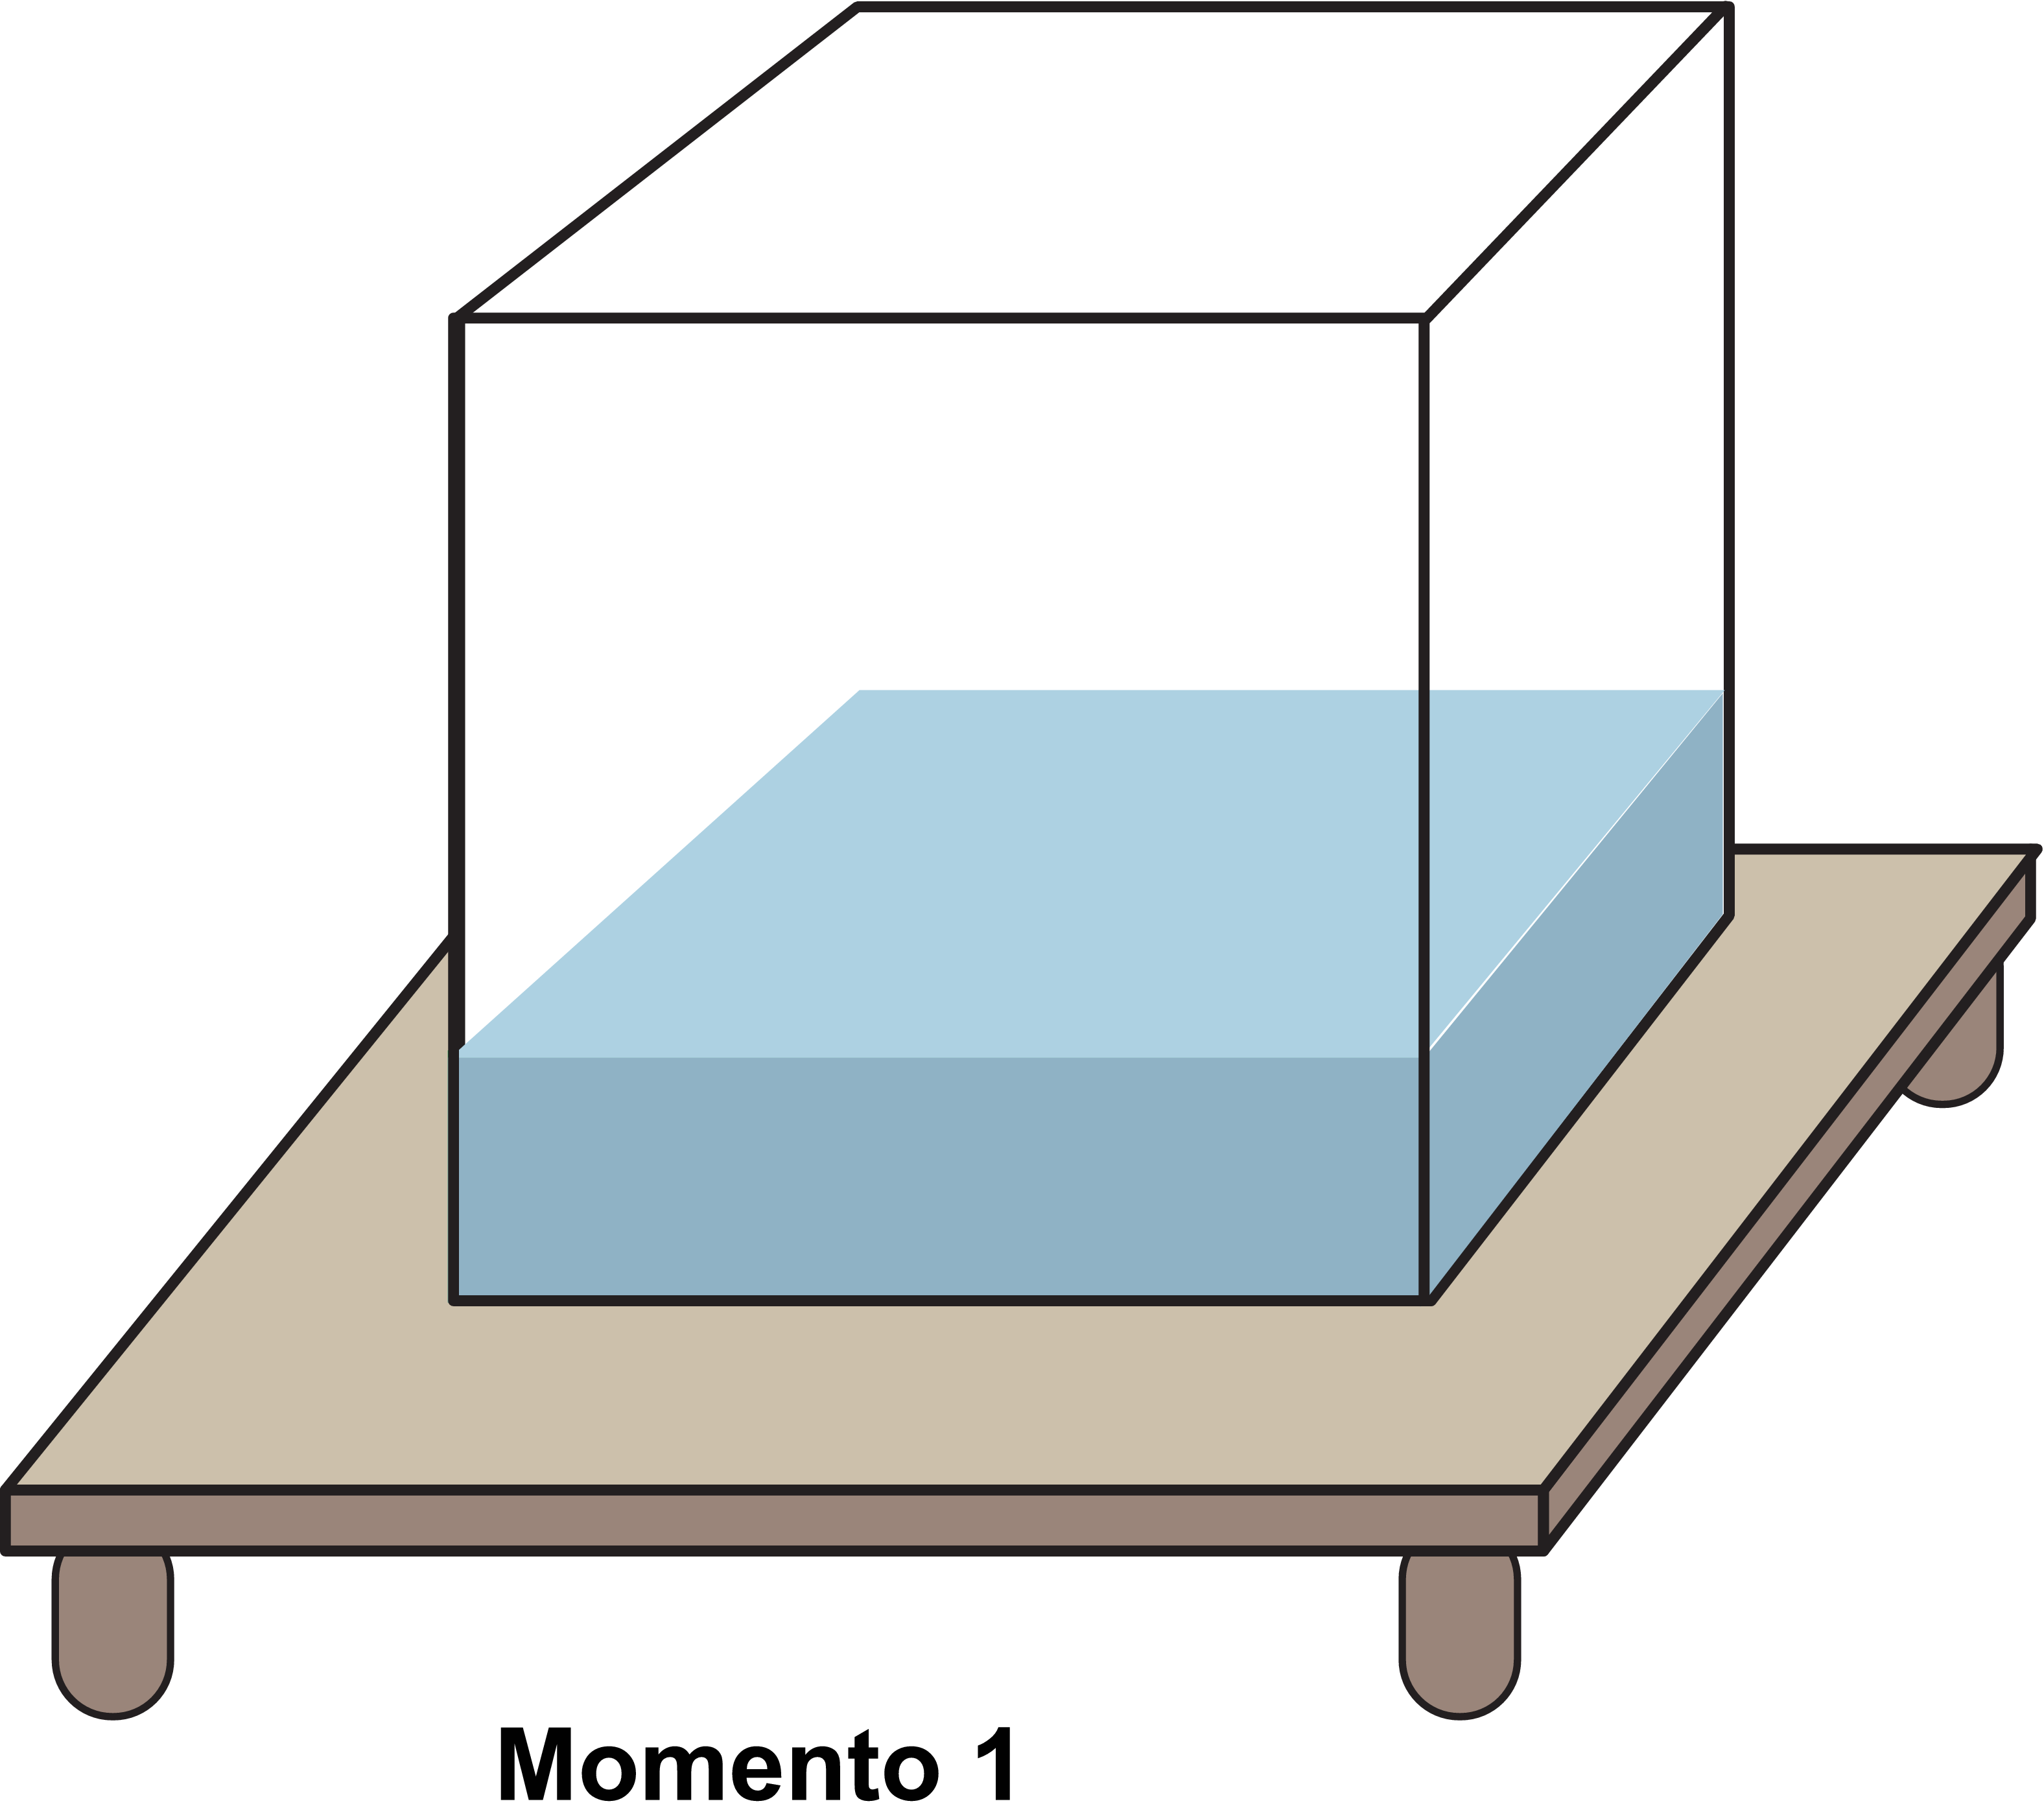
\includegraphics[width=145pt, keepaspectratio]{..//media/cap3/secoes/png/ativ1_fig01.png}  & 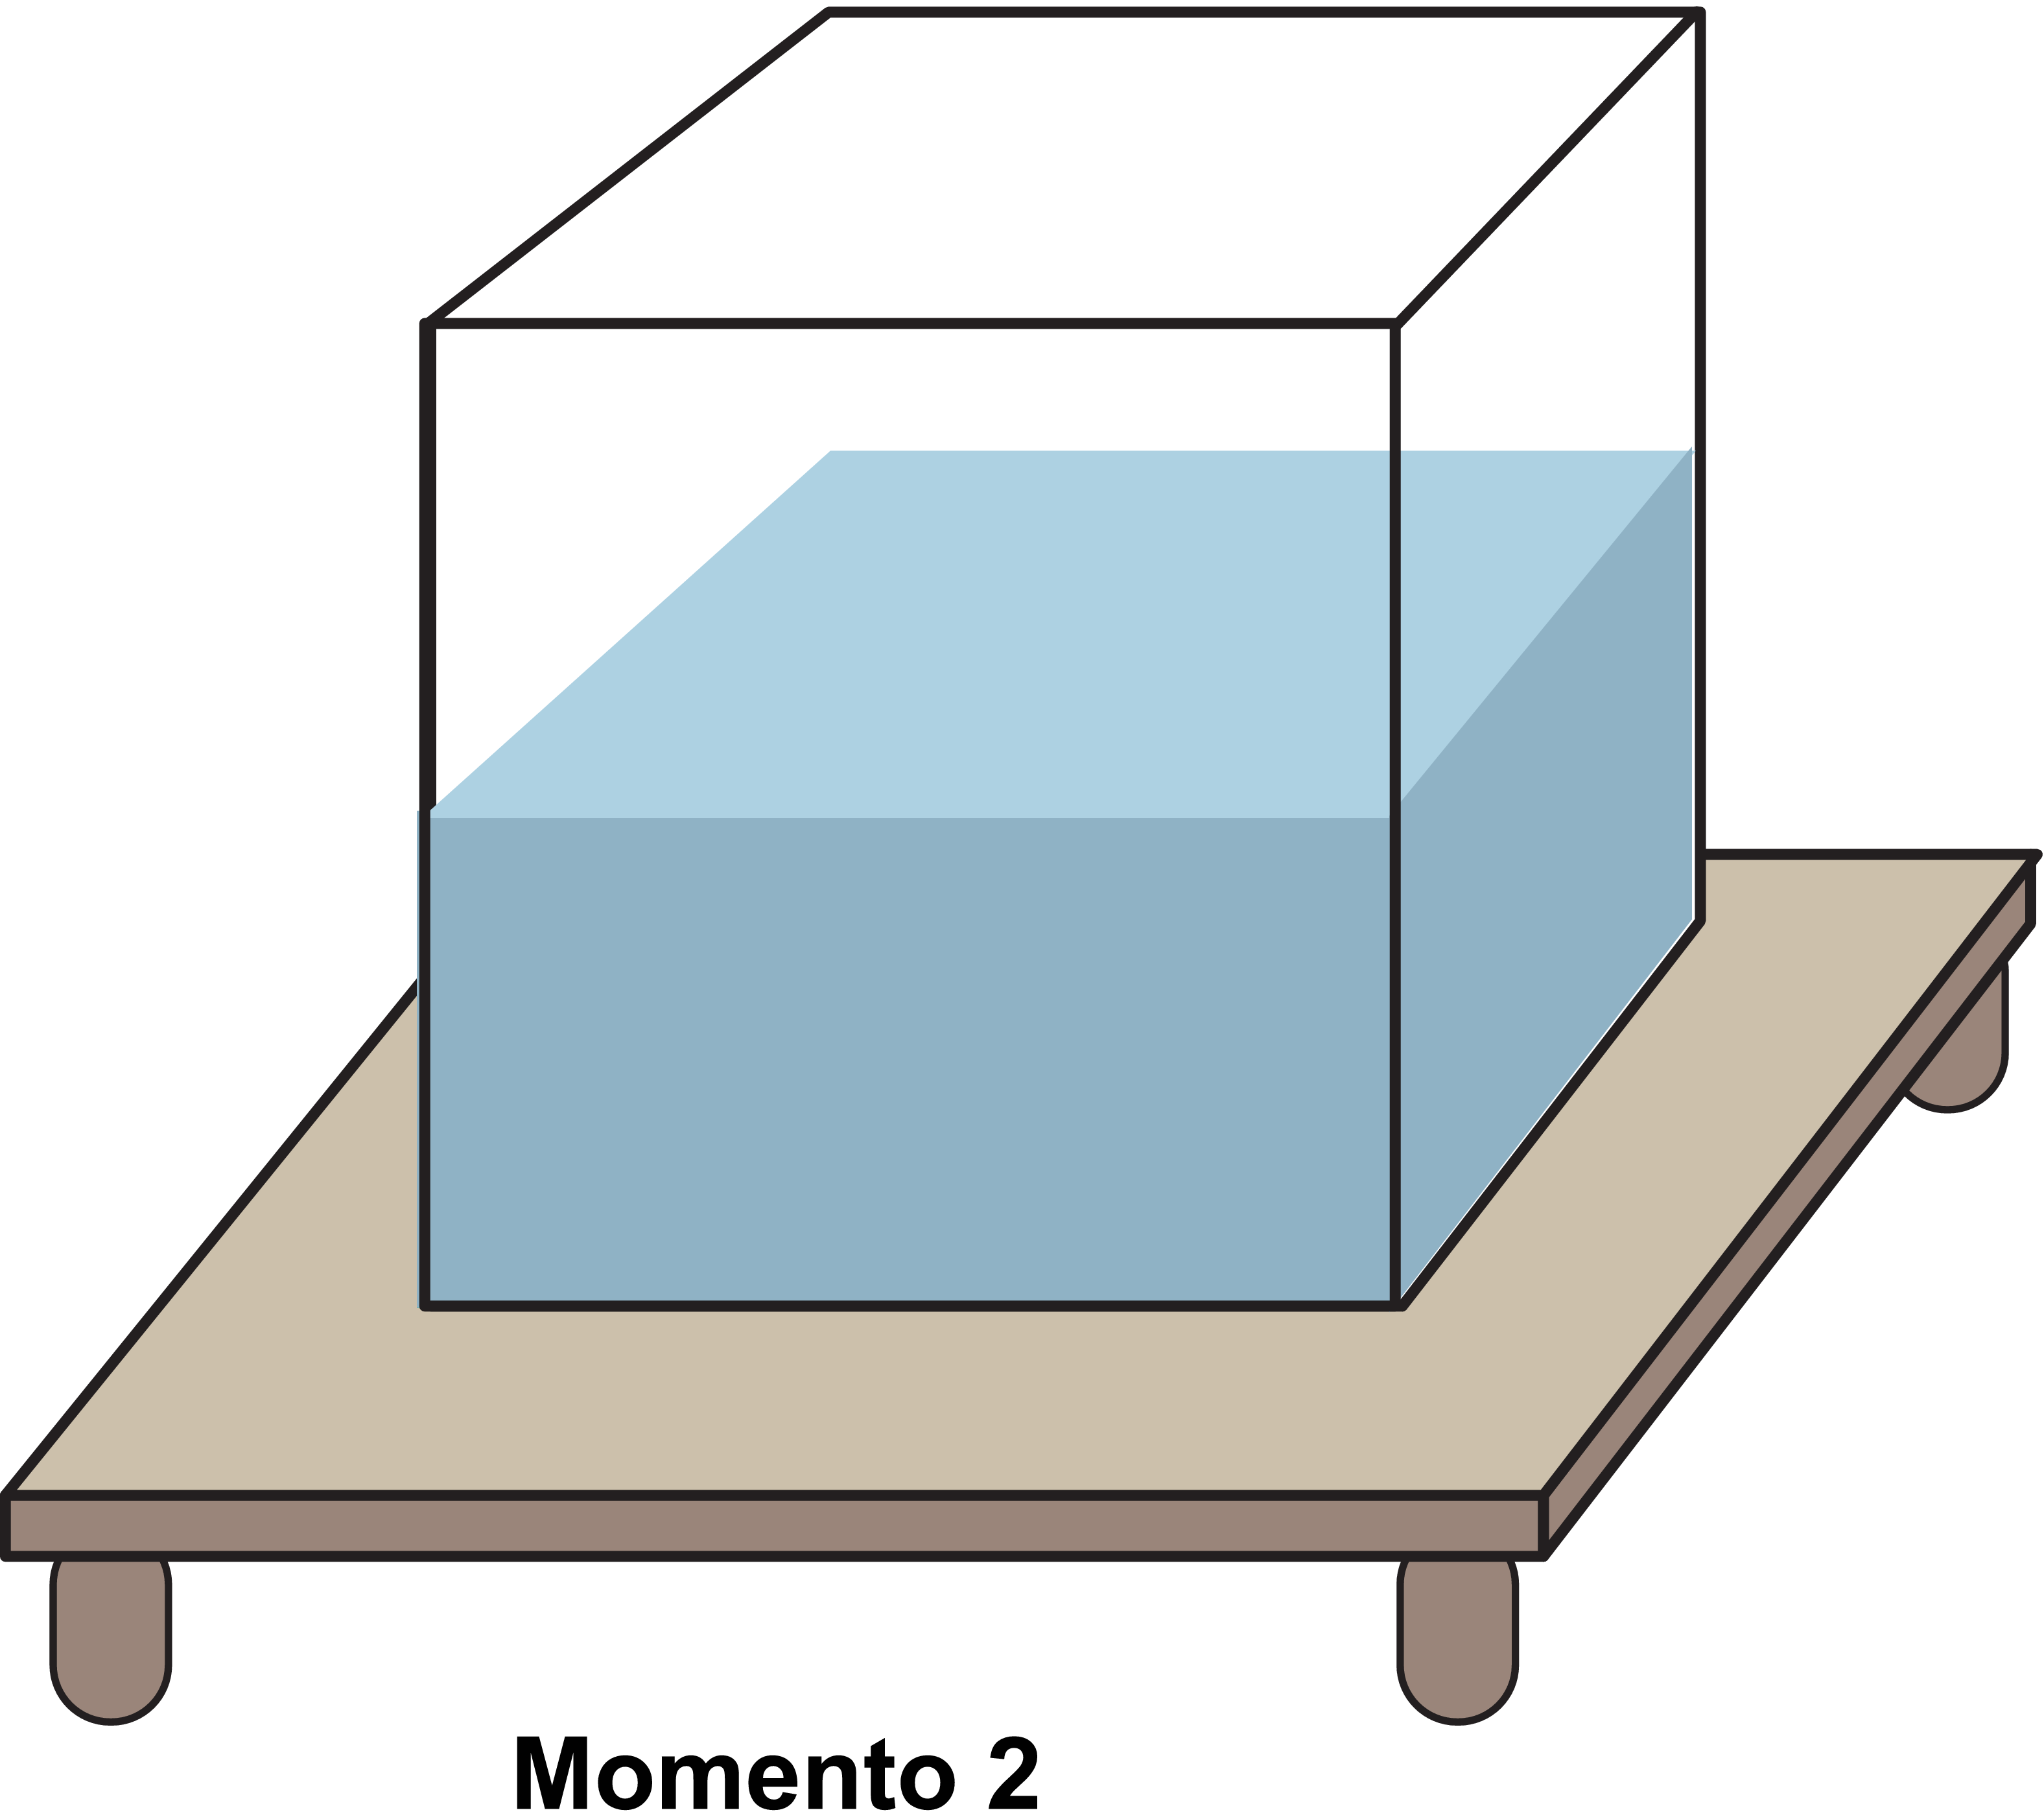
\includegraphics[width=145pt, keepaspectratio]{..//media/cap3/secoes/png/ativ1_fig02.png}
  \end{tabular}\newline
  \begin{tabular}{cc}
  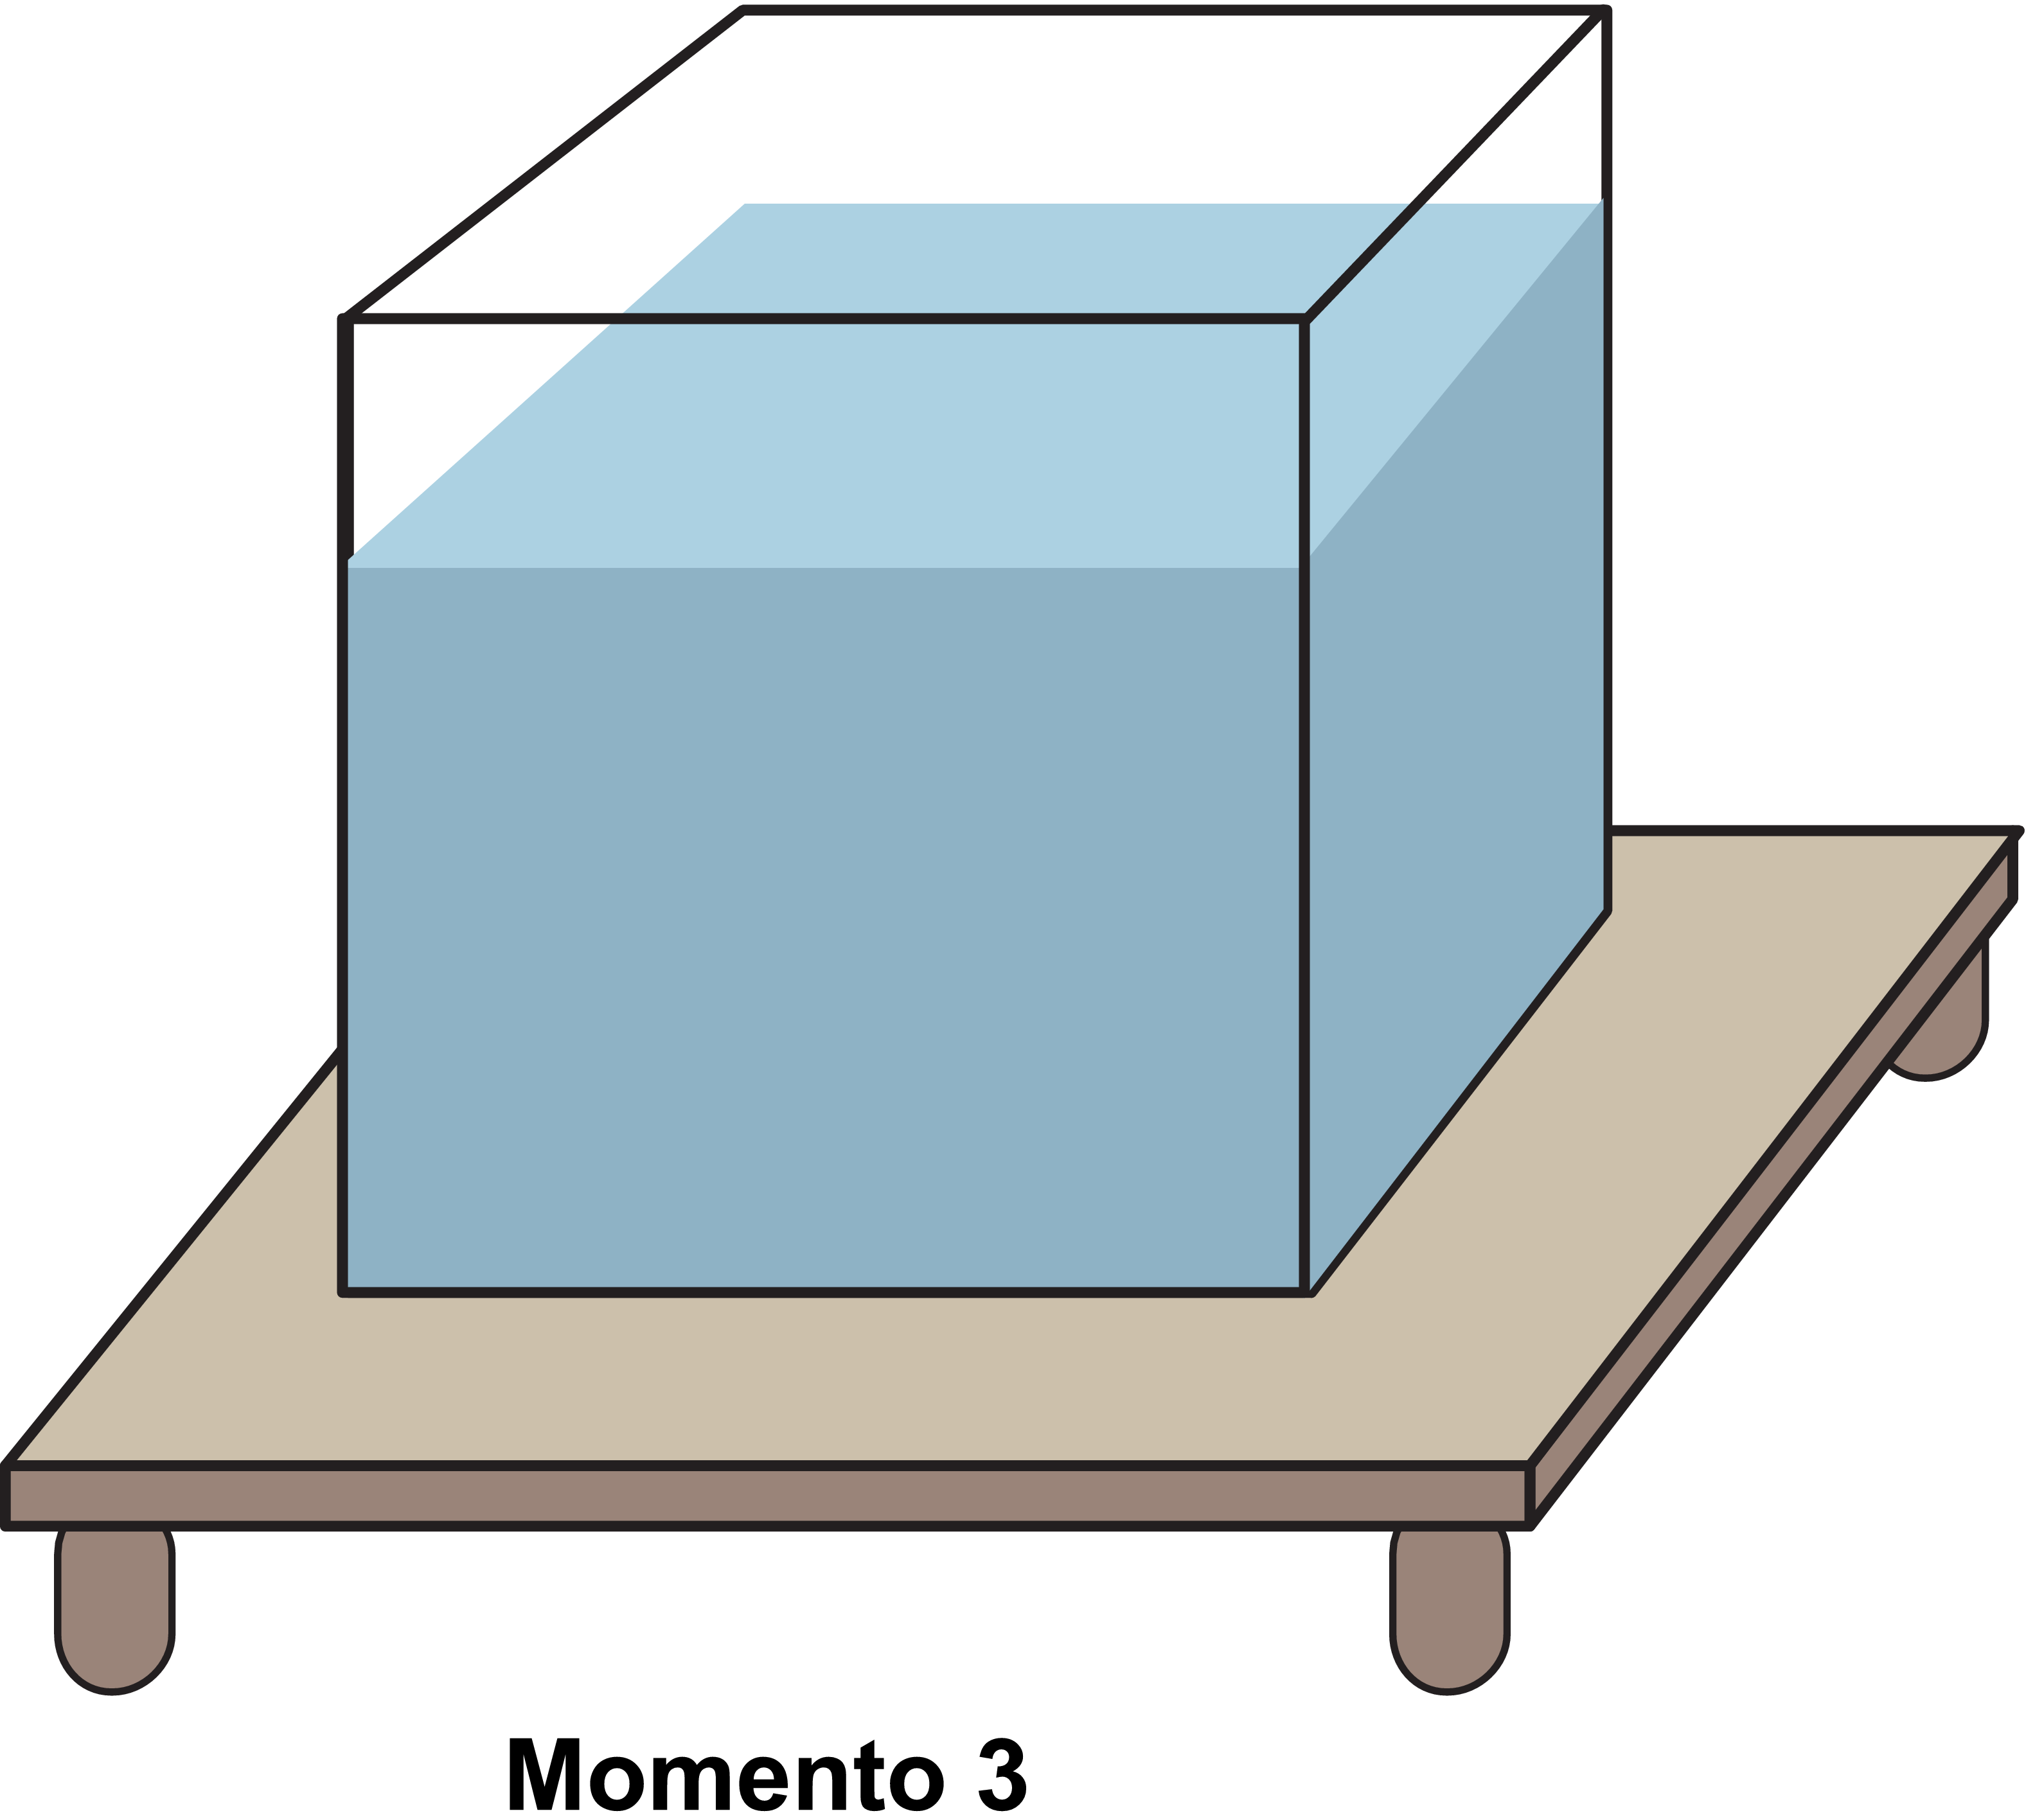
\includegraphics[width=145pt, keepaspectratio]{..//media/cap3/secoes/png/ativ1_fig03.png}  & 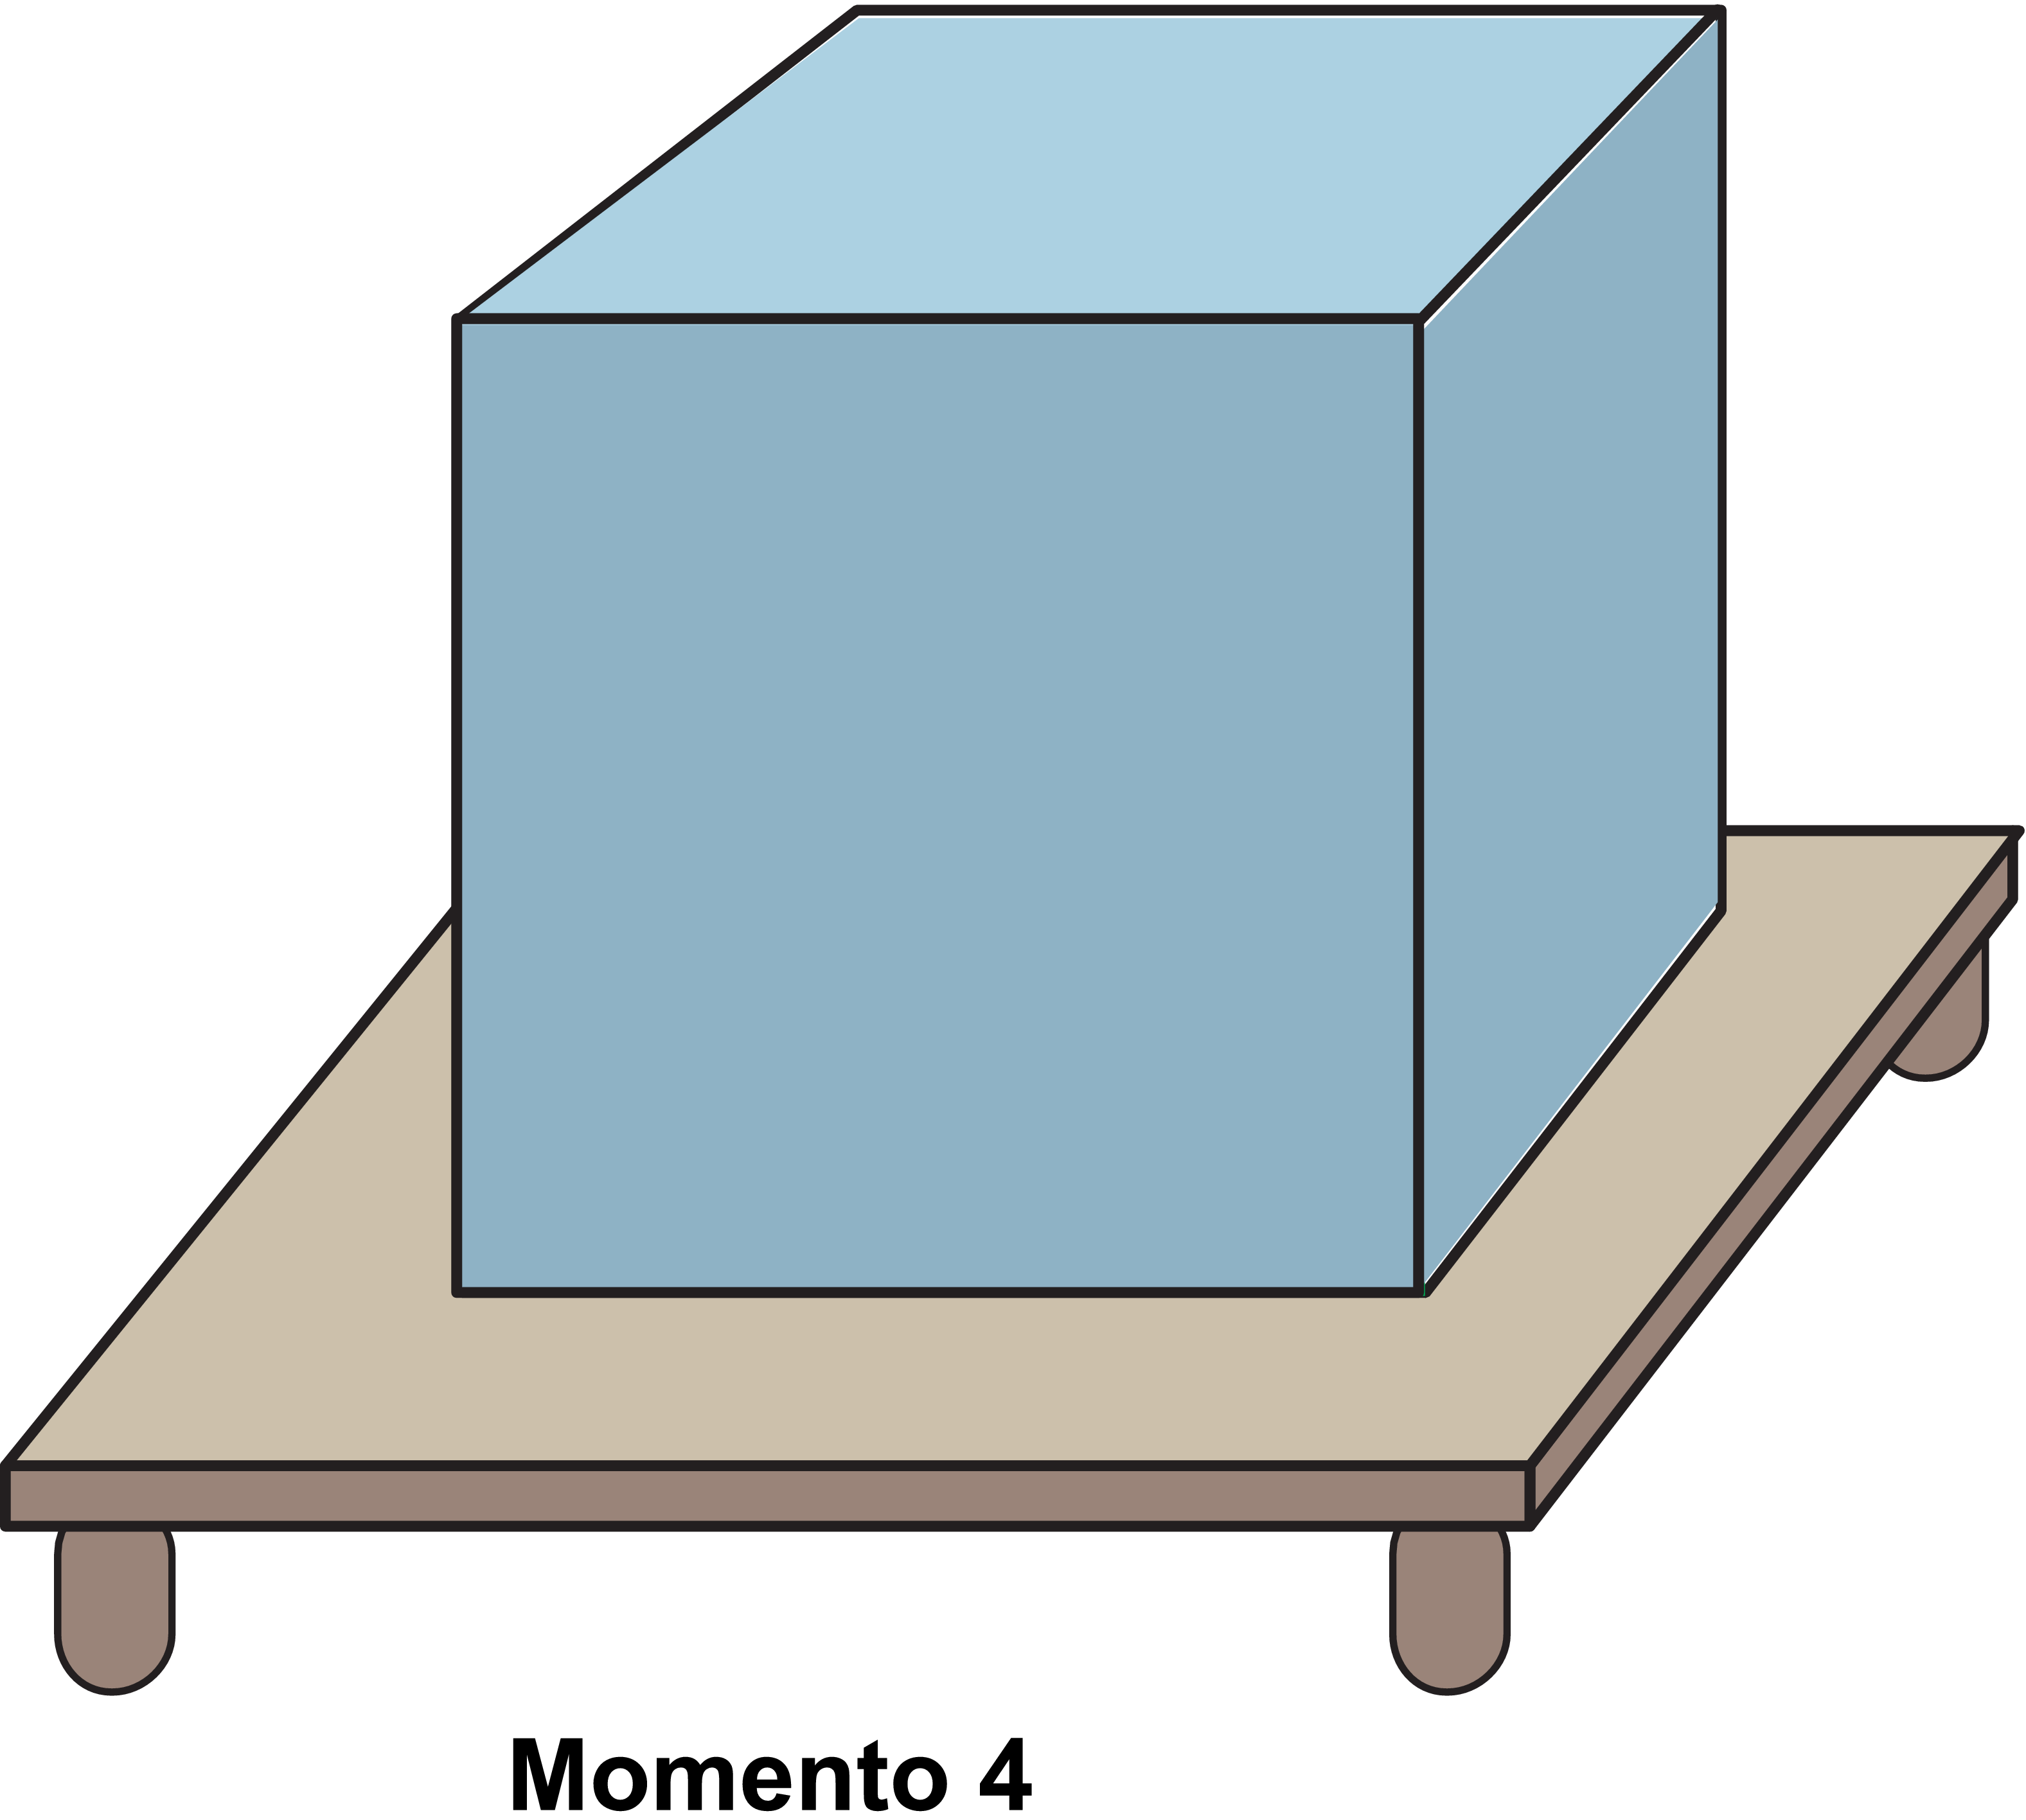
\includegraphics[width=145pt, keepaspectratio]{..//media/cap3/secoes/png/ativ1_fig04.png}
  \end{tabular}
  \end{center}

Escolha, para cada um dos momentos, a graduação que lhe parece mais adequada para registrar a quantidade de agua representada em cada uma das imagens. Explique sua escolha.

  
     \begin{center}
     \begin{tabular}{m{.3\textwidth}m{.3\textwidth}m{.3\textwidth}}
 \parbox[b][.3cm][t]{.3cm}{a)}  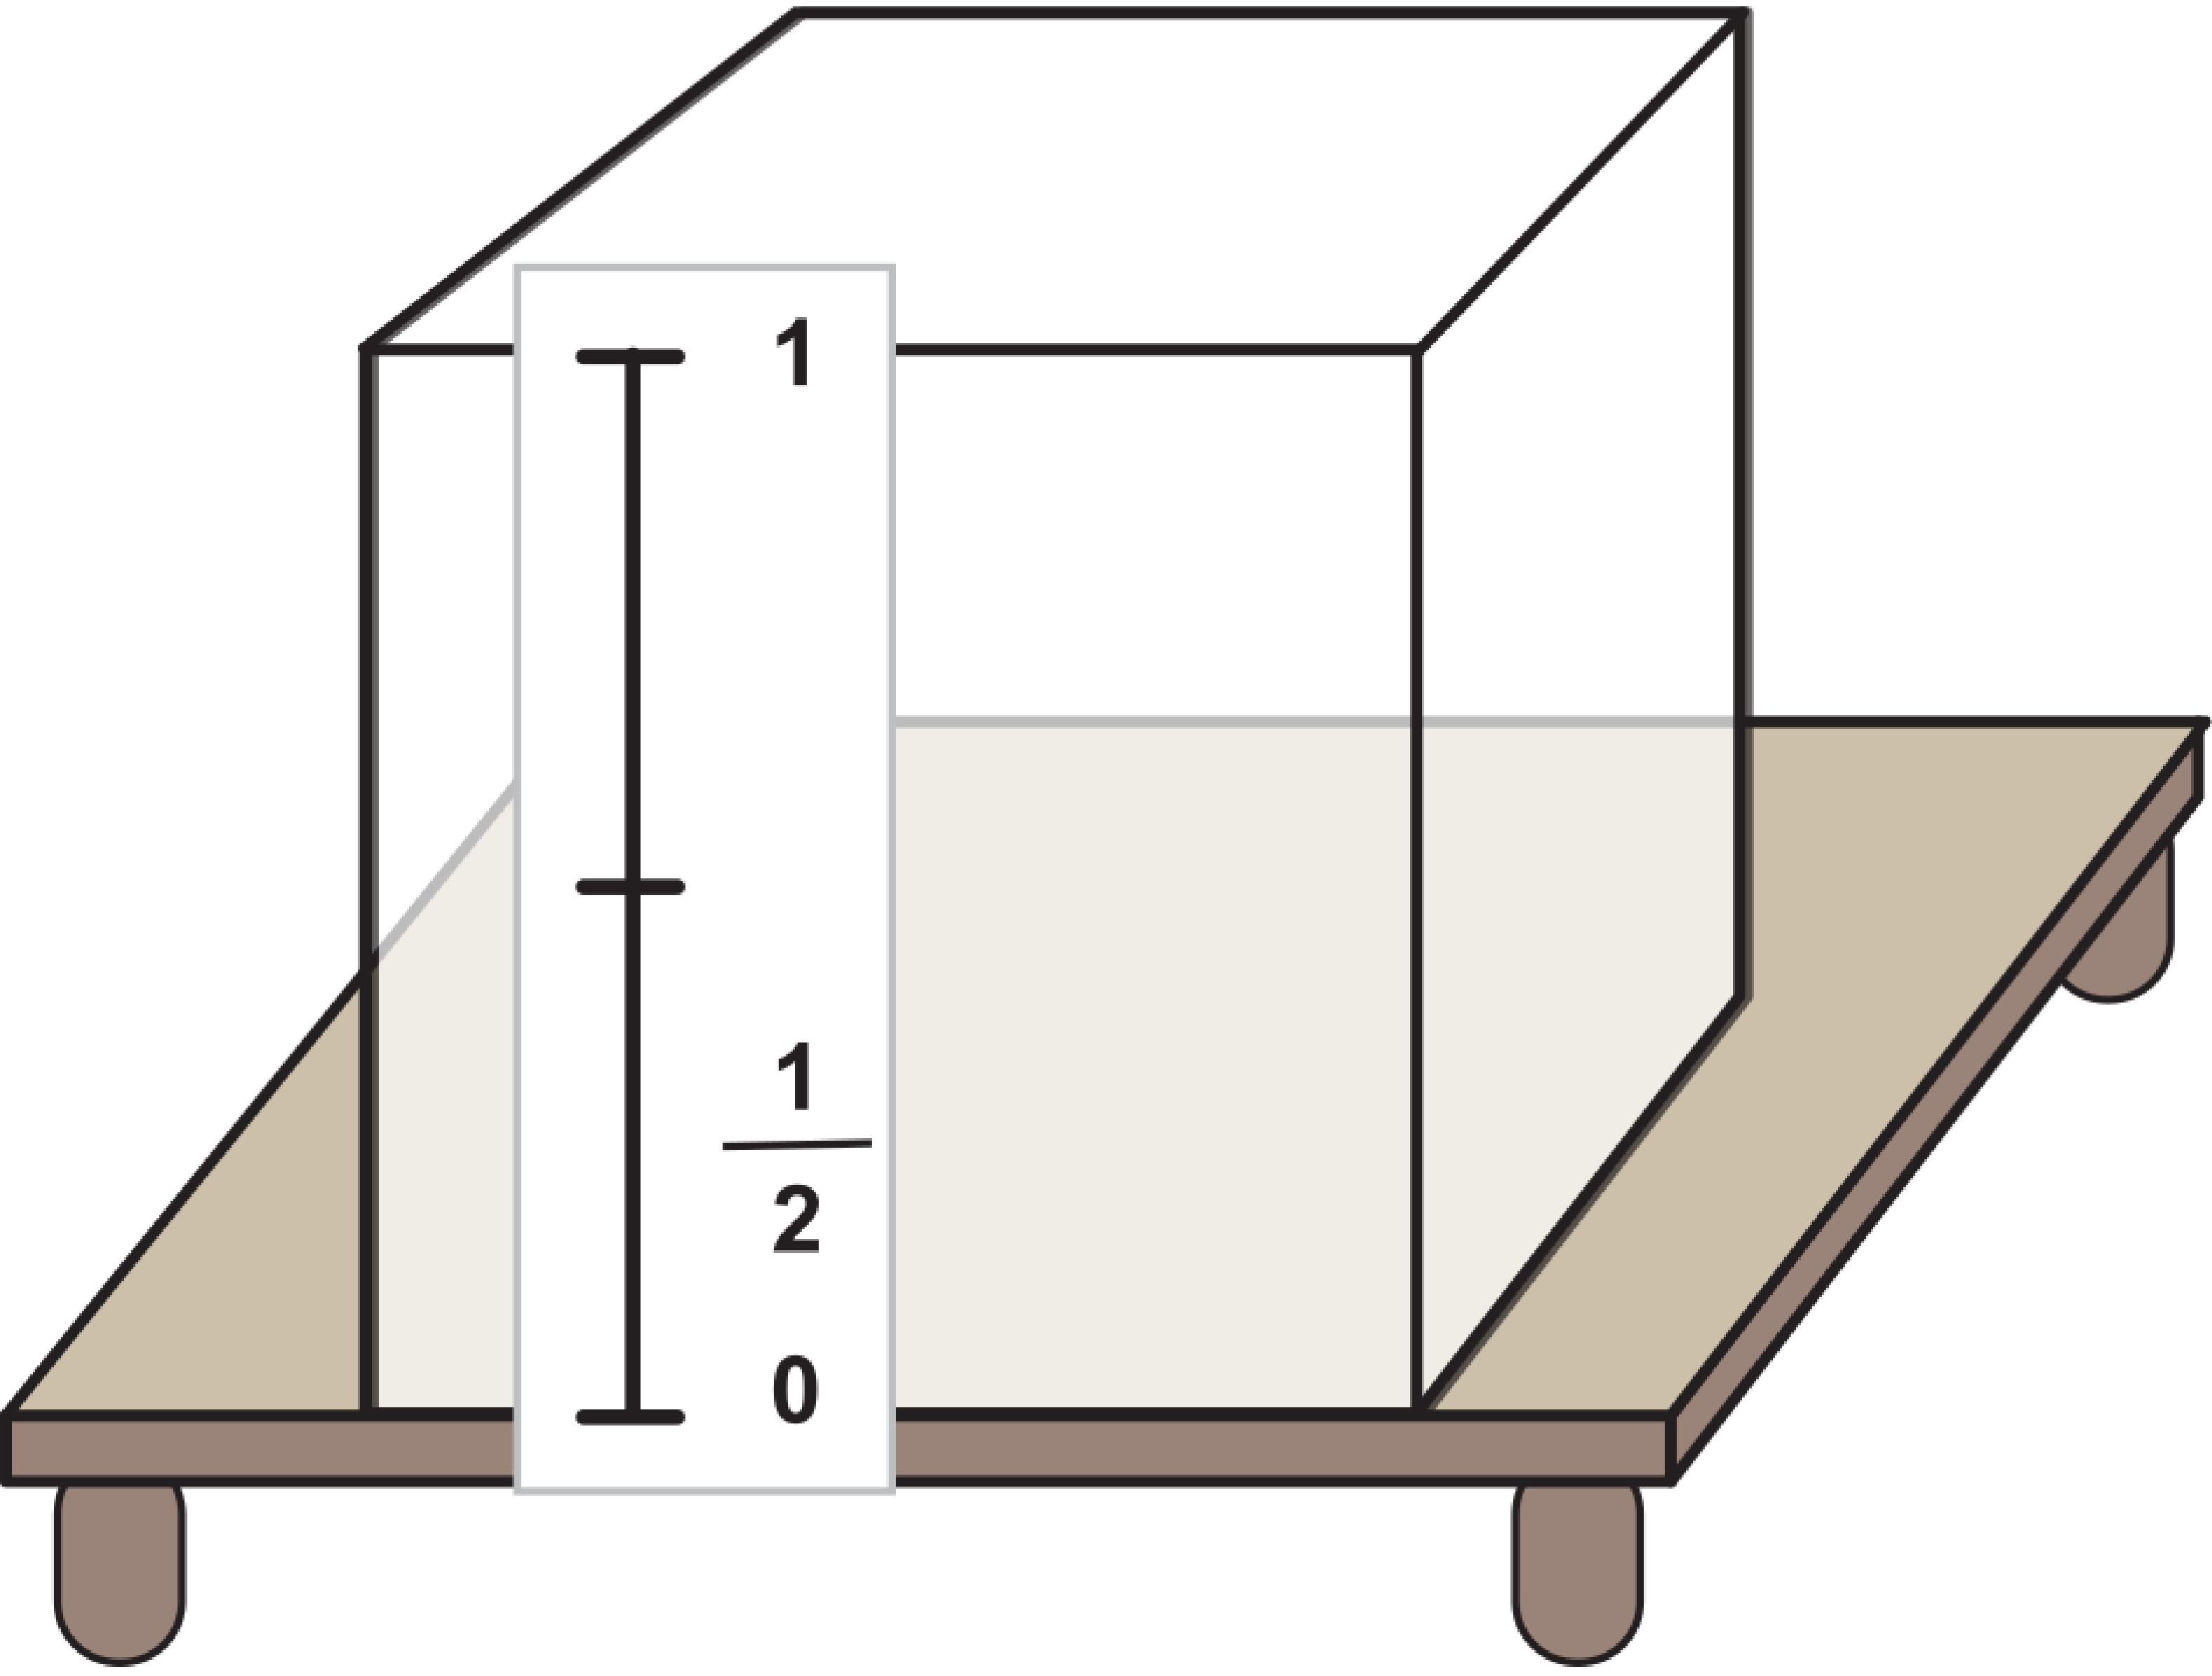
\includegraphics[width=145pt, keepaspectratio]{..//media/cap3/secoes/png/ativ1_fig05.png} &  
 \parbox[b][.3cm][t]{.3cm}{b)}  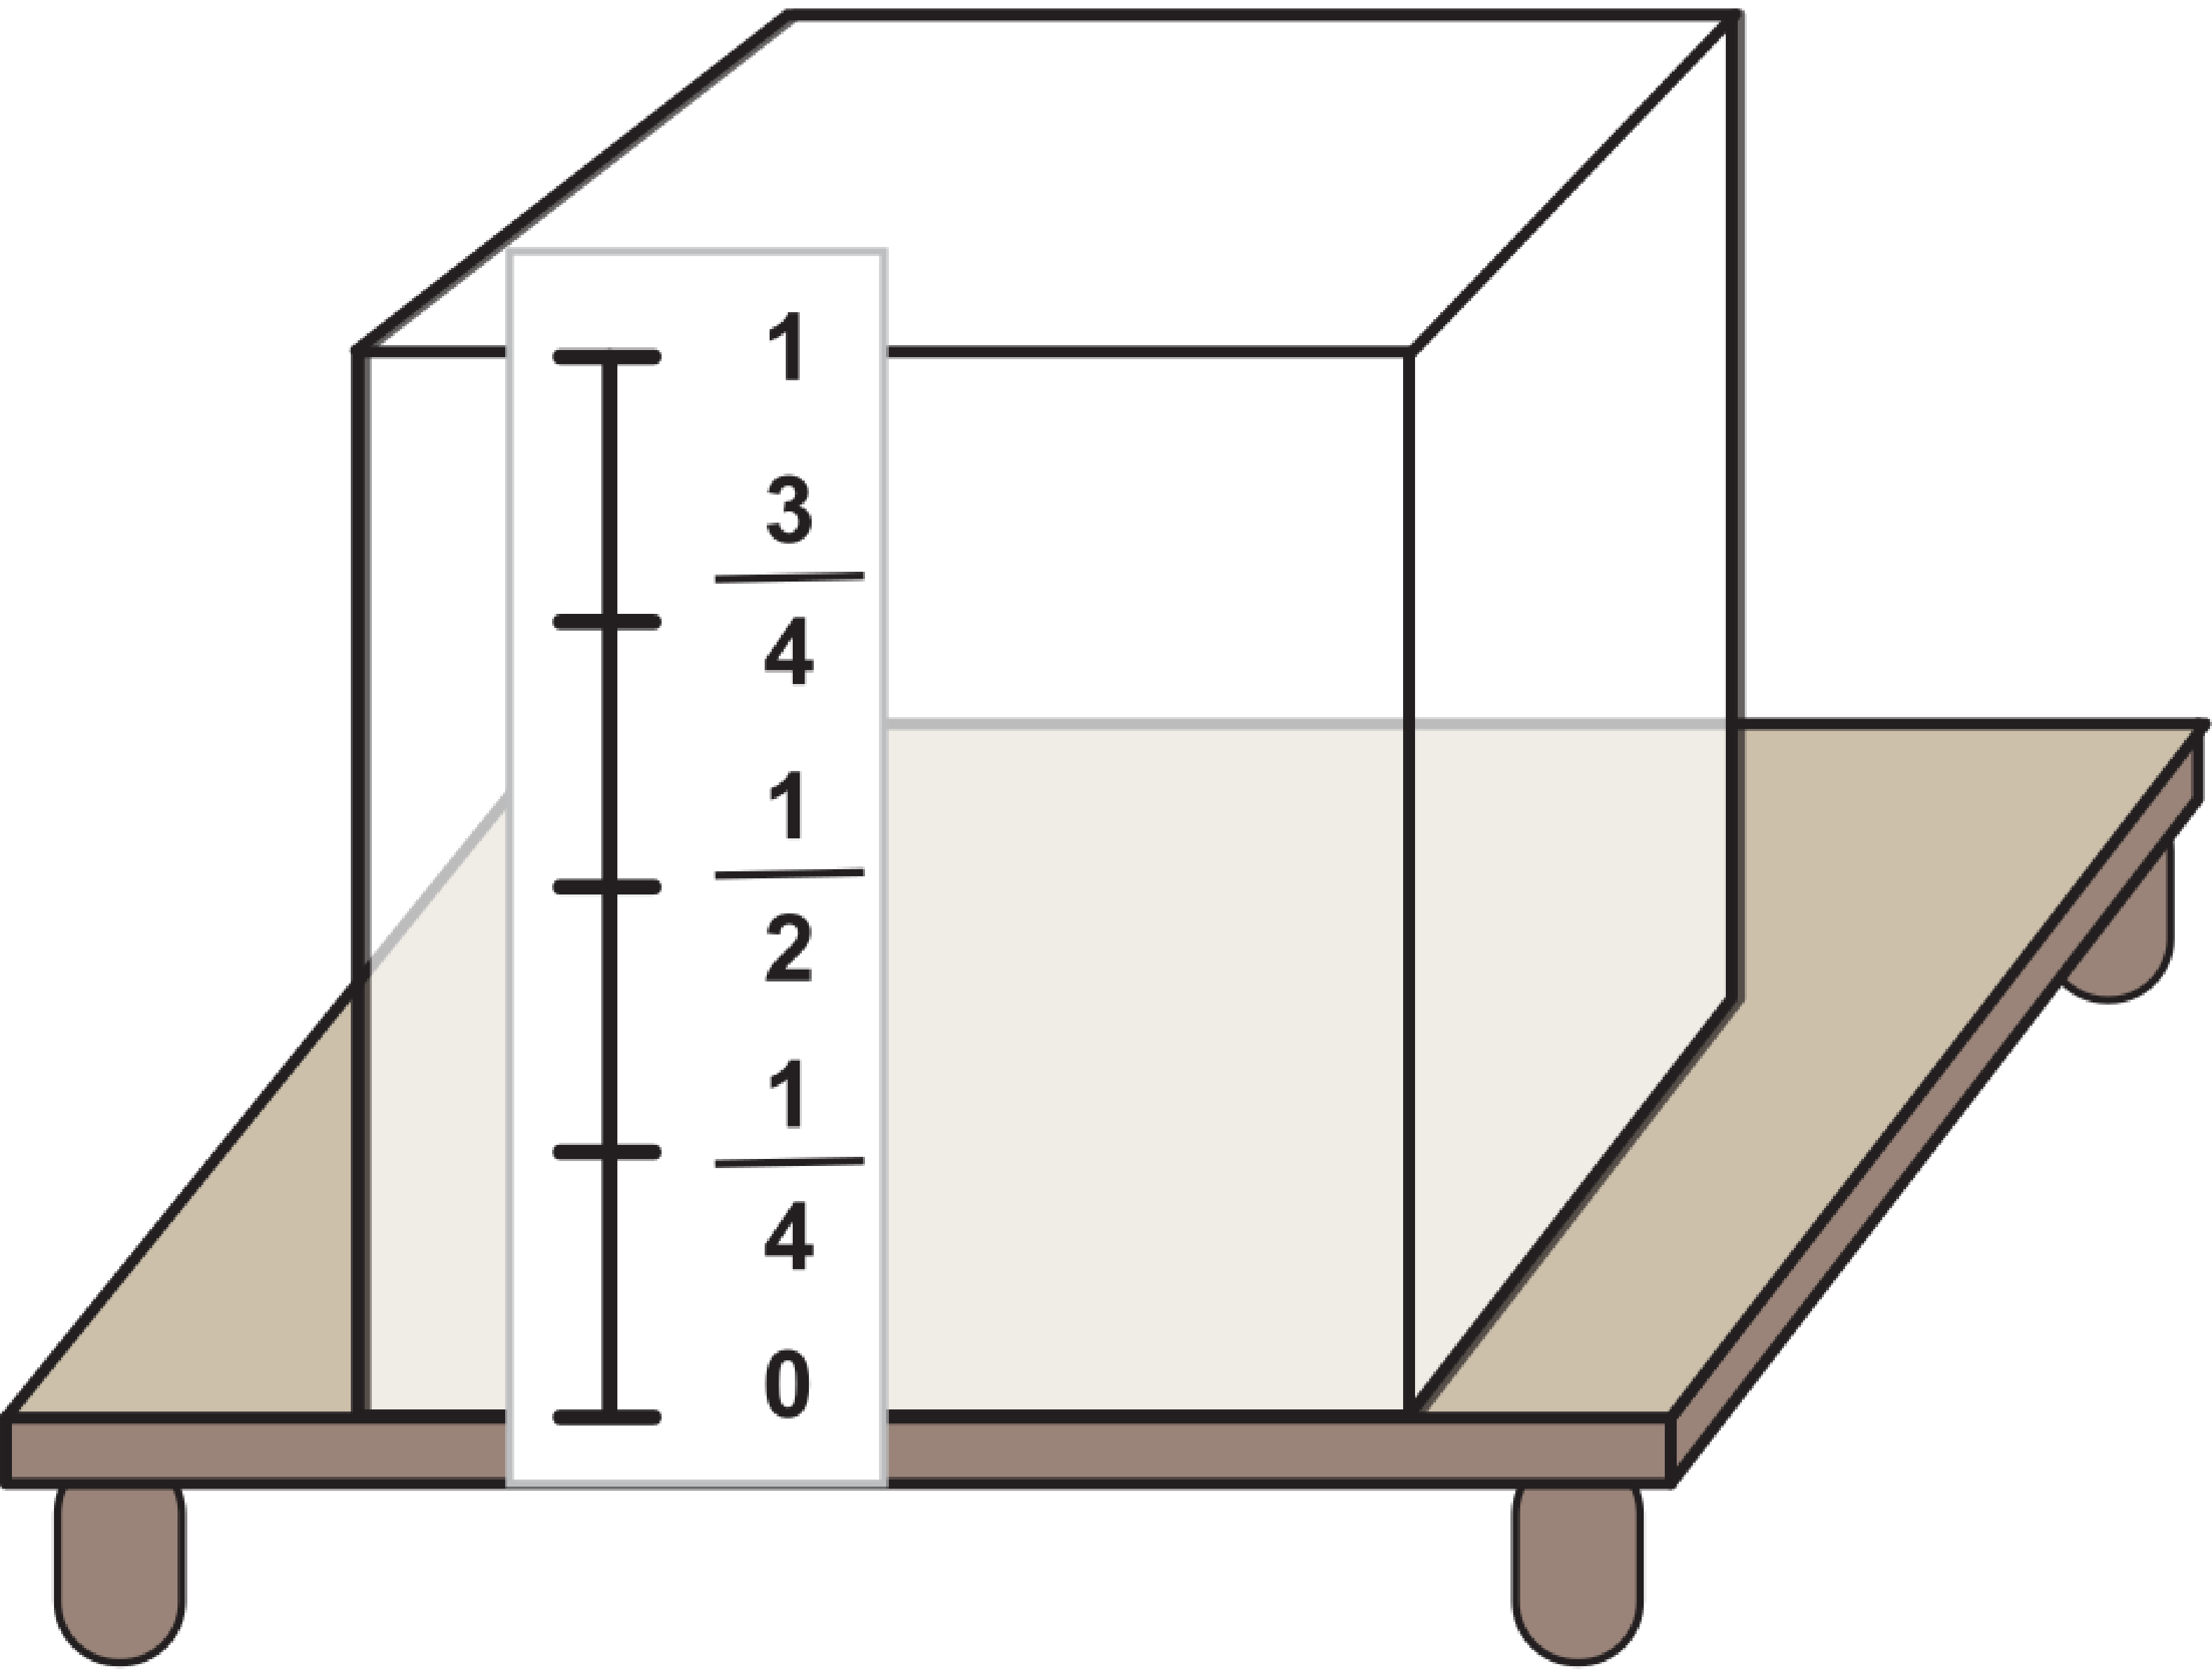
\includegraphics[width=145pt, keepaspectratio]{..//media/cap3/secoes/png/ativ1_fig06.png} &
  \parbox[b][.3cm][t]{.3cm}{c)}  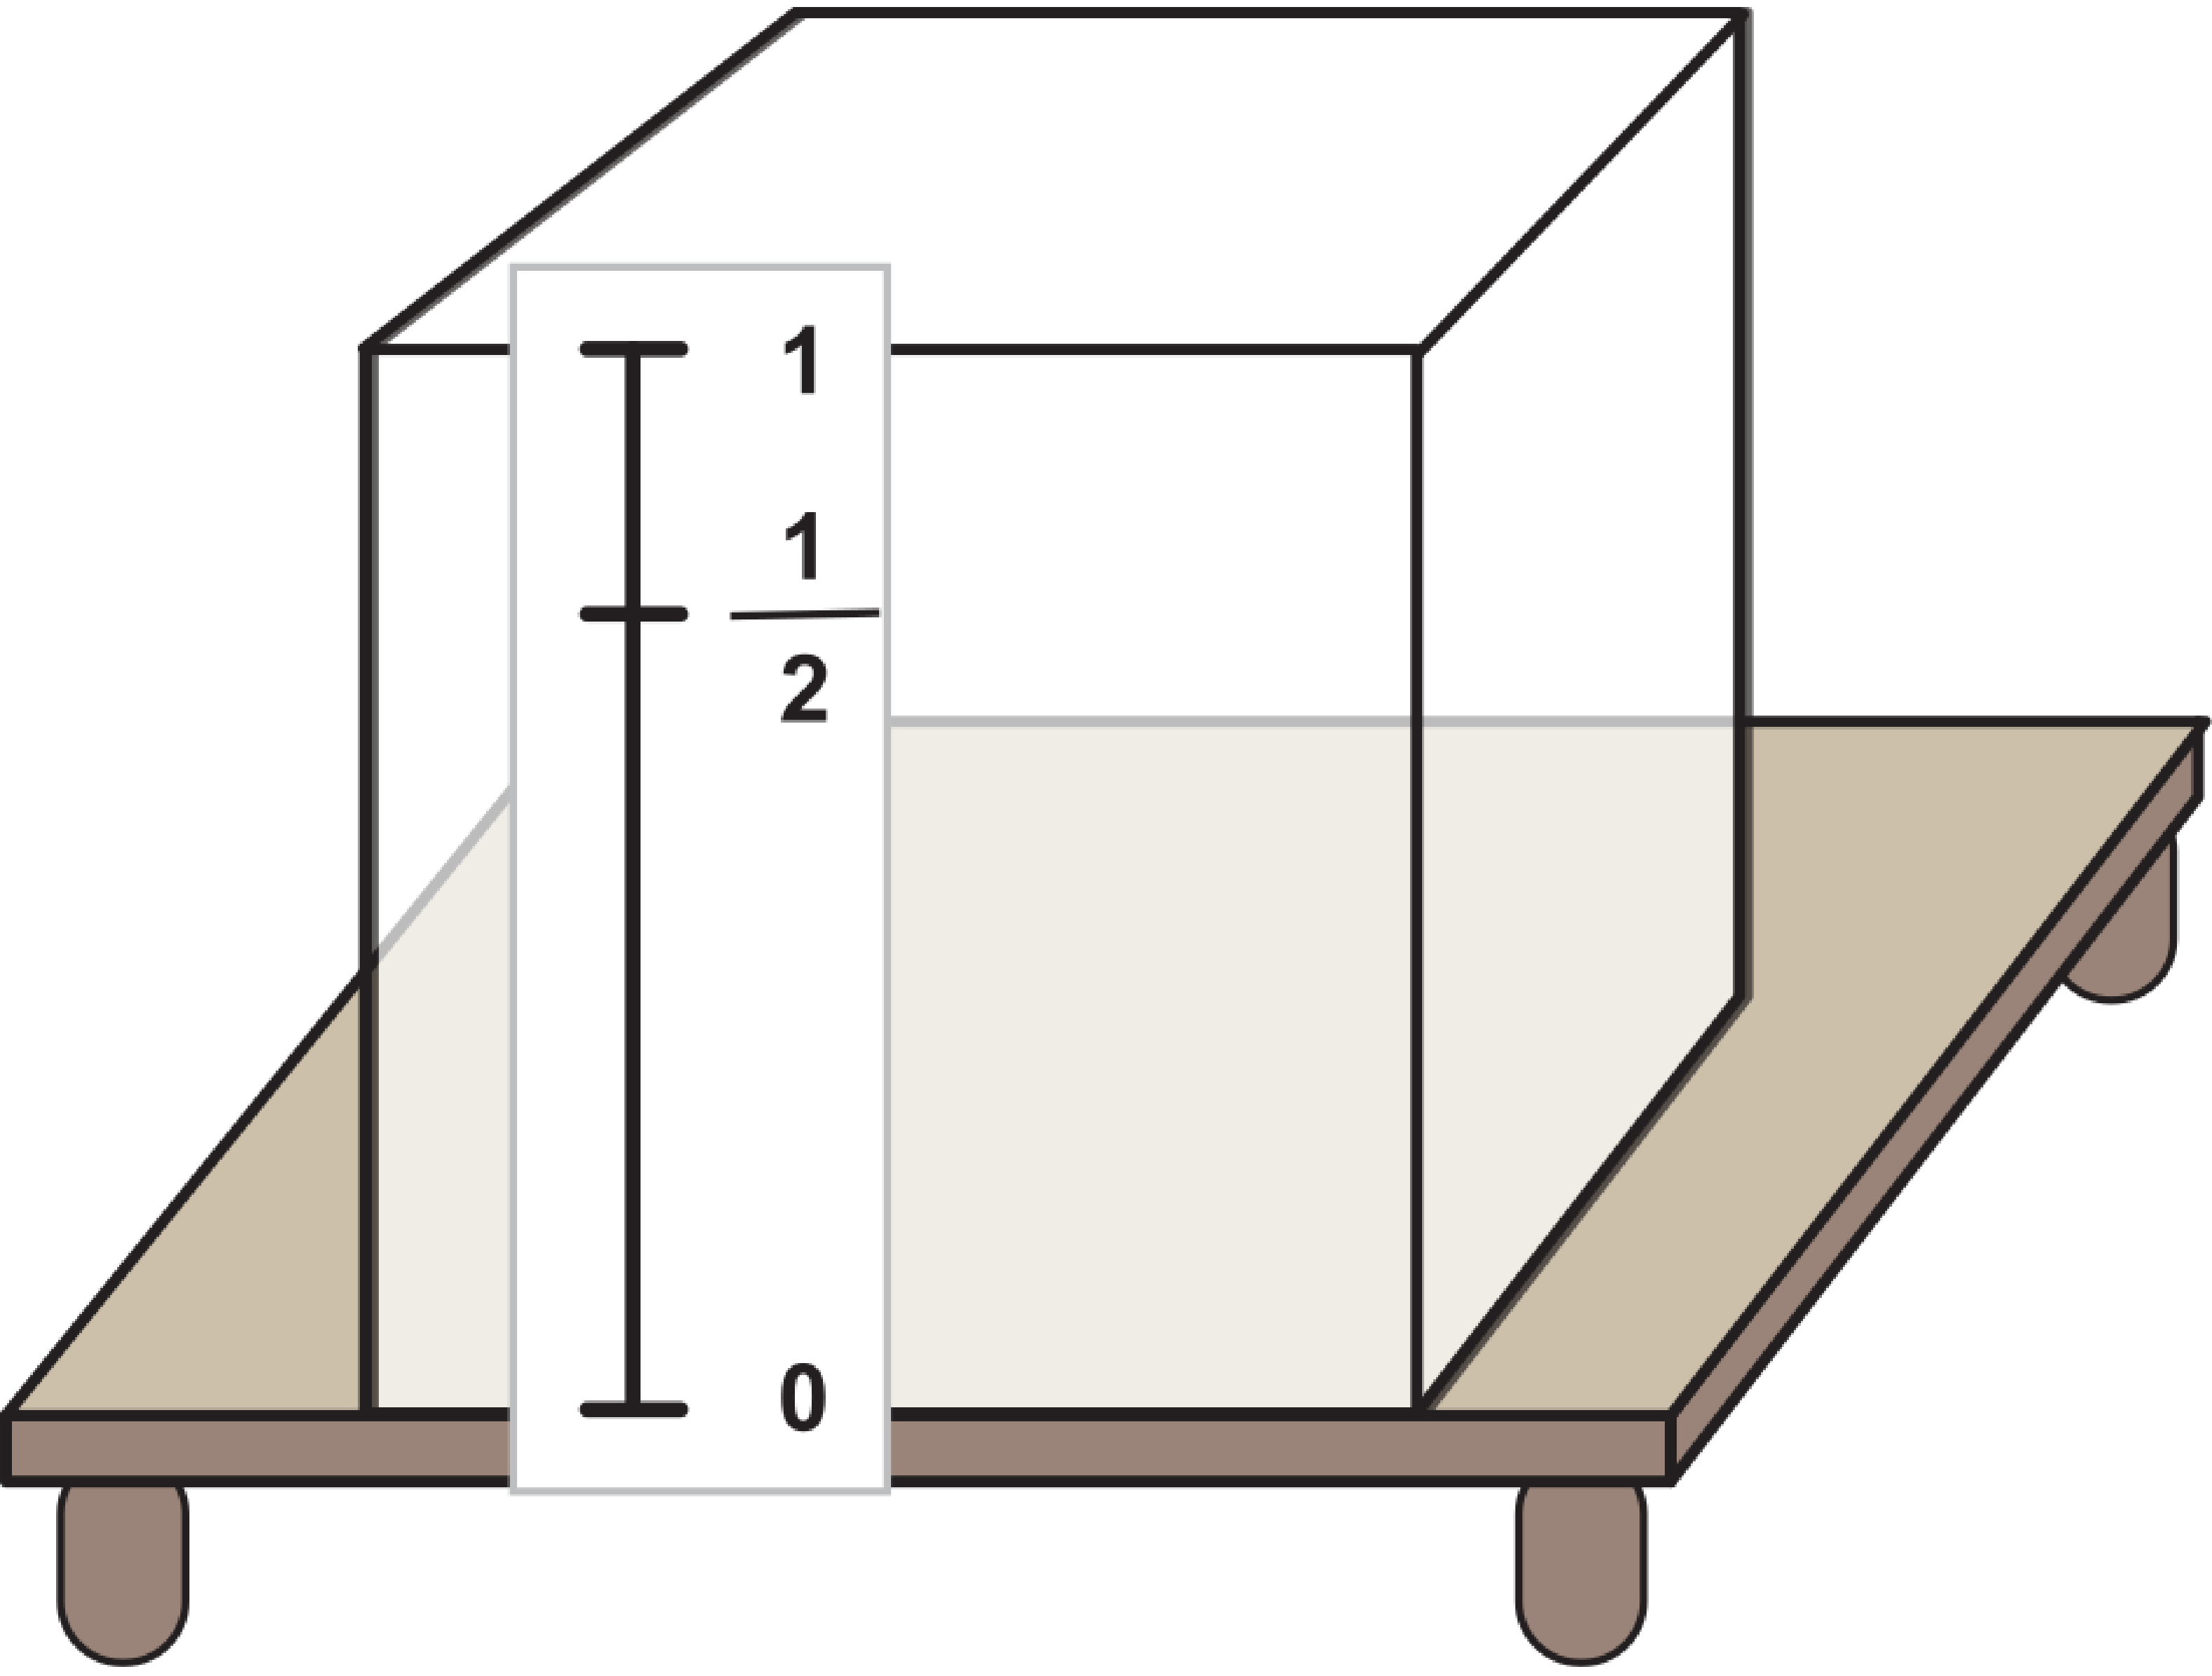
\includegraphics[width=145pt, keepaspectratio]{..//media/cap3/secoes/png/ativ1_fig07.png}  
   \end{tabular}
   
  \begin{tabular}{m{.3\textwidth}m{.3\textwidth}}
  \parbox[b][0.3cm][t]{.3cm}{d)}  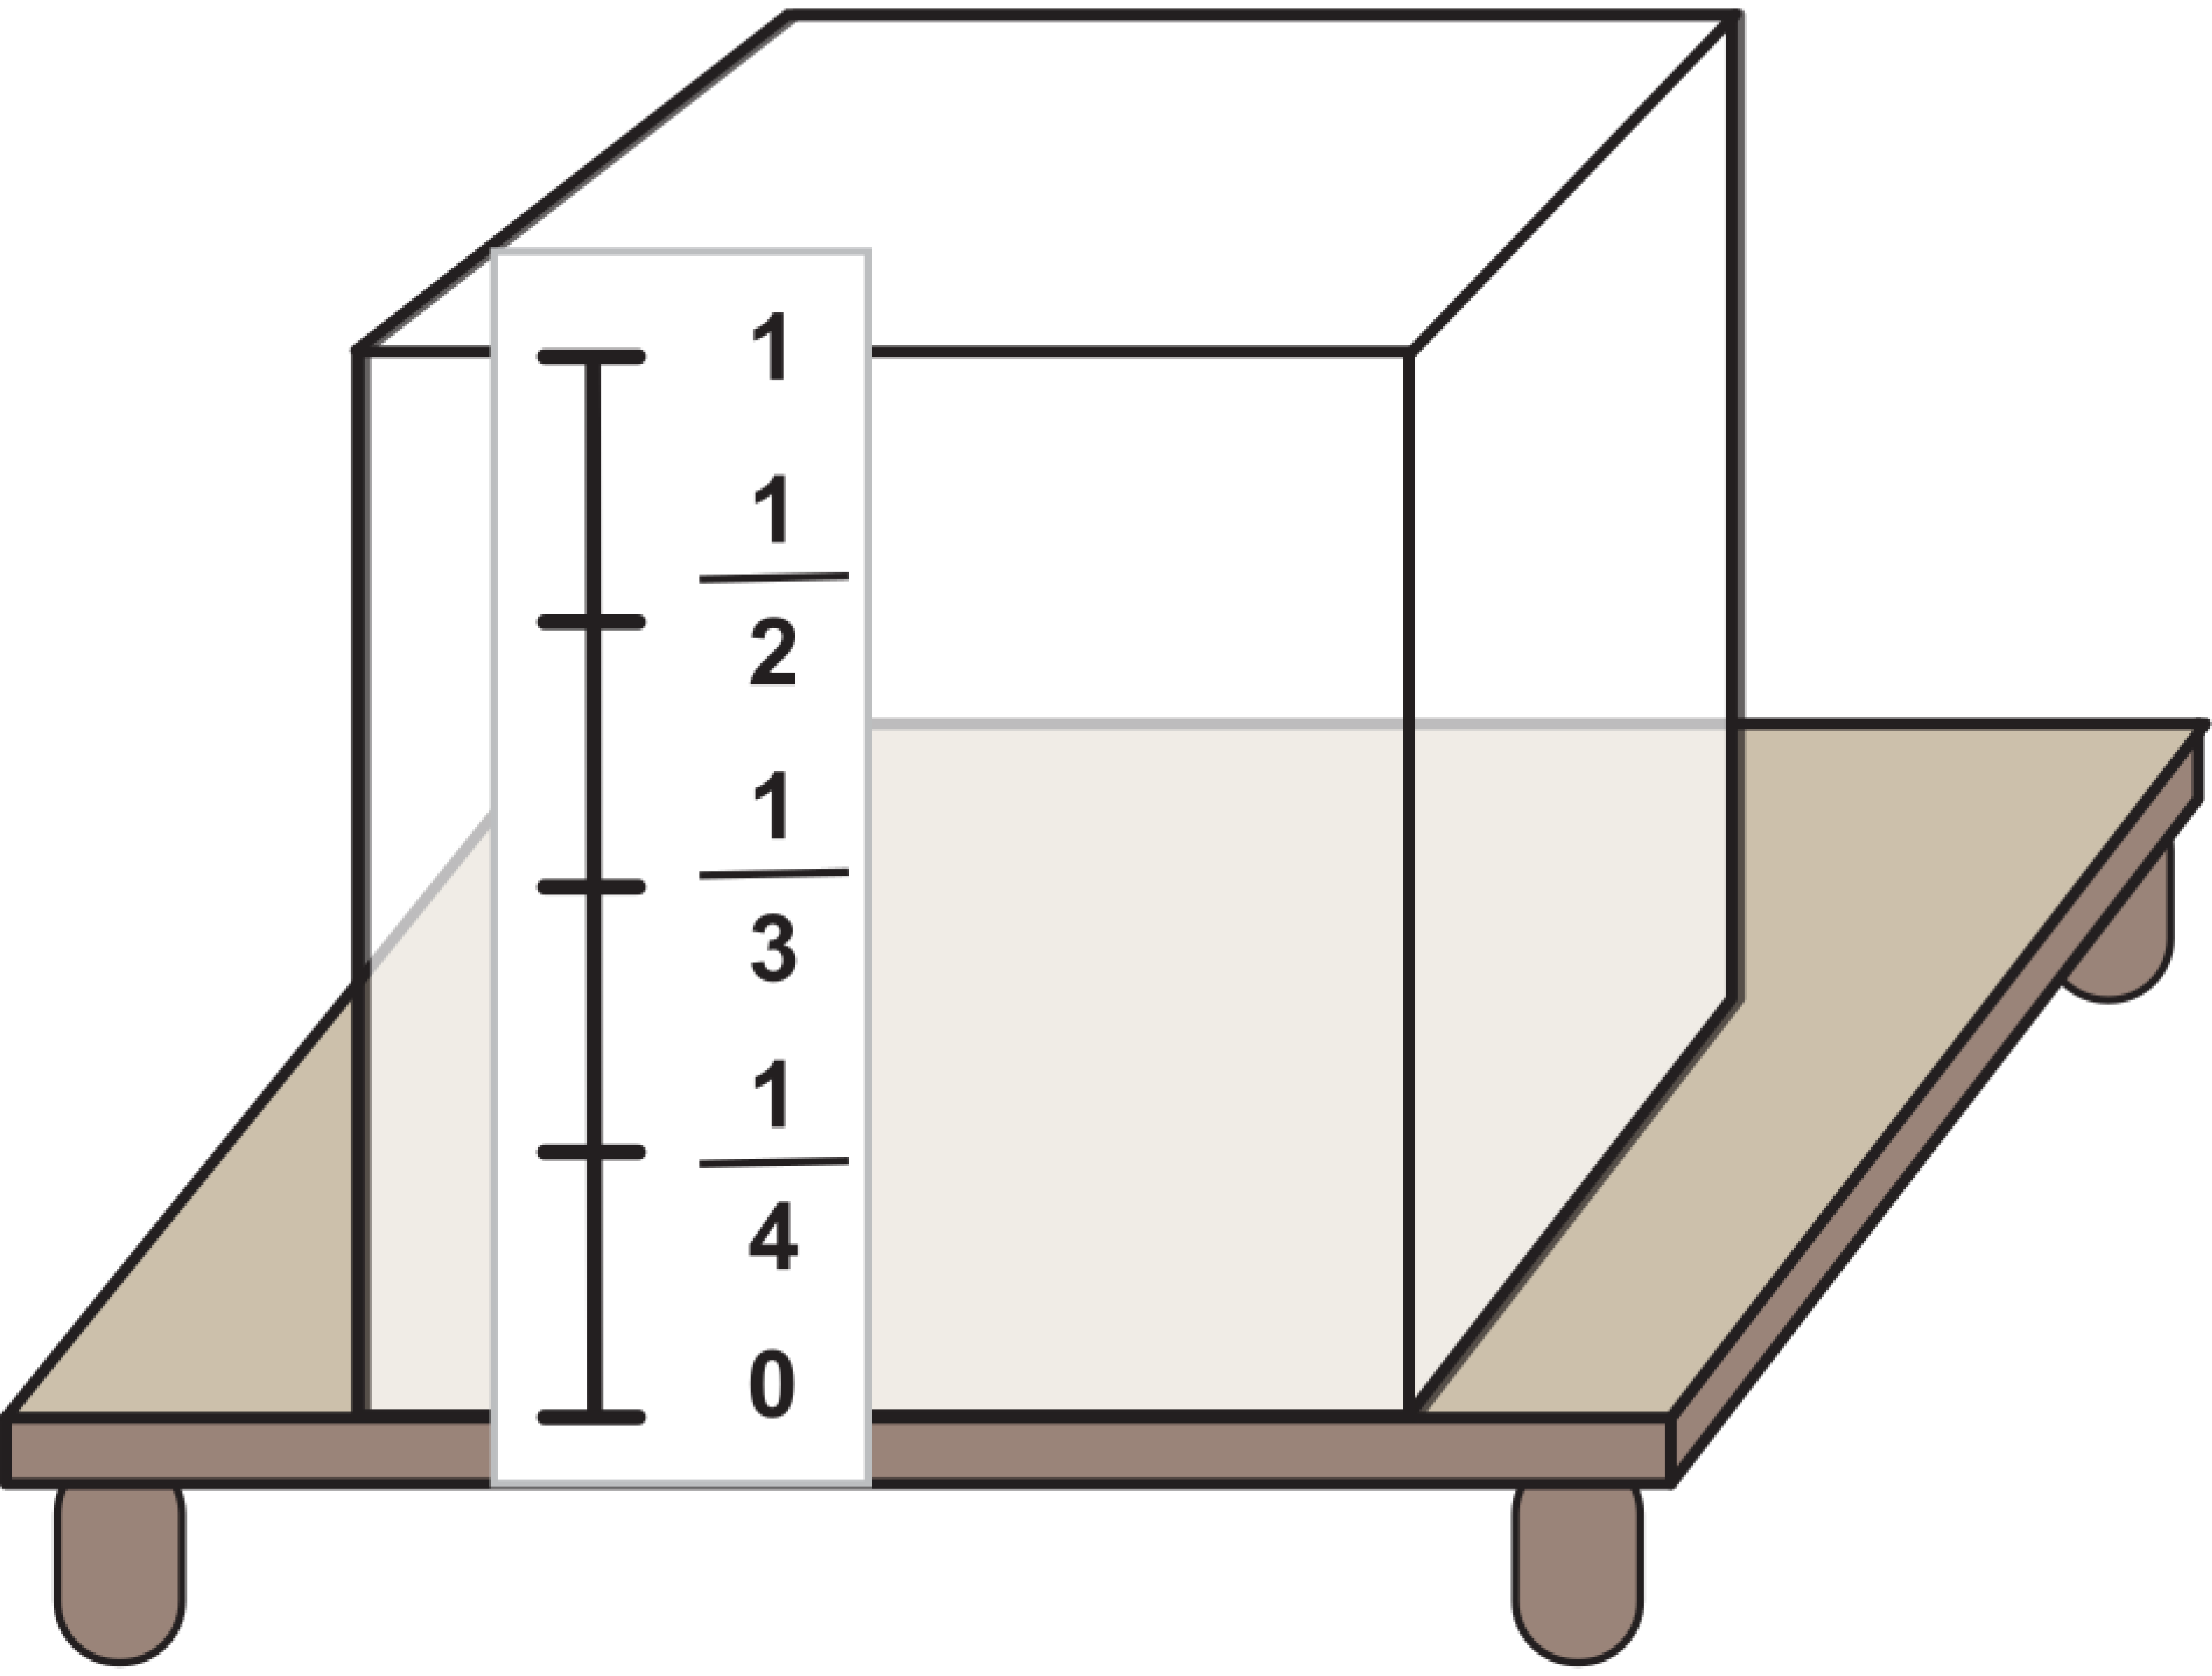
\includegraphics[width=145pt, keepaspectratio]{..//media/cap3/secoes/png/ativ1_fig08.png}&
  \parbox[b][0.3cm][t]{.3cm}{e)}  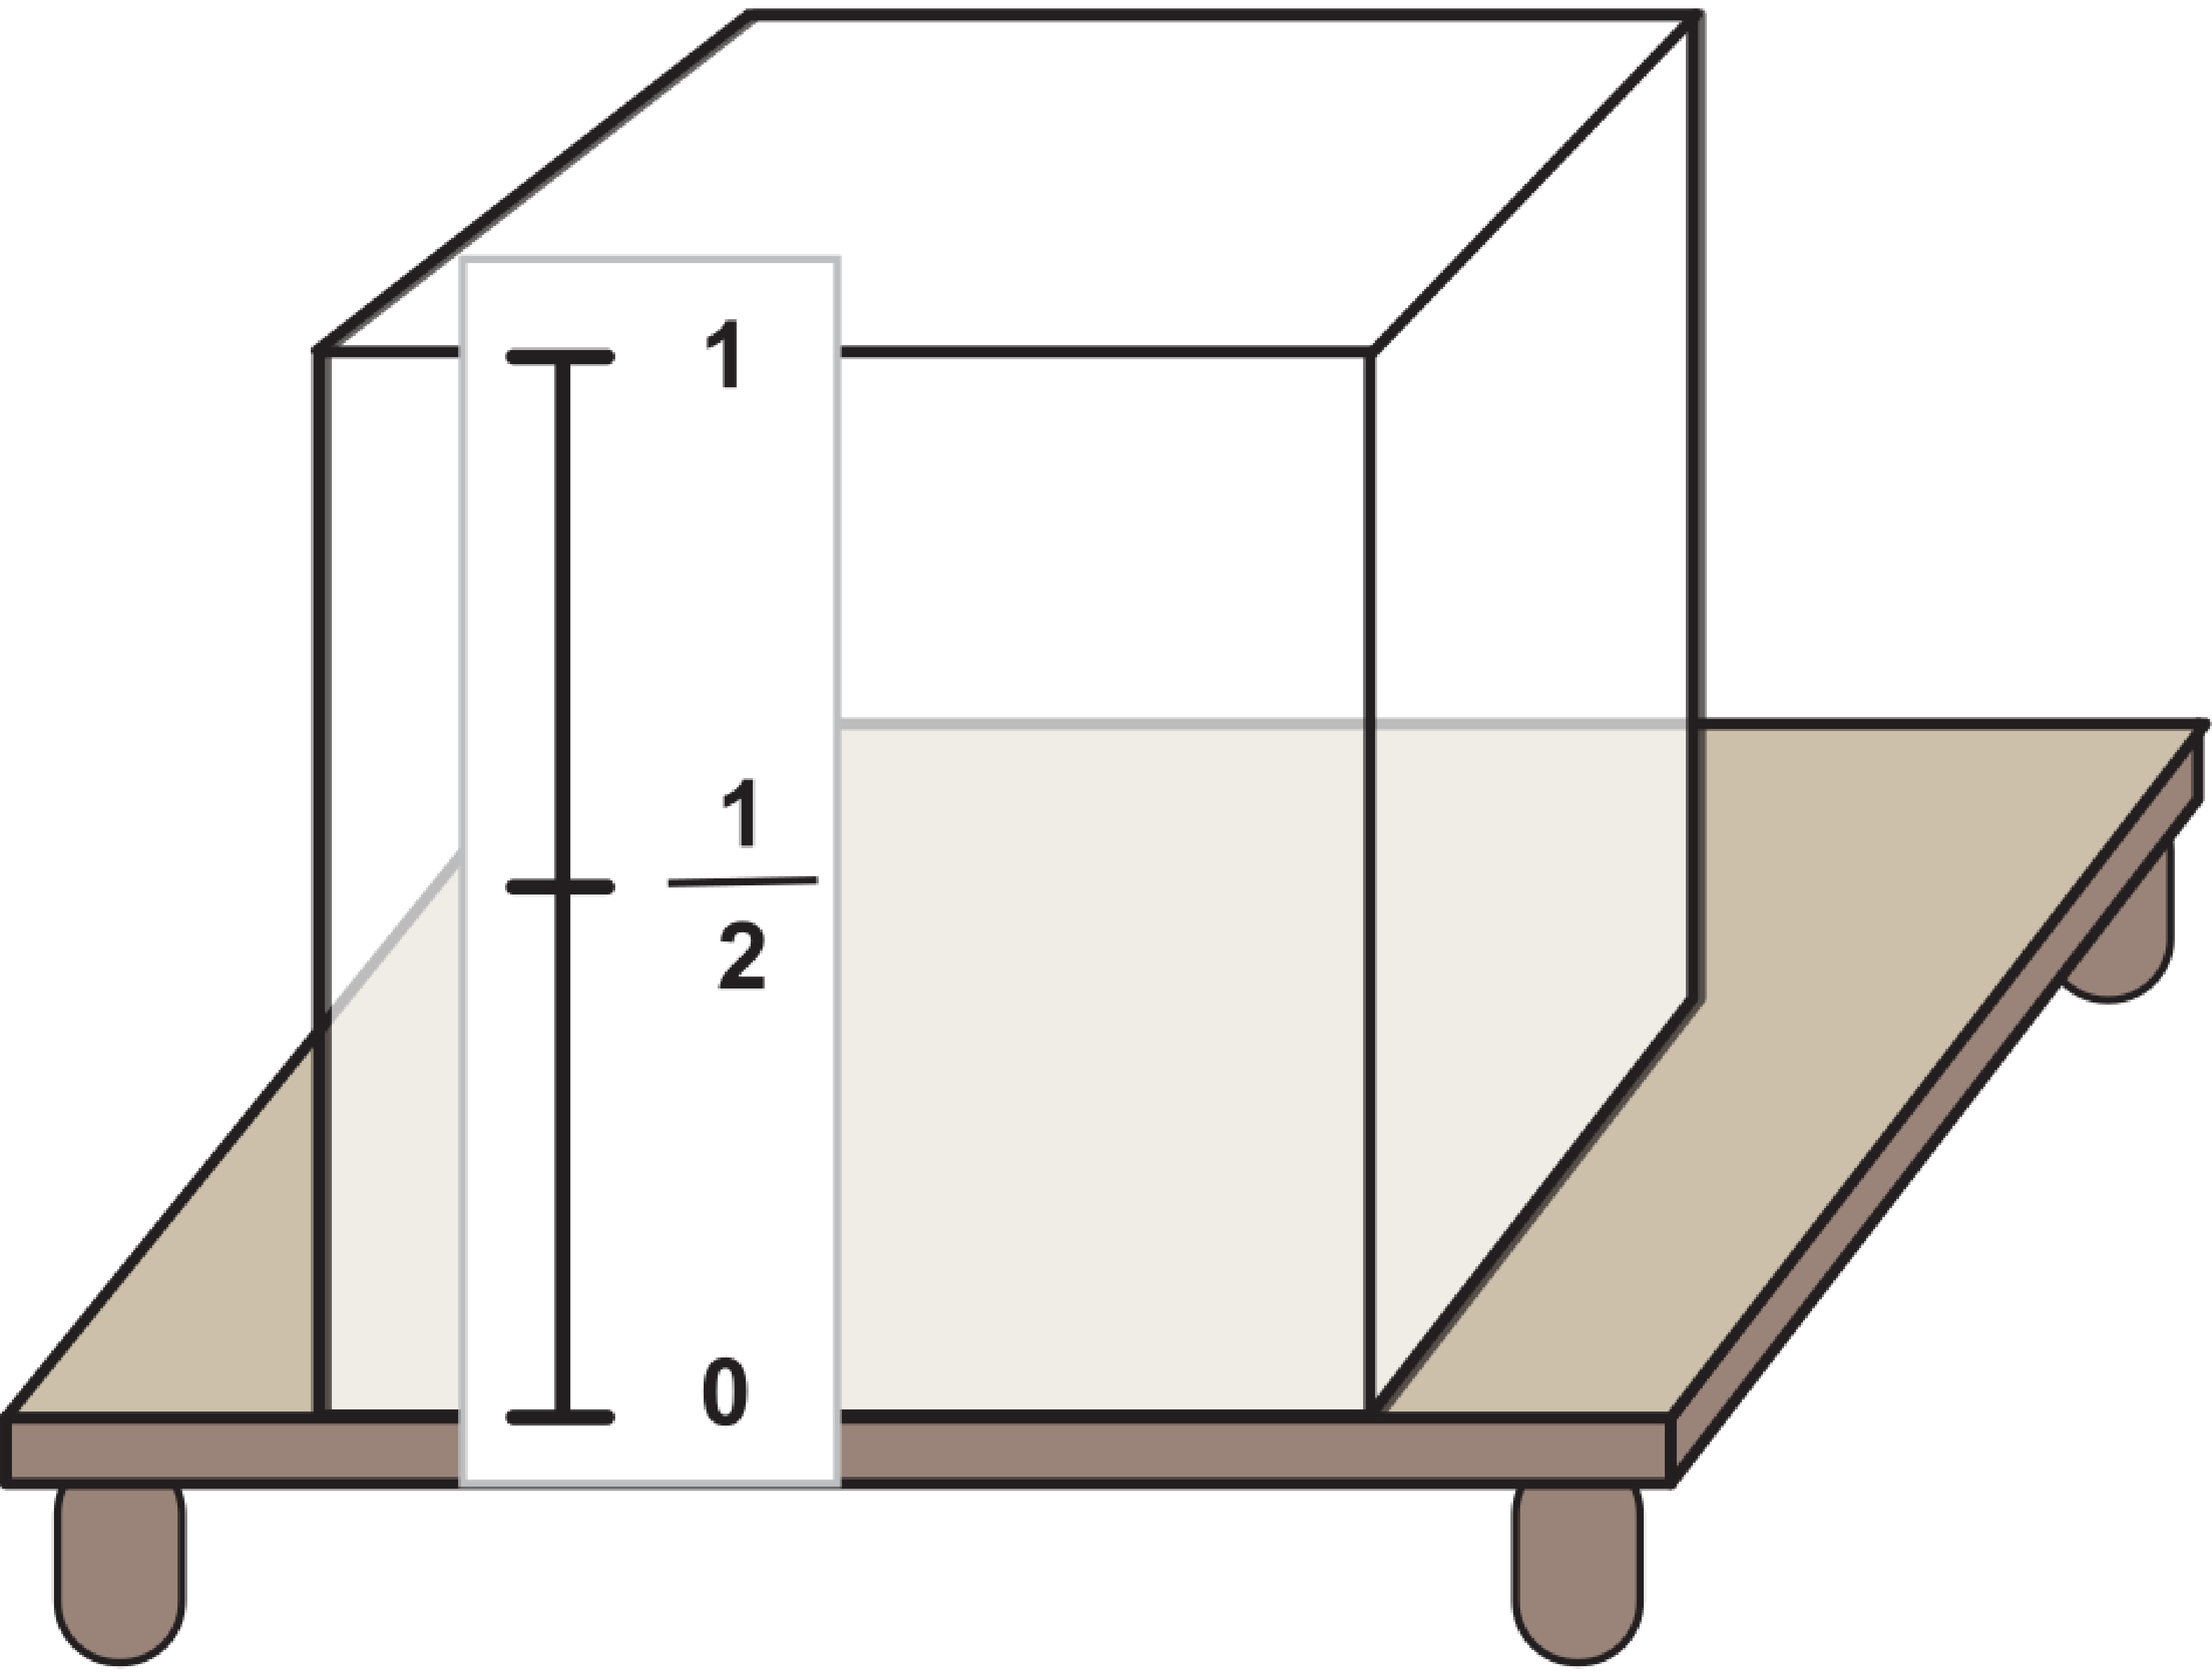
\includegraphics[width=145pt, keepaspectratio]{..//media/cap3/secoes/png/ativ1_fig09.png}
  \end{tabular}
  \end{center}

  
\subsection{Atividade}

Relembrando a representação na reta numérica: você já conhece a reta numérica com os números naturais destacados.


\begin{enumerate} [\quad a)] %s
  \item     Marque na reta numérica pontos que representem as 3 quantidades de pizza nas imagens a seguir. 

\begin{center}
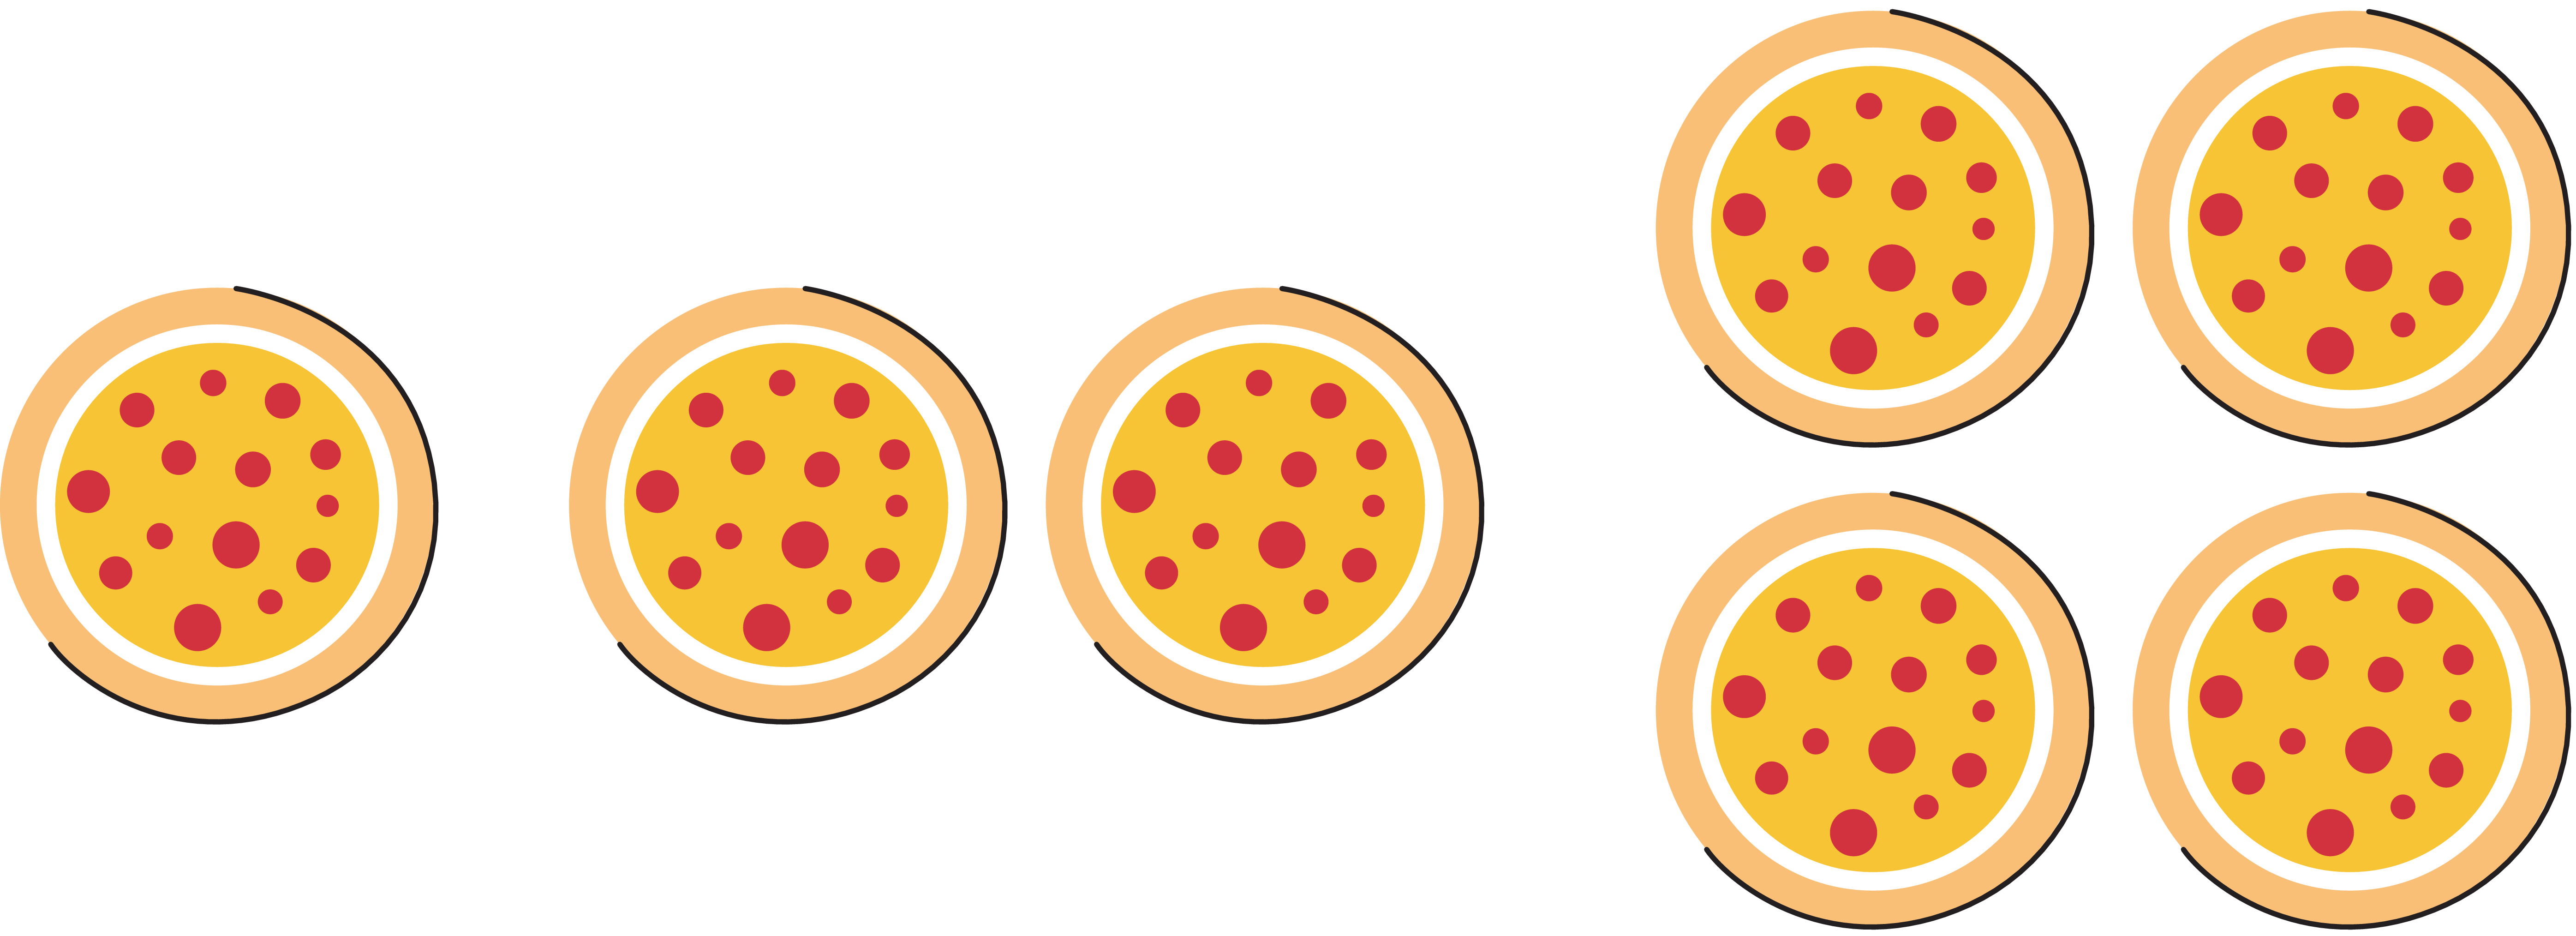
\includegraphics[width=400pt, keepaspectratio]{..//media/cap3/secoes/png/ativ2_fig_a.png} 
\end{center}

\begin{center}
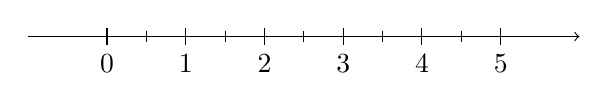
\begin{tikzpicture}[x=10mm,y=10mm]
\draw[->] (-1,0) -- (6,0) ; %edit here for the axis
\foreach \x in  {0,1,...,5} % edit here for the vertical lines
\draw[shift={(\x,0)},color=black] (0,3pt) -- (0pt,-3pt) 
node[below] {$\x$};

\foreach \x in  {0.5,1.5,...,4.5} % edit here for the vertical lines
\draw[shift={(\x,0)},color=black] (0,2pt) -- (0pt,-2pt); 

\end{tikzpicture}
\end{center}

\item     E no caso destas imagens, que pontos na reta numérica representam as 4 quantidades de pizza ilustradas?
\end{enumerate} %s

\begin{center}

\includegraphics[width=400pt, keepaspectratio]{..//media/cap3/secoes/png/ativ2_fig_b2.png} 
\end{center}


  \begin{center}
  \begin{tikzpicture}[x=30mm,y=30mm]
\draw[->] (-1/4,0) -- (2.5,0) ; %edit here for the axis
\foreach \x in  {0,0.25,...,2} % edit here for the vertical lines
\draw[shift={(\x,0)},color=black] (0,3pt) -- (0pt,-3pt); 
\foreach \x in  {0,1,2}
\draw[shift={(\x,0)},color=black] (0,3pt) -- (0pt,-3pt) node[below] {$\x$};
\end{tikzpicture}
\end{center}
  
\subsection{Atividade}

Para cada par ou trio de figuras a seguir, há uma reta numérica. Considerando a região colorida de vermelho como uma fração da figura, ligue cada uma das figuras ao número, sobre a reta numérica, correspondente à região colorida da mesma.

\begin{longtable}{lccc}
 
%retangulos 
\parbox[b][2.6cm][t]{.3cm}{a)}&
 
\begin{tikzpicture}[x=30mm,y=30mm,scale=.6]
\draw[ fill=attention] (-1.8,0) rectangle (0,1.2) node[above, shift={(-.7,0)}] {Figura 1};
\end{tikzpicture}
&&
 
\begin{tikzpicture}[x=30mm,y=30mm,scale=.6]
\draw[fill=common, fill opacity=.3] (0,0) rectangle (1.8,1.2);
\node[above, black] at (.9,1.2) {Figura 2};
\draw[fill=attention] (0,0) -- (0,1.2) --(1.8,0)--cycle;
\end{tikzpicture}
 
\\
 
\multicolumn{4}{c}{
\parbox[c][.7cm][t]{8cm}{ } }
 
\\
 
&\multicolumn{3}{c}{
\begin{tikzpicture}[x=45mm,y=45mm]
\draw[->] (-0.5,0) -- (1.5,0) ; %edit here for the axis
\foreach \x in  {0,1} % edit here for the vertical lines
\draw[shift={(\x,0)},color=black] (0,3pt) -- (0pt,-3pt) 
node[below] {$\x$};
\draw[shift={(0.5,0)},color=black] (0,3pt) -- (0pt,-3pt) 
node[below] {$\frac{1}{2}$};
\end{tikzpicture}   
}
 
\\ 
\parbox[b][2.6cm][t]{.3cm}{b)}&
 
%quadrados
 
 
 \begin{tikzpicture}[x=30mm,y=30mm]
\def\scale{.6}
%
\draw[fill=common, fill opacity=.3, scale=\scale] (-1.2,0) rectangle (0,1.2);
\draw[fill=attention, scale=\scale] (-1.2,0) rectangle (-0.8,.4);
\draw[fill=attention, scale=\scale] (-.4,0) rectangle (0,.4);
\draw[fill=attention, scale=\scale] (-1.2,0.8) rectangle (-0.8,1.2);
\draw[fill=attention, scale=\scale] (-.4,0.8) rectangle (0,1.2);
\draw[fill=attention, scale=\scale] (-.8,0.4) rectangle (-0.4,.8);

% \draw[ fill=attention, scale=\scale] (-1.2,.8) rectangle (0,1.2);
 
% \draw[fill=common, fill opacity=.3, scale=\scale] (-0.8,0) rectangle (-.4,.4);
% \draw[ fill=attention, scale=\scale] (-0.8,.4) rectangle (-0.4,.8);
% \draw[fill=common, fill opacity=.3, scale=\scale] (-0.8,.8) rectangle (-.4,1.2);
\end{tikzpicture}
&&
 \begin{tikzpicture}[x=30mm,y=30mm]
\def\scale{.6}
\draw[fill=attention, scale=\scale] (0,0) rectangle (1.2,1.2);
\end{tikzpicture}
 
\\
 
\multicolumn{4}{c}{
\parbox[c][.7cm][t]{8cm}{ } }
 
\\
 
&\multicolumn{3}{c}{
\begin{tikzpicture}[x=45mm,y=45mm]
\draw[->] (-0.5,0) -- (1.5,0) ; %edit here for the axis
\foreach \x in  {0,0.1111,...,1}{ % edit here for the vertical lines
\draw[shift={(\x,0)},color=black] (0,3pt) -- (0pt,-3pt);} 
\foreach \x in  {0,1}
\draw[shift={(\x,0)},color=black] (0,3pt) -- (0pt,-3pt) node[below] {$\x$};
\foreach \x in  {3,5}
\draw[shift={(\x/9,0)},color=black] (0,3pt) -- (0pt,-3pt) node[below] {$\frac{\x}{9}$};
\end{tikzpicture}}
\\ 
 
%hexagonos
\parbox[b][2.6cm][t]{.3cm}{c)}&
 
\begin{tikzpicture}[x=30mm,y=30mm]
\def\scale{.6}% to rescale the polygons only.
 
%hexagon on the left
\fill[shift={(0,0.6)}, fill=attention, scale=\scale] (0,0) -- (90:0.7) -- (150:0.7)-- (210:.7);
\fill[shift={(0,0.6)}, fill=common, fill opacity=.3, scale=\scale] (0,0) -- (90:0.7) -- (30:0.7)-- (-30:.7) -- (-90:.7) -- (-150:.7)--cycle;
\foreach \x in {30,90,...,330}{
\draw[shift={(0,0.6)}, scale=\scale] (\x:0.7) -- (\x + 60: 0.7);
\draw[shift={(0,0.6)}, scale=\scale] (0,0) -- (\x:0.7);}
\end{tikzpicture}
&&
\begin{tikzpicture}[x=30mm,y=30mm] 
\def\scale{.6}% to rescale the polygons only.
 
%hexagon on the right
\foreach \x in {30,90,...,330}{
\draw[shift={(1,0.6)}, fill=attention,attention, scale=\scale] (\x:0.7) -- (\x + 60: 0.7) --(0,0) --cycle;
\draw[shift={(1,0.6)}, fill=attention, scale=\scale] (\x:0.7) -- (\x + 60: 0.7);}
\end{tikzpicture}
 
\\
 
\multicolumn{4}{c}{
\parbox[c][.7cm][t]{8cm}{ } }
 
\\
&\multicolumn{3}{c}{
\begin{tikzpicture}[x=68mm,y=68mm]
\draw[->] (-1/6,0) -- (1+1/6,0) ; %edit here for the axis
\foreach \x in  {0,0.1667,...,1}{ % edit here for the vertical lines
\draw[shift={(\x,0)},color=black] (0,3pt) -- (0pt,-3pt);} 
\foreach \x in  {0,1}
\draw[shift={(\x,0)},color=black] (0,3pt) -- (0pt,-3pt) node[below] {$\x$};
\foreach \x in  {1,2}
\draw[shift={(\x/3,0)},color=black] (0,3pt) -- (0pt,-3pt) node[below] {$\frac{\x}{3}$};
\end{tikzpicture} }
\\ 
 
\parbox[b][2.6cm][t]{.3cm}{d)}&
 
 %triangulos
\begin{tikzpicture}[x=30mm,y=30mm]
\def\scale{.6}% to rescale the polygons only.
 
\foreach \x in {90,210,330}{
\draw[attention,fill=attention, shift={(0,0.6)}, scale=\scale] (\x:0.7) -- (\x + 120: 0.7) -- (0,0)--cycle;
\draw[shift={(0,0.6)}, scale=\scale] (\x:0.7) -- (\x + 120: 0.7);}
\draw[shift={(0,0.6)}, scale=\scale] (-90:0.35) -- (30: 0.35) -- (150: 0.35) -- cycle;
\end{tikzpicture}
&&
\begin{tikzpicture}[x=30mm,y=30mm]
\def\scale{.6}% to rescale the polygons only.
\fill[shift={(1,0.6)}, scale=\scale, common, fill opacity=.3] (90:0.7) -- (210: 0.7)--(330:.7)--cycle;
\foreach \x in {90,210,330}{
\draw[shift={(1,0.6)}, scale=\scale] (\x:0.7) -- (\x + 120: 0.7);}
\draw[fill=attention, shift={(1,0.6)}, scale=\scale] (-90:0.35) -- (30: 0.35) -- (150: 0.35) -- cycle;
\end{tikzpicture}
 
\\
 
\multicolumn{4}{c}{
\parbox[c][.7cm][t]{8cm}{ } }
 
\\
&\multicolumn{3}{c}{
\begin{tikzpicture}[x=60mm,y=60mm]
\draw[->] (-1/4,0) -- (1+1/4,0) ; %edit here for the axis
\foreach \x in  {0,0.25,...,1}{ % edit here for the vertical lines
\draw[shift={(\x,0)},color=black] (0,3pt) -- (0pt,-3pt);} 
\foreach \x in  {0,1}
\draw[shift={(\x,0)},color=black] (0,3pt) -- (0pt,-3pt) node[below] {$\x$};
\foreach \x in  {1,3}
\draw[shift={(\x/4,0)},color=black] (0,3pt) -- (0pt,-3pt) node[below] {$\frac{\x}{4}$};
\end{tikzpicture}}
\\
 
\parbox[b][2.6cm][t]{.3cm}{e)}&
 
%os baianos e os novos retangulos
\begin{tikzpicture} [x=30mm,y=30mm]
\def\scalefig {.6}
\draw[shift={(-.35*\scalefig,0.3)}, fill=attention, scale=\scalefig] (-1.5,0) rectangle (-0.5,1.2) node[above, shift={(-.25*\scalefig,0)}] {Figura 1};
\draw[shift={(-.35*\scalefig,0.3)}, scale=\scalefig, fill=common, fill opacity=.3] (-.5,0) rectangle (0,1.2);
\draw[shift={(-.35*\scalefig,0.3)}, scale=\scalefig] (-1,0) -- (-1,1.2);
\end{tikzpicture}
&
\begin{tikzpicture} [x=30mm,y=30mm] 
\def\scalefig {.6}
\draw[shift={(1.25*\scalefig,0.3)}, fill=attention, scale=\scalefig] (-1.5,0) rectangle (-1,1.2);
\draw[shift={(1.25*\scalefig,0.3)}, scale=\scalefig, fill=common, fill opacity=.3] (-1,0) rectangle (0,1.2); 
\node[shift={(1.25*\scalefig,0.3)}] at (-.48,.85) {Figura 2};
\draw[shift={(1.25*\scalefig,0.3)}, scale=\scalefig] (-.5,0) -- (-.5,1.2);
\end{tikzpicture}
&
\begin{tikzpicture} [x=30mm,y=30mm] 
\def\scalefig {.6}
\draw[shift={(1.35*\scalefig,0.3)}, fill=attention, scale=\scalefig] (0,0) rectangle (1.5,1.2) node[above, shift={(-.75*\scalefig,0)}] {Figura 3};
\draw[shift={(1.35*\scalefig,0.3)}, scale=\scalefig] (.5,0) -- (.5,1.2);
\draw[shift={(1.35*\scalefig,0.3)}, scale=\scalefig] (1,0) -- (1,1.2);
\end{tikzpicture}
 
\\
 
\multicolumn{4}{c}{
\parbox[c][.7cm][t]{8cm}{ } }
 
\\
&\multicolumn{3}{c}{
\begin{tikzpicture}[x=55mm,y=55mm]
 \begin{scope}[shift={(-.3,0)}]
\draw[->] (-1/3,0) -- (1.33,0) ; %edit here for the axis
\foreach \x in  {0,1} % edit here for the vertical lines
\draw[shift={(\x,0)},color=black] (0,3pt) -- (0pt,-3pt) 
node[below] {$\x$};
\foreach \x in {1,2}
\draw[shift={(\x/3,0)},color=black] (0,3pt) -- (0pt,-3pt) 
node[below] {$\frac{\x}{3}$};
\end{scope}
\end{tikzpicture}}
\\
\parbox[b][2.6cm][t]{.3cm}{f)}&
 
\begin{tikzpicture}[scale=.48]
\fill[common, fill opacity=.3] (0,0) rectangle (45,45); 
 \fill[attention] (0,33.75) rectangle (33.75,45);
 \draw[step=11.25, fill=attention] (0,0) grid (45,45); 
\end{tikzpicture}
&
\begin{tikzpicture}[scale=.48]
\draw[fill=attention] (0,0) rectangle (45,45);
\end{tikzpicture}
&
 
\begin{tikzpicture}[scale=.48]
  \draw[step=11.25, fill=attention] (0,0) rectangle (45,45); 
  \draw[step=11.25, fill=white] (11.25,0) rectangle (45,11.25);
  \draw[step=11.25, fill=common, fill opacity=.3] (11.25,0) rectangle (45,11.25);
  \draw[step=11.25] (0,0) grid (45,45); 
\end{tikzpicture}
\\
 
\multicolumn{4}{c}{
\parbox[c][.7cm][t]{8cm}{ } }
 
\\
&\multicolumn{3}{c}{
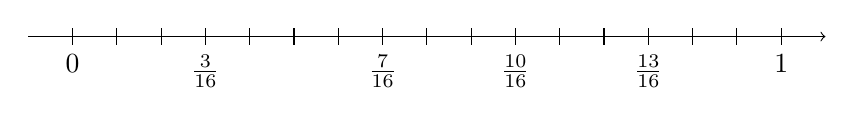
\begin{tikzpicture}[x=90mm,y=90mm]
 \draw[->] (-1/16,0) -- (1+1/16,0) ; %edit here for the axis
 \foreach \x in  {0,0.0625,...,1}{ % edit here for the vertical lines
 \draw[shift={(\x,0)},color=black] (0,3pt) -- (0pt,-3pt);} 
\foreach \x in  {0,1}
\draw[shift={(\x,0)},color=black] (0,3pt) -- (0pt,-3pt) node[below] {$\x$};
\foreach \x in  {3,7,10,13}
\draw[shift={(\x/16,0)},color=black] (0,3pt) -- (0pt,-3pt) node[below] {$\frac{\x}{16}$};
\end{tikzpicture}
}
\end{longtable}

\subsection{Atividade}

Para cada uma das figuras a seguir, marque na reta numérica o ponto correspondente à fração da unidade destacada na imagem:


\begin{enumerate} [\quad a)] %s
  \item     A unidade é uma pizza. 

\begin{center}
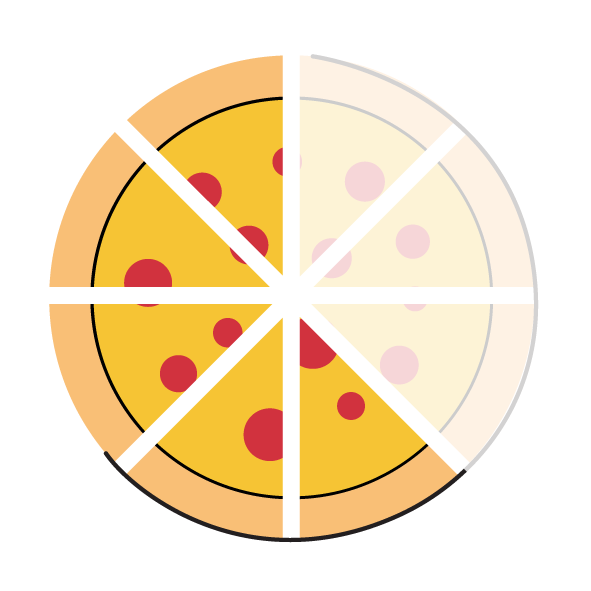
\includegraphics[width=60pt, keepaspectratio]{..//media/cap3/secoes/png/ativ4_fig_a.png} 
\quad\quad\quad \begin{tikzpicture}[x=56.25mm,y=56.25mm]
\draw[->] (-0.3,0) -- (1.3,0) ; %edit here for the axis
\foreach \x in  {0,1} % edit here for the vertical lines
\draw[shift={(\x,0)},color=black] (0,3pt) -- (0pt,-3pt) 
node[below] {$\x$};
 
\foreach \x in {3,5}
\draw[shift={(\x/8,0)},color=black] (0,3pt) -- (0pt,-3pt) 
node[below] {$\frac{\x}{8}$};
\end{tikzpicture}   
\end{center}

\item     A unidade é uma barra de chocolate. 

\begin{center}
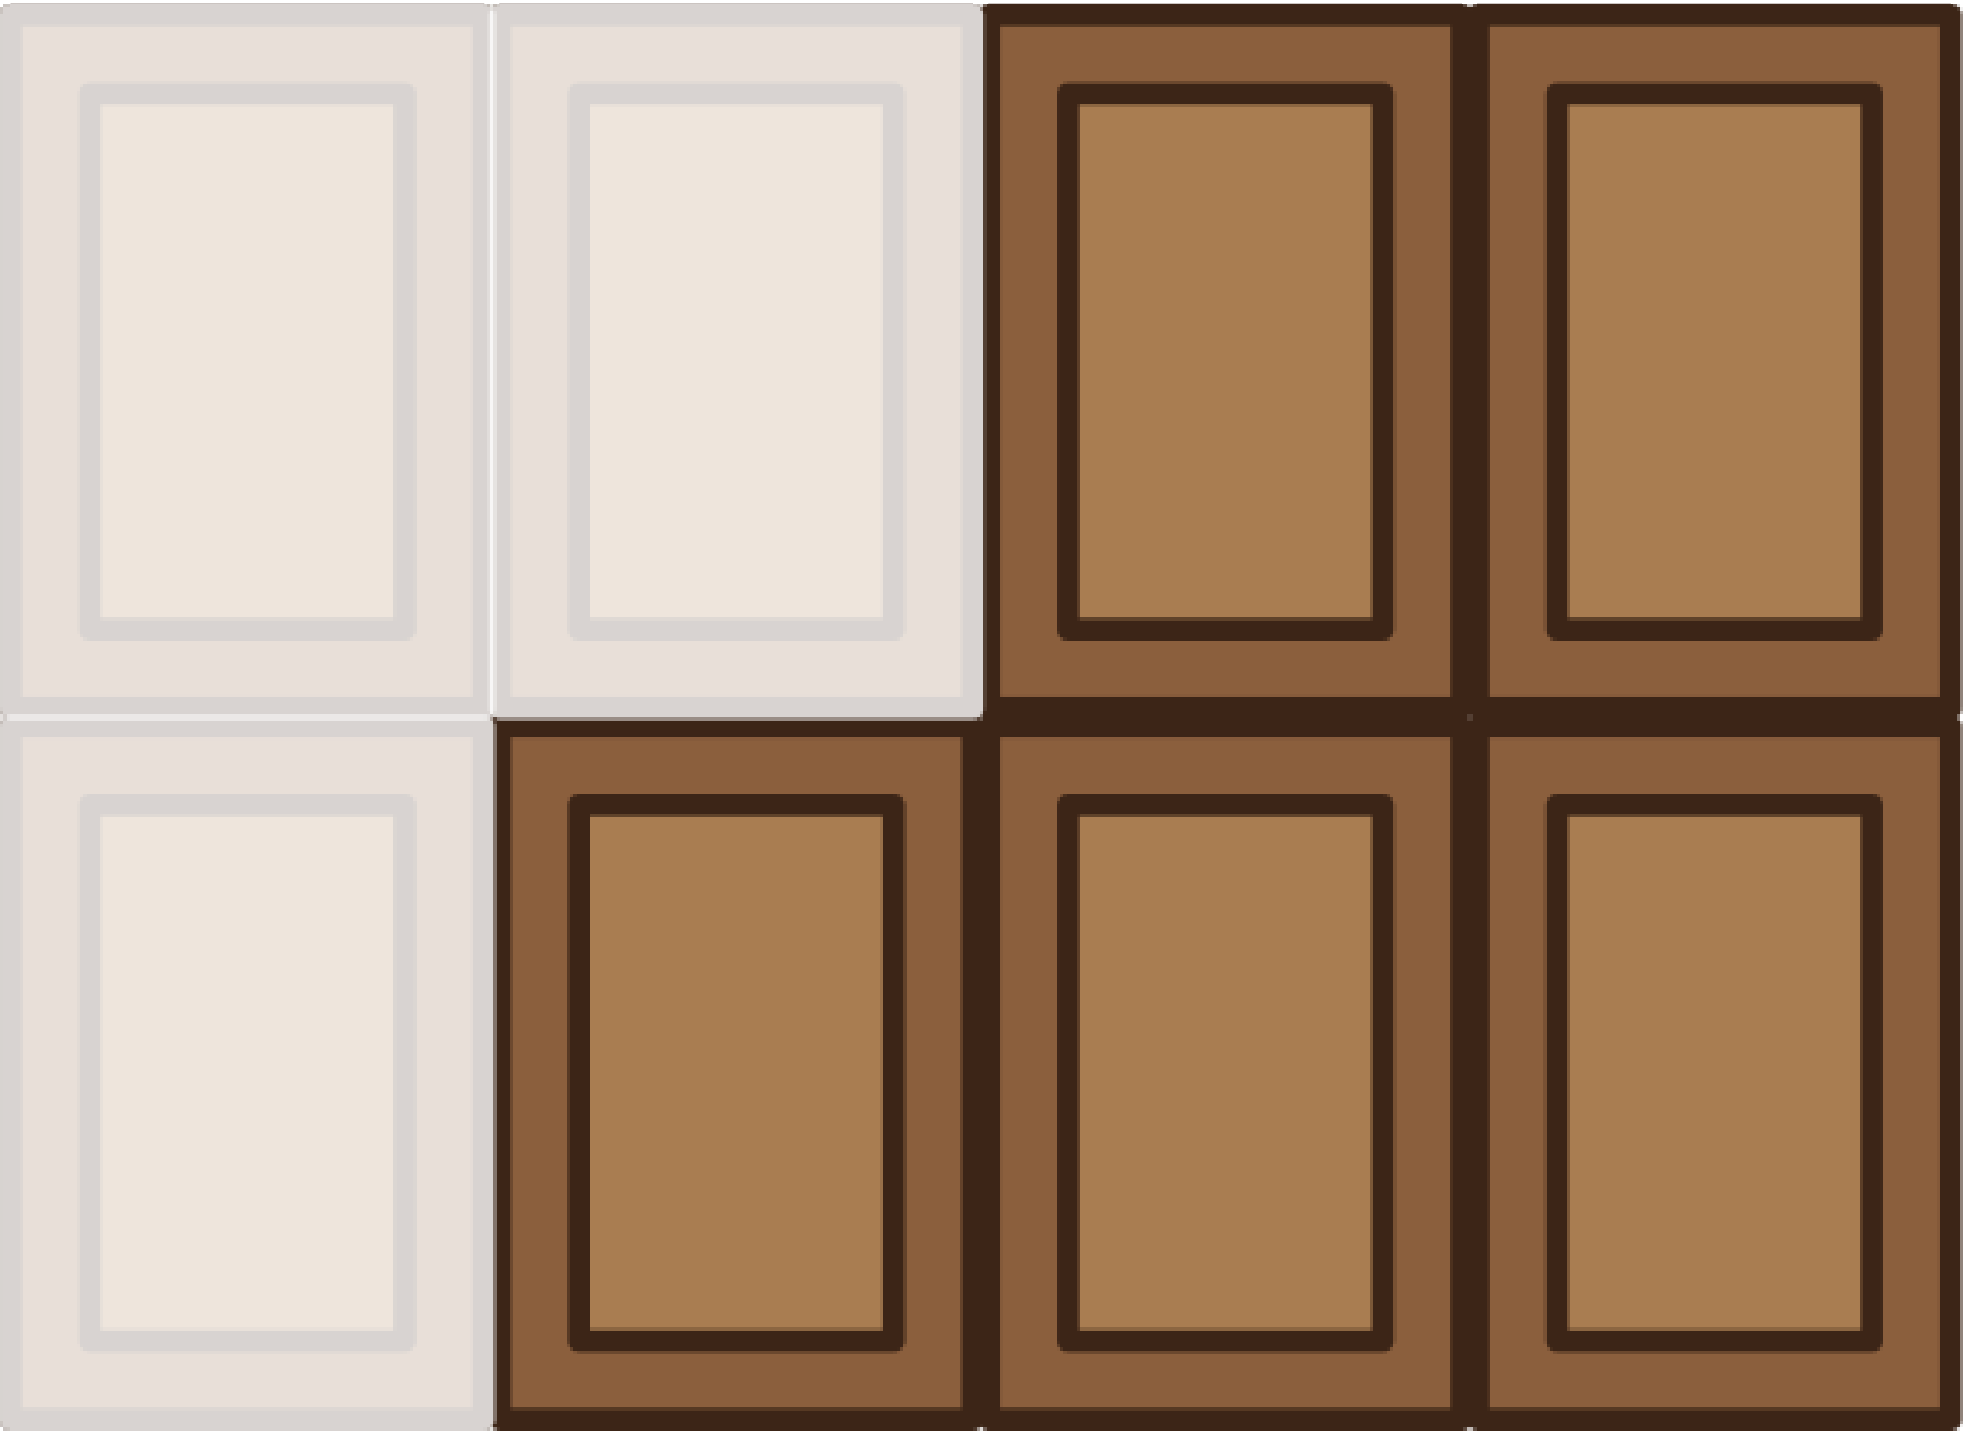
\includegraphics[width=100pt, keepaspectratio]{..//media/cap3/secoes/png/ativ4_fig_b.png} \quad \quad \quad
\begin{tikzpicture}[x=56.25mm,y=56.25mm]
\draw[->] (-0.3,0) -- (1.3,0) ; %edit here for the axis
\foreach \x in  {0,1} % edit here for the vertical lines
\draw[shift={(\x,0)},color=black] (0,3pt) -- (0pt,-3pt) 
node[below] {$\x$};
 
\foreach \x in {3,5}
\draw[shift={(\x/8,0)},color=black] (0,3pt) -- (0pt,-3pt) 
node[below] {$\frac{\x}{8}$};
\end{tikzpicture}   
\end{center}

\item     A unidade é uma maçã. 

\begin{center}

\includegraphics[width=80pt, keepaspectratio]{..//media/cap3/secoes/png/ativ4_fig_c.png} \quad \quad \quad
\begin{tikzpicture}[x=60mm,y=60mm]
\draw[->] (-1/4,0) -- (1+1/4,0) ; %edit here for the axis
\foreach \x in  {0,0.25,...,1}{ % edit here for the vertical lines
\draw[shift={(\x,0)},color=black] (0,3pt) -- (0pt,-3pt);} 
\foreach \x in  {0,1}
\draw[shift={(\x,0)},color=black] (0,3pt) -- (0pt,-3pt) node[below] {$\x$};
\foreach \x in  {1,3}
\draw[shift={(\x/4,0)},color=black] (0,3pt) -- (0pt,-3pt) node[below] {$\frac{\x}{4}$};
\draw[shift={(.5,0)},color=black] (0,3pt) -- (0pt,-3pt) node[below] {$\frac{1}{2}$};
\end{tikzpicture}
\end{center}

  \item     A unidade é um sanduíche de queijo com presunto. 

\begin{center}
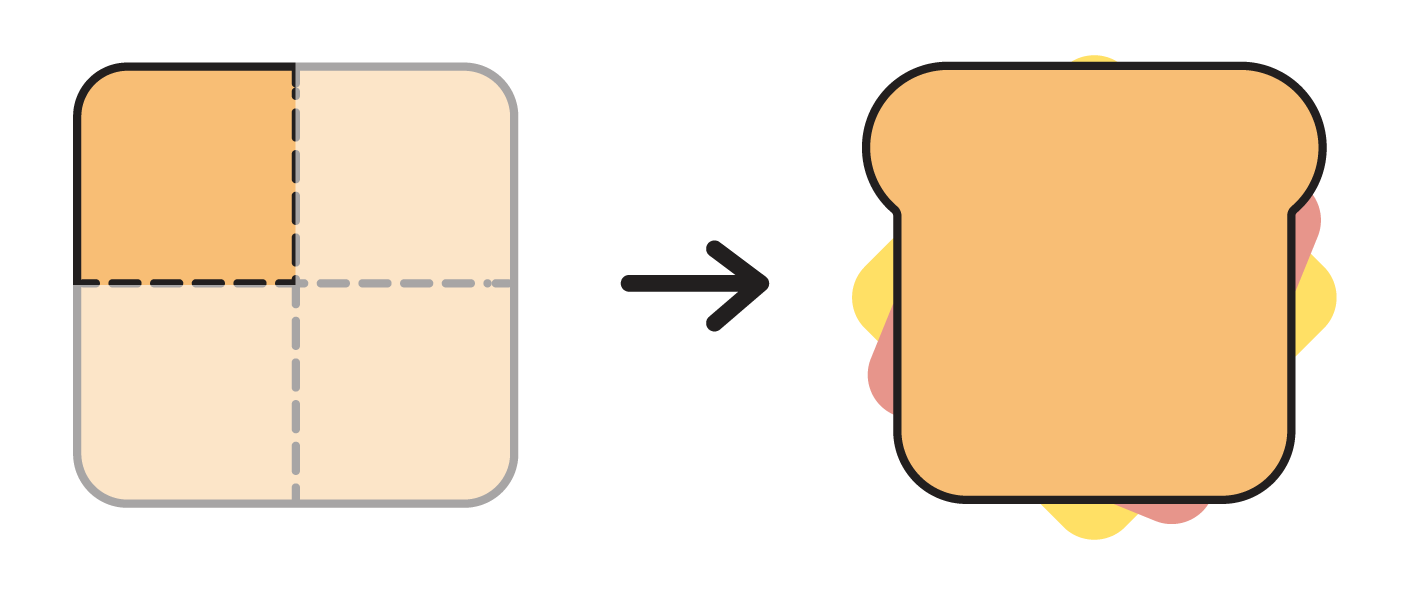
\includegraphics[width=100pt, keepaspectratio]{..//media/cap3/secoes/png/ativ4_fig_d.png} \quad \quad \quad
\begin{tikzpicture}[x=60mm,y=60mm]
\draw[->] (-1/4,0) -- (1+1/4,0) ; %edit here for the axis
\foreach \x in  {0,0.25,...,1}{ % edit here for the vertical lines
\draw[shift={(\x,0)},color=black] (0,3pt) -- (0pt,-3pt);} 
\foreach \x in  {0,1}
\draw[shift={(\x,0)},color=black] (0,3pt) -- (0pt,-3pt) node[below] {$\x$};
\foreach \x in  {1,3}
\draw[shift={(\x/4,0)},color=black] (0,3pt) -- (0pt,-3pt) node[below] {$\frac{\x}{4}$};
\draw[shift={(.5,0)},color=black] (0,3pt) -- (0pt,-3pt) node[below] {$\frac{1}{2}$};
\end{tikzpicture}
\end{center}

\item A unidade é uma torta. 

\begin{center}
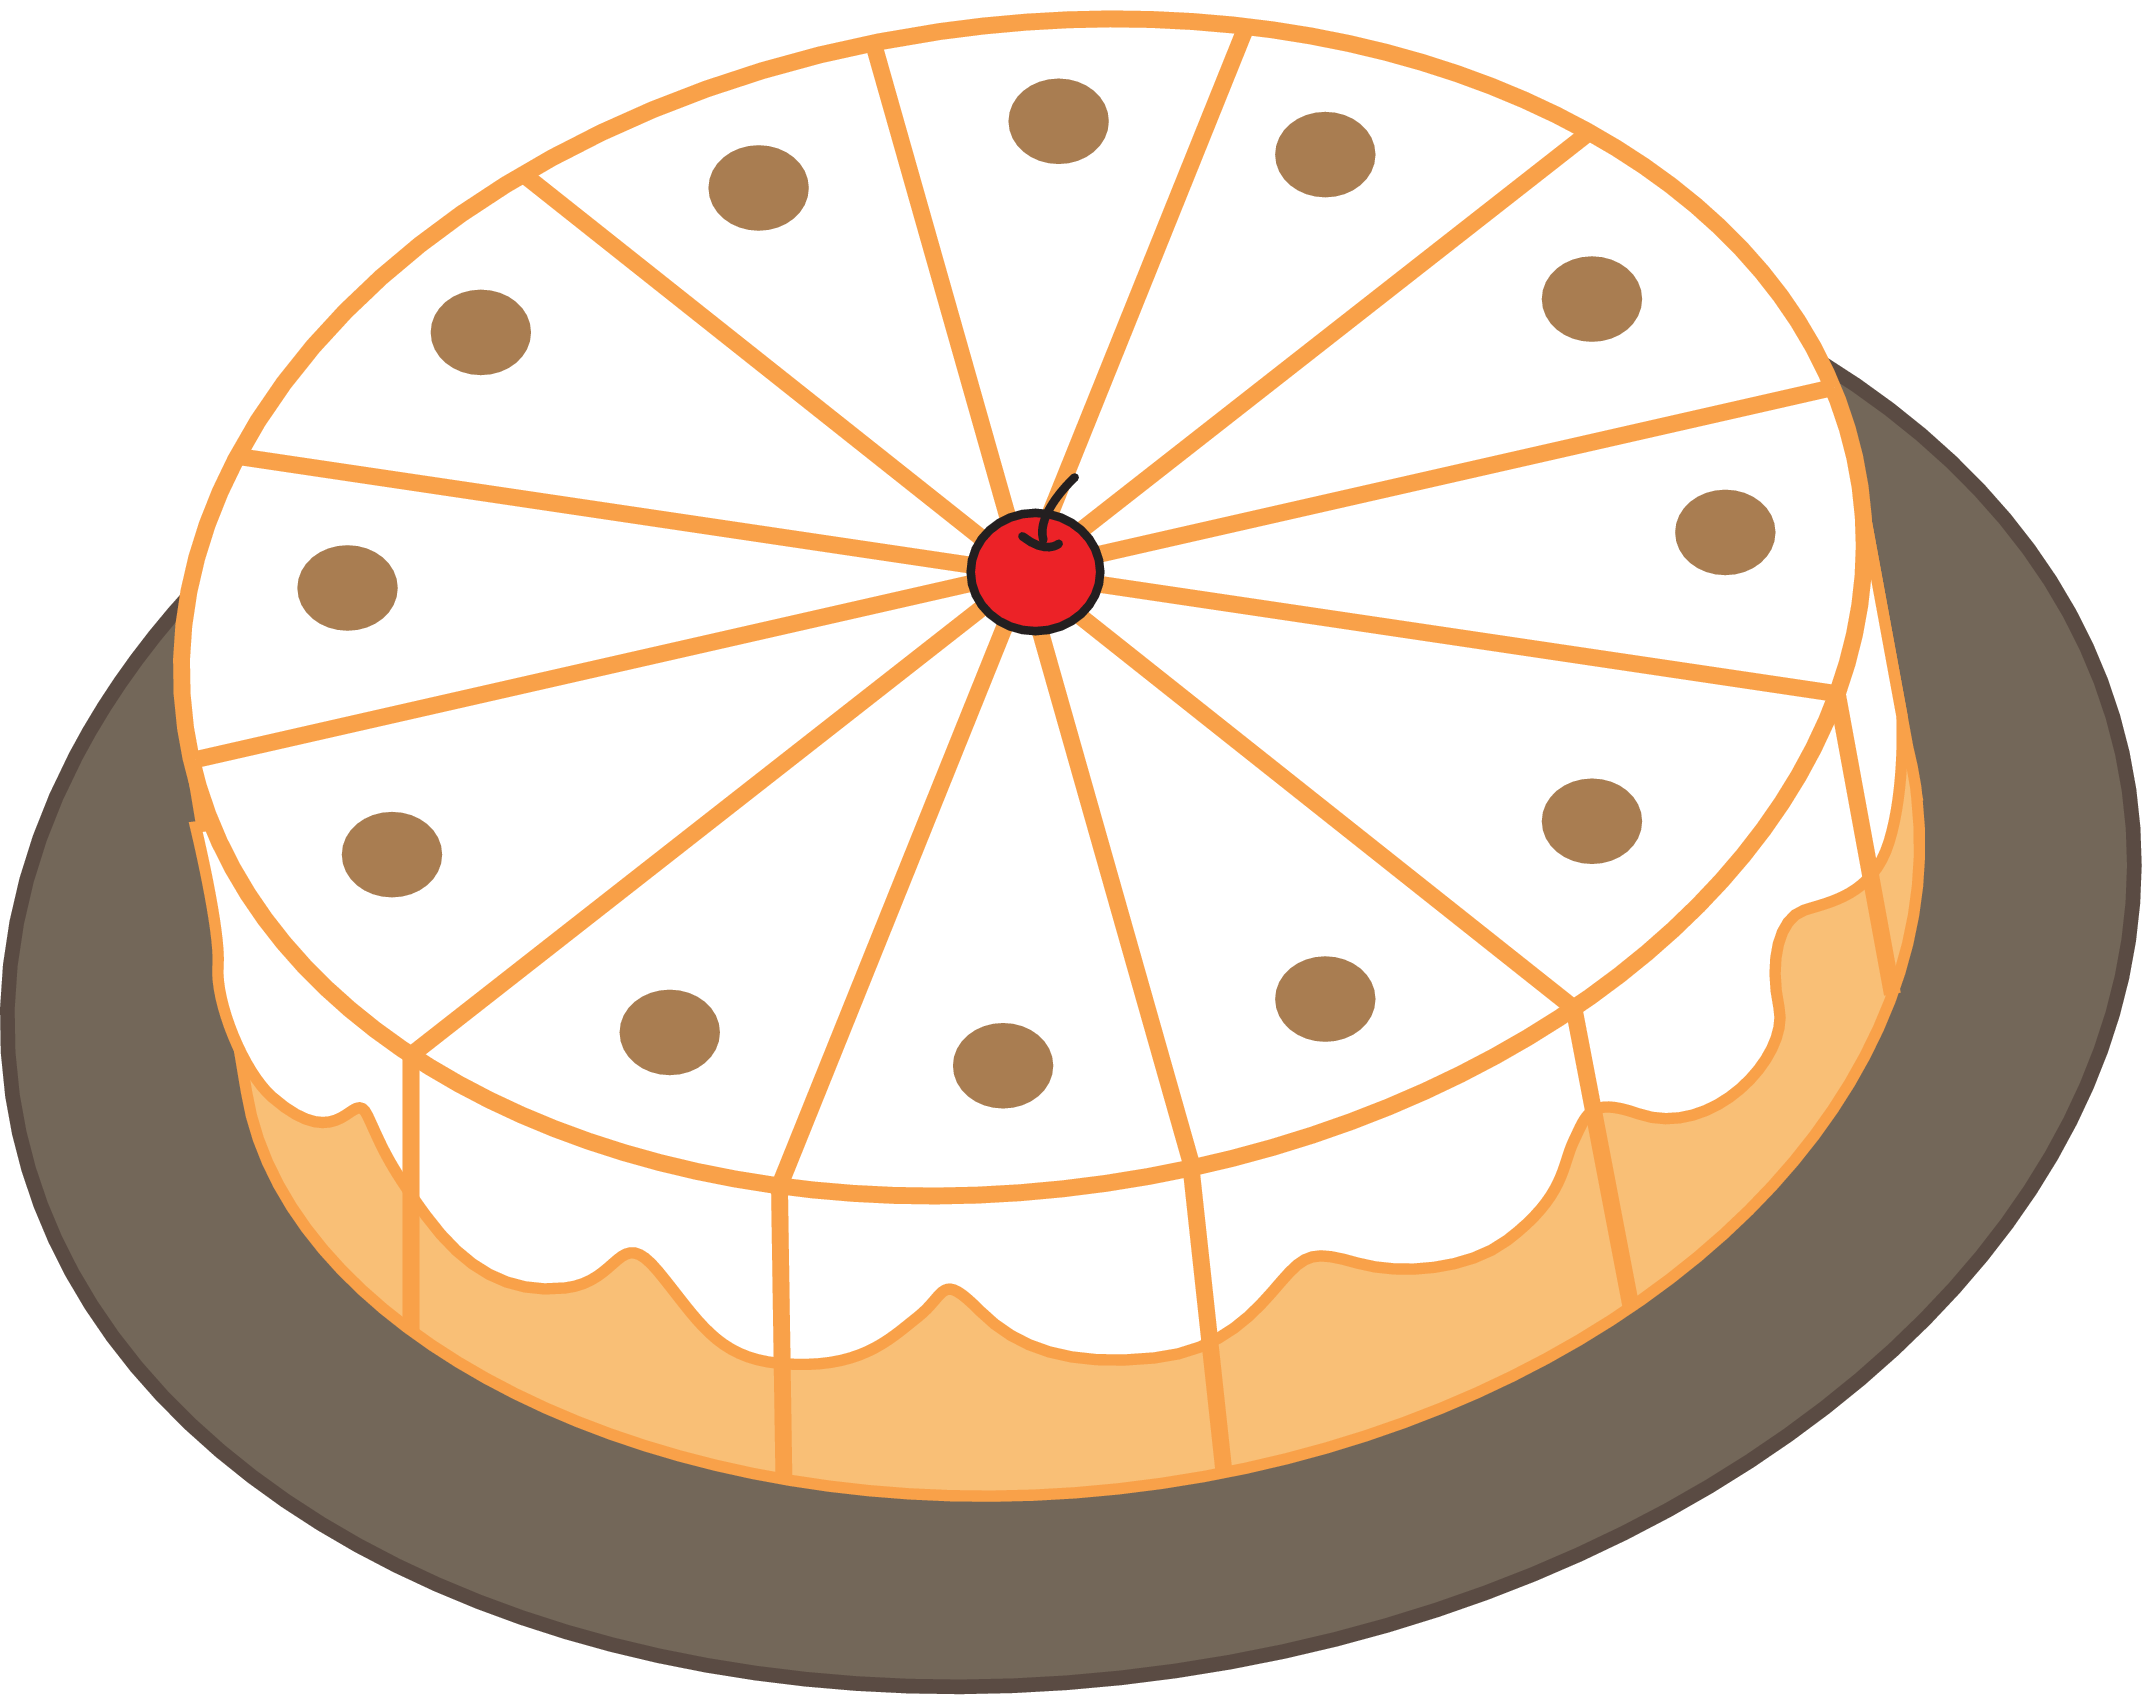
\includegraphics[width=100pt, keepaspectratio]{..//media/cap3/secoes/png/ativ4_fig_e.png} \quad \quad \quad
 \begin{tikzpicture}[x=25.71mm,y=25.71mm]
\draw[->] (-.5,0) -- (3,0) ; %edit here for the axis
\foreach \x in  {0,0.5,...,2.5}{ % edit here for the vertical lines
\draw[shift={(\x,0)},color=black] (0,3pt) -- (0pt,-3pt);} 
\foreach \x in  {0,1,2}
\draw[shift={(\x,0)},color=black] (0,3pt) -- (0pt,-3pt) node[below] {$\x$};
\foreach \x in  {1,3,5}
\draw[shift={(\x/2,0)},color=black] (0,3pt) -- (0pt,-3pt) node[below] {$\frac{\x}{2}$};
\end{tikzpicture}
\end{center}

  \item     A unidade é um biscoito. 

\begin{center}

\includegraphics[width=100pt, keepaspectratio]{..//media/cap3/secoes/png/ativ4_fig_f.png} \quad \quad \quad
\begin{tikzpicture}[x=25.71mm,y=25.71mm]
\draw[->] (-.5,0) -- (3,0) ; %edit here for the axis
\foreach \x in  {0,0.5,...,2.5}{ % edit here for the vertical lines
\draw[shift={(\x,0)},color=black] (0,3pt) -- (0pt,-3pt);} 
\foreach \x in  {0,1,2}
\draw[shift={(\x,0)},color=black] (0,3pt) -- (0pt,-3pt) node[below] {$\x$};
\foreach \x in  {1,3,5}
\draw[shift={(\x/2,0)},color=black] (0,3pt) -- (0pt,-3pt) node[below] {$\frac{\x}{2}$};
\end{tikzpicture}
\end{center}

  \item     A unidade é um copo cheio. 
\end{enumerate} %s

\begin{flushright}
 \begin{tabular}{rcr}

\includegraphics[width=50pt, keepaspectratio]{..//media/cap3/secoes/png/ativ4_fig_g.png}  & \quad\quad\quad\quad&
 \begin{tikzpicture}[x=25.71mm,y=25.71mm]
\draw[->] (-.5,0) -- (3,0) ; %edit here for the axis
\foreach \x in  {0,0.5,...,2.5}{ % edit here for the vertical lines
\draw[shift={(\x,0)},color=black] (0,3pt) -- (0pt,-3pt);} 
\foreach \x in  {0,1,2}
\draw[shift={(\x,0)},color=black] (0,3pt) -- (0pt,-3pt) node[below] {$\x$};
\foreach \x in  {1,3,5}
\draw[shift={(\x/2,0)},color=black] (0,3pt) -- (0pt,-3pt) node[below] {$\frac{\x}{2}$};
\end{tikzpicture}
\end{tabular}
\end{flushright}


\subsection{Atividade}

A faixa a seguir está dividida em 5 partes iguais. 

\begin{center}
 \begin{tikzpicture}[x=56.25mm,y=56.25mm]
\foreach \x in {0,1,2,...,4}{
\draw[fill=common, fill opacity=.3] (\x/5,0) rectangle (\x/5 + 1/5,.1);
\draw[step=.2] (0,0) grid (1,.1);
\draw (0,.1)-- (1,.1);}
 \end{tikzpicture}
\end{center}


\begin{enumerate} [\quad a)] %s
  \item     Considerando a faixa como unidade, escreva na reta numérica a fração correspondente a cada uma das regiões coloridas de vermelho.


\begin{center}
\begin{tikzpicture}[x=56.25mm,y=56.25mm]
\foreach \x in {1,2,...,5}{
\fill[fill=common, fill opacity=.3, shift={(0,-\x*.15)}] (\x/5,0) rectangle (1,.1);
\draw[fill=attention, shift={(0,-\x*.15)}] (0,0) rectangle (\x/5,.1);
\draw[step=.2, shift={(0,-\x*.15)}] (0,0) grid (1,.1);
\draw[shift={(0,-\x*.15)}] (0,.1)-- (1,.1);}
 
\begin{scope}[shift={(0,-.9)}]
\draw[->] (-0.1,0) -- (1.1,0) ; %edit here for the axis
\foreach \x in  {0,1} % edit here for the vertical lines
\draw[shift={(\x,0)},color=black] (0,3pt) -- (0pt,-3pt) node[below] {$\x$};
 
\foreach \x in  {.2,.4,.6,.8} % edit here for the vertical lines
\draw[shift={(\x,0)},color=black] (0,3pt) -- (0pt,-3pt) node[below] {{\Large $\frac{\square}{\square}$}};
\end{scope}

\end{tikzpicture}   
 \end{center}
 
  \item     Escreva, em linguagem simbólica, a fração correspondente à faixa inteira. De que outra maneira é possível indicar essa quantidade? 

\end{enumerate} %s


\subsection{Atividade}

A professora Julia pediu que os seus alunos, Pedro e Miguel, marcassem $\frac{1}{2}$ na reta numérica traçada em uma fita, como esta que vocês também receberam:

\begin{center}
 \begin{tikzpicture}[x=56.25mm,y=56.25mm]
\draw[fill=common, fill opacity=.3] (0,-.15) rectangle (1.2,.15);
\draw (0,0) -- (1.2,0) ; %edit here for the axis
\draw (1,3pt) -- (1,-3pt) node[below] {1};
\node at (.03,-.05) {0};
\end{tikzpicture} 
\end{center}

Pedro trouxe a seguinte marcação: 
 \begin{tikzpicture}[x=56.25mm,y=56.25mm]
\draw[fill=common, fill opacity=.3] (0,-.15) rectangle (1.2,.15);
\draw (0,0) -- (1.2,0) ; %edit here for the axis
\draw[dashed] (0.6,-.15) -- (.6,.15);
\draw (1,3pt) -- (1,-3pt) node[below] {1};
\node at (.03,-.05) {0};
\node at (.63,-.05) {$\frac{1}{2}$};
\end{tikzpicture}

Miguel trouxe esta:
 \begin{tikzpicture}[x=56.25mm,y=56.25mm]
\draw[fill=common, fill opacity=.3] (0,-.15) rectangle (1.2,.15);
\draw (0,0) -- (1.2,0) ; %edit here for the axis
\draw[dashed] (0.5,-.15) -- (.5,.15);
\draw (1,3pt) -- (1,-3pt) node[below] {1};
\node at (.03,-.05) {0};
\node at (.53,-.05) {$\frac{1}{2}$};
\end{tikzpicture} 

\begin{enumerate} [\quad a)] %s
  \item     É possível ambos estarem corretos? Justifique sua resposta. 
  \item     Faça marcações correspondentes a     $\frac{1}{4}$     e a     $\frac{3}{4}$  na reta numérica desenhada na fita. Explique como você fez essas marcações.
  \item     Onde deve ser feita a marcação correspondente a     $\frac{4}{4}$    ? 
  \item     E a marcação correspondente a     $\frac{5}{4}$    ? 
\end{enumerate} %s
  
\subsection{Atividade}

Um caçador de tesouros encontrou o mapa a seguir. Leia as instruções para a localização do tesouro e decida em que local ele deve cavar.

\noindent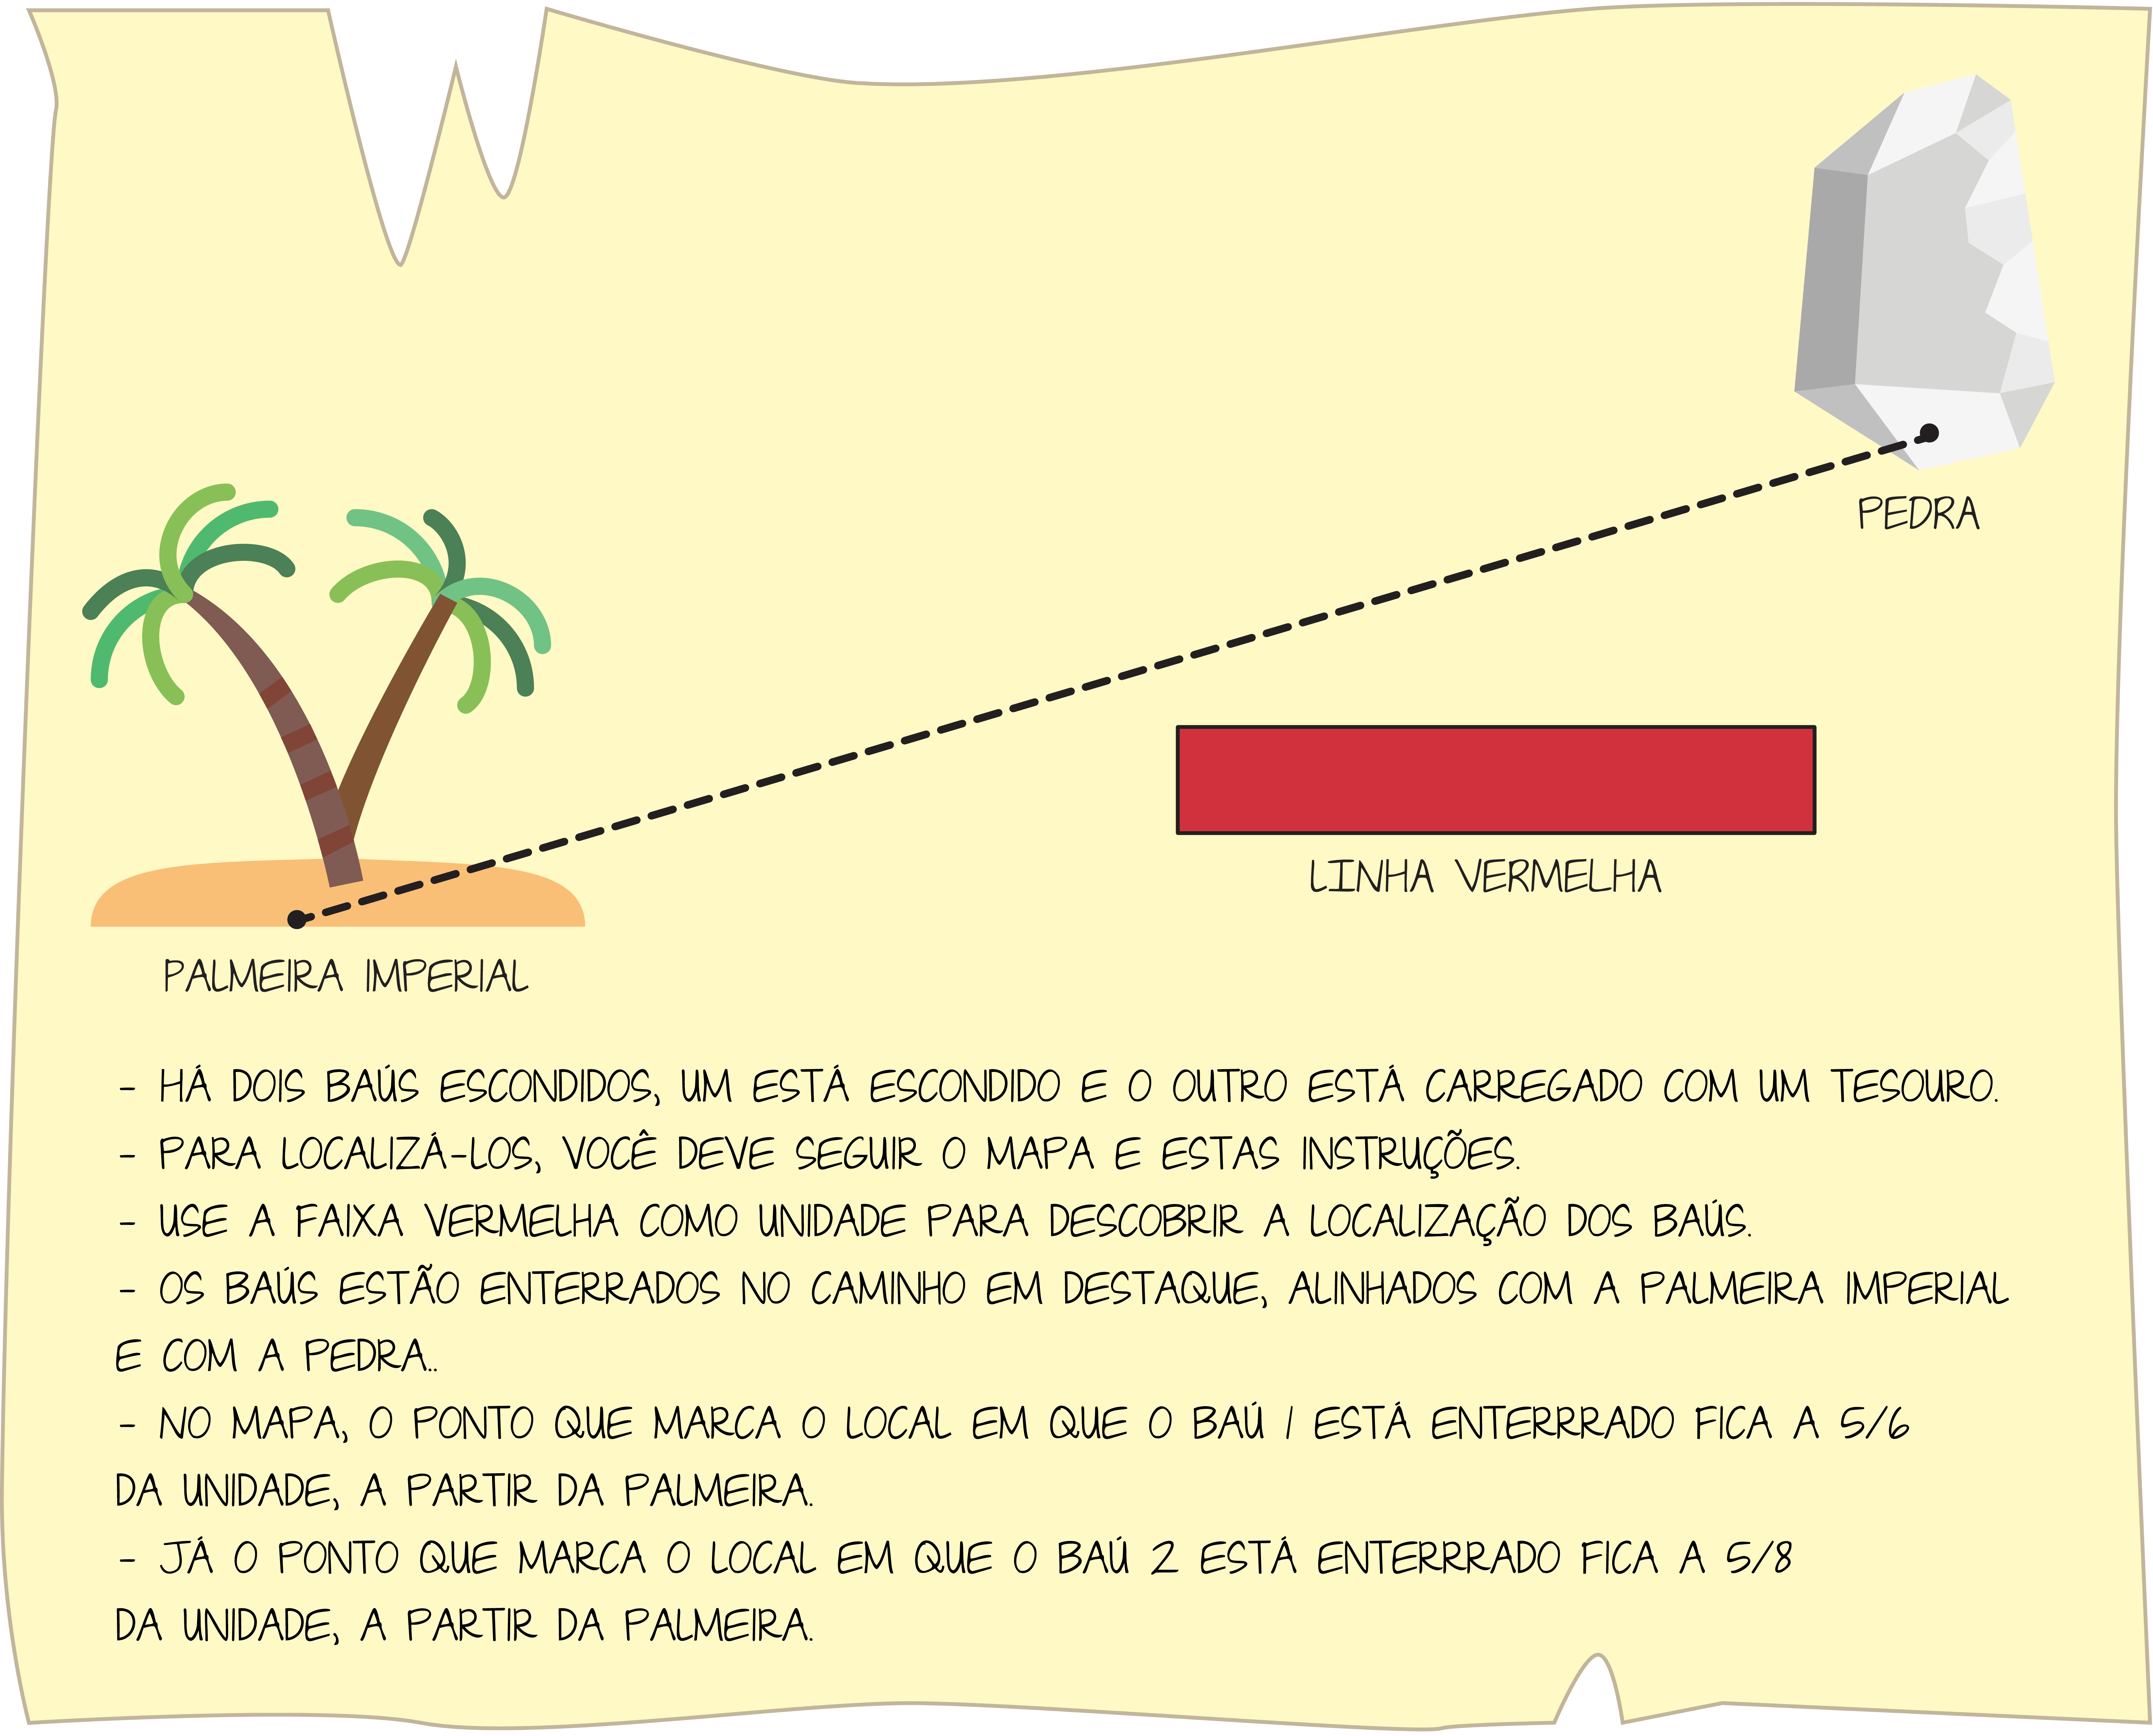
\includegraphics[width=\textwidth, keepaspectratio]{..//media//cap3/secoes/png/ativ7_fig01.png}  

\begin{enumerate}[a)]
 \item Marque, no mapa, as localizações dos baús 1 e 2.
 \item Qual o baú com o tesouro? Explique como chegou à sua conclusão. 
\end{enumerate}

\subsection{Atividade}

Três amigos foram a uma pizzaria e cada um pediu uma pizza média, de três sabores diferentes: João comeu $\frac{3}{4}$ da pizza de calabresa, Maria comeu  $\frac{2}{4}$ da pizza de presunto e Miguel comeu $\frac{3}{5}$ da pizza de milho. Sabendo que todas as pizzas eram do mesmo tamanho, pergunta-se:
\begin{enumerate} [\quad a)] %s
  \item     Quem comeu mais pizza, João ou Maria? Explique.
  \item     E no caso de João e Miguel, quem comeu mais pizza? Explique.
  \item     Dos três amigos, quem comeu mais pizza? Explique.
  \item     Marque na reta numérica a seguir as frações correspondentes às porções de pizza que cada amigo comeu, e confirme na reta numérica sua resposta em c.
\end{enumerate} %s

\begin{center}
 \begin{tikzpicture}[x=56.25mm,y=56.25mm]
\draw[->] (-0.2,0) -- (1.2,0) ; %edit here for the axis
\foreach \x in {0,1}{ \draw (\x,3pt) -- (\x,-3pt) node[below] {\x};}
\end{tikzpicture}  
\end{center}


\subsection{Atividade}

A imagem a seguir ilustra uma tartaruga percorrendo um caminho em linha reta, do ponto de partida ao de chegada. Observe a posição da tartaruga na imagem e avalie se as afirmações a seguir estão corretas ou não. Em cada item, explique a sua avaliação por escrito.
\begin{enumerate} [\quad a)] %s
  \item     A tartaruga percorreu mais do que a metade do percurso total.
  \item     A tartaruga percorreu mais do que     $\frac{3}{4}$     do percurso total.
  \item     A tartaruga percorreu mais do que     $\frac{3}{8}$     do percurso total.
  \item     A tartaruga percorreu menos do que     $\frac{3}{4}$     do percurso total.
  \item     A tartaruga percorreu menos do que     $\frac{2}{8}$     do percurso total.
  \item     A tartaruga percorreu menos do que     $\frac{2}{3}$     do percurso total.
  \item     A tartaruga percorreu     $\frac{3}{4}$     do percurso total.
  \item     A tartaruga percorreu pelo menos     $\frac{5}{8}$     do percurso total.
  \item     Para alcançar a chegada, a tartaruga precisa percorrer mais do que a metade do caminho.
  \item     Para alcançar a chegada, a tartaruga precisa percorrer menos do que     $\frac{2}{3}$     do caminho.
\end{enumerate} %s

  \noindent
\includegraphics[width=\textwidth, keepaspectratio]{..//media//cap3/secoes/png/ativ9_fig01.png}  

\subsection{Atividade}

Na figura, há várias retas paralelas igualmente espaçadas e outra reta, destacada em vermelho, não paralela às anteriores. Observe que as retas paralelas marcam na reta destacada em vermelho pontos também igualmente espaçados. Dois desses pontos correspondem ao 0 e ao 1. A reta vermelha torna-se uma reta numérica, como ilustra a figura. 

\begin{enumerate} [\quad a)] %s
  \item     Marque, usando os pontos destacados na reta numérica, a fração     $\frac{1}{2}$    . 
  \item     Associe frações a cada um dos pontos destacados na reta numérica. Explique a sua resposta.    \mbox{} \newline      
\begin{center}
 \begin{tikzpicture}[x=56.25mm,y=56.25mm]
 
\begin{scope}
\clip (-.2,-.2) rectangle (.85,.85); 
 
\begin{scope}[ rotate=45]
\foreach \x in {-1.1,-1,...,1.6}{
\draw[common] (\x,0) --+ (45:1); 
\draw[common] (\x,0) --+ (45:-1);}
 
\draw[attention] (-0.2,0) -- (1.2,0) ; %edit here for the axis
\foreach \x in {0,1}{ \draw (\x,3pt) -- (\x,-3pt) node[below] {\x};}
\foreach \x in {0.1,.2,...,.9}{ \draw (\x,3pt) -- (\x,-3pt);}
\end{scope}
\end{scope}
 
\end{tikzpicture}  
\end{center}

Como na figura anterior, há várias retas paralelas igualmente espaçadas e outra reta, destacada em azul, não paralela às anteriores. Observe que as retas paralelas marcam na reta destacada em azul pontos também igualmente espaçados. Dois desses pontos correspondem às frações $\frac{1}{2}$ e $\frac{3}{2}$, como ilustra a figura. 

  \item     Marque, usando os pontos destacados na reta numérica, os pontos correspondentes ao 0 e ao 1.
  \item     Marque, nesta mesma reta numérica, as frações     $\frac{3}{4}$     e     $\frac{5}{4}$    .
\begin{center}
  \begin{tikzpicture}[x=56.25mm,y=56.25mm]
 
\begin{scope}
\clip (-.2,-.2) rectangle (.85,.85); 
 
\begin{scope}[ rotate=45]
\foreach \x in {-1.1,-1,...,1.6}{
\draw[common] (\x,0) --+ (135:1); 
\draw[common] (\x,0) --+ (135:-1);}
 
\draw[blue] (-0.2,0) -- (1.2,0) ; %edit here for the axis
\foreach \x in {0,0.1,.2,...,.9}{ \draw (\x,3pt) -- (\x,-3pt);}
\fill[common] (.2,0) circle (3pt) node[below, black] {$\frac{1}{2}$};
\fill[common] (.6,0) circle (3pt) node[below, black] {$\frac{3}{2}$};
\end{scope}
\end{scope}
 
\end{tikzpicture}
\end{center}

\end{enumerate} %s

\section{ORGANIZANDO AS IDEIAS }


{\bf Frações na reta numérica}

Já é conhecido que os números naturais podem ser representados por pontos em uma reta. 
Para isso, é preciso começar escolhendo dois pontos que vão corresponder ao 0 e ao 1 e, a partir deles, são marcados os pontos que corresponderão aos demais números naturais.

\begin{center}
 \begin{tikzpicture}[x=18mm,y=18mm]
\draw[very thick, attention] (0,0) -- (1,0); 
\node[above] at (.5,0) {unidade};
\draw[->] (-0.5,0) -- (7.5,0) ; %edit here for the axis
\foreach \x in {0,1}{ \draw (\x,3pt) -- (\x,-3pt) node[below] {\x};}
\foreach \x in {0,1}{ \fill[common] (\x,0) circle (3pt);}
 
\end{tikzpicture}   
\end{center}
\vspace{.2cm}

\begin{center}
\begin{tikzpicture}[x=18mm,y=18mm]
 
\begin{scope}[shift={(0,.6)}]
\draw[very thick, attention] (0,0) -- (2,0);% segmento superior
\node[above] at (1,0) {2 unidades};
\foreach \x in {0,1,2}{ \draw (\x,3pt) -- (\x,-3pt);}% marcas verticais
\foreach \x in {0,2} \draw[very thick, ->] (\x,-.1) -- (\x,-.5); 
\end{scope}
 
\draw[->] (-0.5,0) -- (7.5,0) ; %reta anterior
\draw[very thick, attention] (0,0) -- (1,0); 
\foreach \x in {0,1,2}{ \draw (\x,3pt) -- (\x,-3pt) node[below] {\x};}
 
\foreach \x in {0,1,2}{ \fill[common] (\x,0) circle (3pt);}
 
\end{tikzpicture}   
 \end{center}
\vspace{.2cm}

\begin{center} 
\begin{tikzpicture}[x=18mm,y=18mm]
 
\begin{scope}[shift={(0,.6)}]
\draw[very thick, attention] (0,0) -- (7,0);% segmento superior
\node[above] at (3.5,0) {7 unidades};
\foreach \x in {0,1,...,7}{ \draw (\x,3pt) -- (\x,-3pt);}% marcas verticais
\foreach \x in {0,7} \draw[very thick, ->] (\x,-.1) -- (\x,-.5); 
\end{scope}
 
\draw[->] (-0.5,0) -- (7.5,0) ; %reta anterior
\draw[very thick, attention] (0,0) -- (1,0); 
\foreach \x in {0,1,7}{ \draw (\x,3pt) -- (\x,-3pt) node[below] {\x};}
 
\foreach \x in {0,1,7}{ \fill[common] (\x,0) circle (3pt);}
 
\end{tikzpicture}   
\end{center}

As frações também podem ser associadas a pontos na reta numérica. Para isso, é preciso identificar o segmento unitário, aquele cujos extremos são os pontos correspondentes ao 0 e ao 1. Esse segmento representa a unidade.
\begin{center}
\begin{tikzpicture}[x=18mm,y=18mm]
\draw[->] (-0.5,0) -- (7.5,0) ; %edit here for the axis
\foreach \x in {0,1}{ \draw (\x,3pt) -- (\x,-3pt) node[below] {\x};}
\draw[very thick, attention] (0,0) -- (1,0);
\foreach \x in {0,1}{ \fill[common] (\x,0) circle (3pt);}
\end{tikzpicture}   
\end{center}

Dividindo-se a unidade em partes iguais,  cada uma das partes identifica uma fração da unidade na reta numérica.
Por exemplo, a divisão da unidade em 3 partes iguais identifica terços. O ponto correspondente a $\frac{1}{3}$  é a extremidade do segmento que, a partir do 0, identifica o primeiro terço da unidade. 

\begin{center}
\begin{tikzpicture}[x=18mm,y=18mm]
 
\begin{scope}[shift={(0,.6)}]
\draw[very thick, attention] (0,0) -- (1/3,0);% segmento superior
\node[above] at (1/3,0) {$\frac{1}{3}$ da unidade};
\foreach \x in {0,1/3}{ \draw (\x,3pt) -- (\x,-3pt);}% marcas verticais
\foreach \x in {0,1/3} \draw[very thick, ->] (\x,-.1) -- (\x,-.5); 
\end{scope}
 
\draw[->] (-0.5,0) -- (3.5,0) ; %reta anterior
\draw[very thick, attention] (0,0) -- (1,0); 
\foreach \x in {0,1,...,3}{ \draw (\x,3pt) -- (\x,-3pt) node[below] {\x};}
 
\draw (2/3,3pt) -- (2/3,-3pt);
\node[below] at (1/3,0) {$\dfrac{1}{3}$};
\foreach \x in {0,1}{ \fill[common] (\x,0) circle (3pt);}
\fill[common] (1/3,0) circle (2pt);
\end{tikzpicture}
\end{center}


A partir dele, por justaposições desse segmento, são identificados na reta numérica os pontos correspondentes a $\frac{2}{3}$,$\frac{3}{3}$,$\frac{4}{3}$, e assim por diante. 



\begin{center}
\begin{tikzpicture}[x=18mm,y=18mm]
 
\begin{scope}[shift={(0,.6)}]
\draw[very thick, attention] (0,0) -- (2/3,0);% segmento superior
\node[above] at (1/3,0) {$\frac{2}{3}$ da unidade};
\foreach \x in {0,1/3, 2/3}{ \draw (\x,3pt) -- (\x,-3pt);}% marcas verticais
\foreach \x in {0,2/3} \draw[very thick, ->] (\x,-.1) -- (\x,-.5); 
\end{scope}
 
\draw[->] (-0.5,0) -- (3.5,0) ; %reta anterior
\draw[very thick, attention] (0,0) -- (1,0); 
\foreach \x in {0,1,...,3}{ \draw (\x,3pt) -- (\x,-3pt) node[below] {\x};}
 
\draw (2/3,3pt) -- (2/3,-3pt);
\node[below] at (1/3,0) {$\dfrac{1}{3}$};
\node[below] at (2/3,0) {$\dfrac{2}{3}$};
\foreach \x in {0,1}{ \fill[common] (\x,0) circle (3pt);}
\fill[common] (1/3,0) circle (2pt);
\fill[common] (2/3,0) circle (2pt);
\end{tikzpicture}   
\vspace{.2cm}

\begin{tikzpicture}[x=18mm,y=18mm]
\draw[->] (-0.5,0) -- (3.5,0) ; %reta anterior
\draw[very thick, attention] (0,0) -- (1,0); 
\foreach \x in {0,1,...,3}{ \draw (\x,3pt) -- (\x,-3pt);
\node[above] at (\x,3pt) {\x};}
 
\foreach \x in {0,3,...,9}{ \fill[common] (\x/3,0) circle (3pt);
\node[below] at (\x/3,0) {$\dfrac{\x}{3}$};}
 
\foreach \x in {1,2,4,5,7,8,10}{ \fill[common] (\x/3,0) circle (2pt);
\node[below] at (\x/3,0) {$\dfrac{\x}{3}$};}
 
\end{tikzpicture}   
\end{center}

A representação dos números na reta numérica ajuda a perceber que os pontos correspondentes a algumas frações  são os mesmos que os correspondentes a alguns números naturais. Por exemplo, $\frac{3}{3}$ é igual a 1. Portanto, $\frac{3}{3}$ de uma pizza é igual a 1 pizza e $\frac{3}{3}$ de uma barra de chocolate é igual a 1 barra de chocolate.

\begin{center}
\begin{tabular}{cc}
\noindent
\includegraphics[width=100pt, keepaspectratio]{..//media//cap3/secoes/png/orgideias_fig_a.png}  &
\noindent
\includegraphics[width=100pt, keepaspectratio]{..//media//cap3/secoes/png/orgideias_fig_b.png} \\
\begin{tikzpicture}[x=18mm,y=18mm]
 
\draw[->] (-0.5,0) -- (3.5,0) ; %reta anterior
\draw[very thick, attention] (0,0) -- (1,0); 
\foreach \x in {0,1,...,3}{ \draw (\x,3pt) -- (\x,-3pt);
\node[above] at (\x,3pt) {\x};}
 
\draw (1/3,3pt) -- (1/3,-3pt);
\draw (2/3,3pt) -- (2/3,-3pt);
\node[below] at (1/3,0) {$\dfrac{1}{3}$};
\node[below] at (2/3,0) {$\dfrac{2}{3}$};
%\foreach \x in {0,1/3,2/3,1}{ \fill[common] (\x,0) circle (3pt);}
 
\end{tikzpicture}   &
\begin{tikzpicture}[x=18mm,y=18mm]
 
\draw[->] (-0.5,0) -- (3.5,0) ; %reta anterior
\draw[very thick, attention] (0,0) -- (1,0); 
\foreach \x in {0,1,...,3}{ \draw (\x,3pt) -- (\x,-3pt);
\node[above] at (\x,3pt) {\x};}
 
\draw (1/3,3pt) -- (1/3,-3pt);
\draw (2/3,3pt) -- (2/3,-3pt);
% \node[below] at (1/3,0) {$\dfrac{1}{3}$};
% \node[below] at (2/3,0) {$\dfrac{2}{3}$};
\node[below] at (3/3,0) {$\dfrac{3}{3}$};
%\foreach \x in {0,1/3,2/3,1}{ \fill[common] (\x,0) circle (3pt);}
\end{tikzpicture}   
\end{tabular}
\end{center}

Já $\frac{6}{3}$ é igual a 2. Assim, $\frac{6}{3}$ de uma pizza é igual a 2 pizzas e $\frac{6}{3}$ de uma barra de chocolate é igual a 2 barras de chocolate.

\begin{center}
\begin{tabular}{cc}
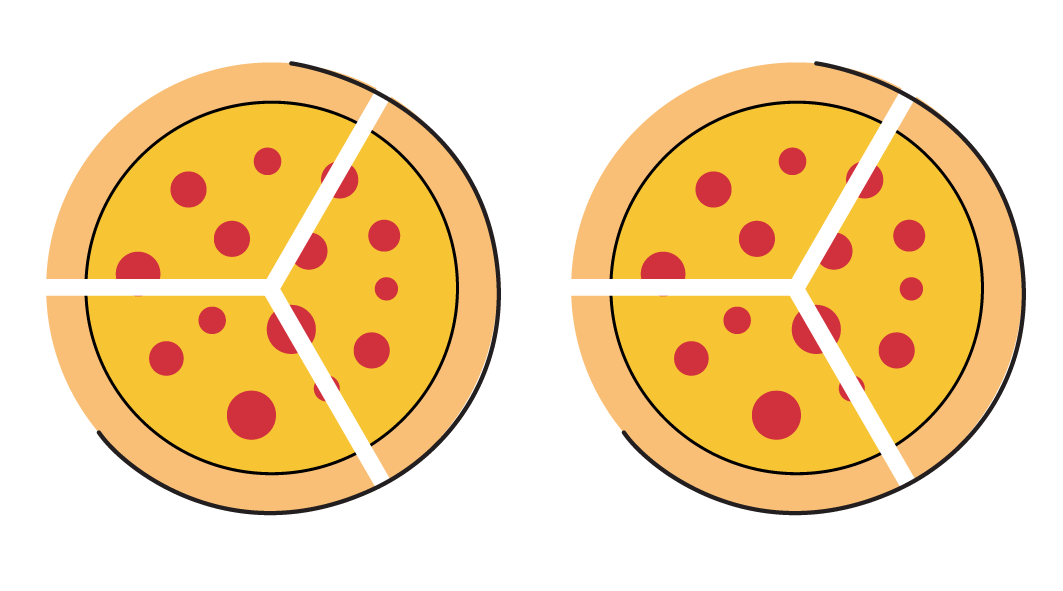
\includegraphics[width=200pt, keepaspectratio]{..//media//cap3/secoes/png/orgideias_fig_a_2.png} & 

\includegraphics[width=110pt, keepaspectratio]{..//media//cap3/secoes/png/orgideias_fig_b_2.png} \\
\begin{tikzpicture}[x=18mm,y=18mm]
 
\draw[->] (-0.5,0) -- (3.5,0) ; %reta anterior
\draw[very thick, attention] (0,0) -- (1,0); 
\foreach \x in {0,1,...,3}{ \draw (\x,3pt) -- (\x,-3pt);
\node[above] at (\x,3pt) {\x};}
 
\foreach \x in {1,...,5}{\draw (\x/3,3pt) -- (\x/3,-3pt);
\node[below] at (\x/3,0) {$\dfrac{\x}{3}$};}
 
\end{tikzpicture}     &
\begin{tikzpicture}[x=18mm,y=18mm]
 
\draw[->] (-0.5,0) -- (3.5,0) ; %reta anterior
\draw[very thick, attention] (0,0) -- (1,0); 
\foreach \x in {0,1,...,3}{ \draw (\x,3pt) -- (\x,-3pt);
\node[above] at (\x,3pt) {\x};}
 
\draw (1/3,3pt) -- (1/3,-3pt);
\draw (2/3,3pt) -- (2/3,-3pt);
\node[below] at (6/3,0) {$\dfrac{6}{3}$};
\end{tikzpicture}    
\end{tabular}
\end{center}




E $\frac{12}{3}$, é igual a que número natural? $\frac{12}{3}=$

Para identificar na reta numérica os pontos correspondentes às frações $\frac{1}{4}$, $\frac{2}{4}$, $\frac{3}{4}$, $\frac{4}{4}$,$\frac{5}{4}$, $\frac{6}{4}$, e assim por diante, o processo é o mesmo:

\begin{center}
 \begin{tikzpicture}[x=18mm,y=18mm]
\draw[->] (-0.5,0) -- (4.75,0) ; %reta anterior
\draw[very thick, attention] (0,0) -- (1,0); 
\foreach \x in {0,1,...,4}{ \draw (\x,3pt) -- (\x,-3pt);
\node[above] at (\x,3pt) {\x};}
 
\foreach \x in {0,1,...,18}{ \fill[common] (\x/4,0) circle (2pt);
\node[below] at (\x/4,0) {$\dfrac{\x}{4}$};}
 
\foreach \x in {0,4,...,16}{ \fill[common] (\x/4,0) circle (3pt);
\node[below] at (\x/4,0) {$\dfrac{\x}{4}$};}
\end{tikzpicture}   
\end{center}

Na reta numérica a seguir estão destacados alguns pontos e as frações correspondentes a eles. Observe e complete as frações em destaque indicando seus numeradores.

\begin{center}
 \begin{tikzpicture}[x=18mm,y=18mm]
\draw[->] (-0.5,0) -- (3.5,0) ; %reta anterior
\draw[very thick, attention] (0,0) -- (1,0); 
\foreach \x in {0,1,...,20}{ \draw (\x/6,3pt) -- (\x/6,-3pt);}
\foreach \x in {0,1,...,3}{ \draw (\x,3pt) -- (\x,-3pt) node[below] {\x};}
 
\foreach \x in {4,15,20}{ \fill[common] (\x/6,0) circle (3pt);
\node[below] at (\x/6,-9pt) {$\dfrac{}{6}$};}
 
\foreach \x in {2,9}{ \node[below] at (\x/6,-3pt) {$\dfrac{\x}{6}$};}
 
\end{tikzpicture}  
\end{center}

{\bf A ordem na reta numérica}

Na reta numérica, os números são organizados em ordem crescente, a partir do zero no sentido do 1. Assim, o que vale para o 0, o 1, o 2, o 3, etc. também valerá para as frações: 

\begin{center}
\begin{tikzpicture}[x=36mm,y=36mm]
 
\begin{scope}[shift={(0,150pt)}]
\draw[->] (-0.1,0) -- (3.5,0) ; %reta anterior
\draw[very thick, attention] (0,0) -- (1,0); 
\foreach \x in {0,1,...,3}{ \draw (\x,3pt) -- (\x,-3pt);
\foreach \x in {0,1,...,6}{ \draw (\x/2,3pt) -- (\x/2,-3pt);}
\node[above] at (\x,3pt) {\x};}
\foreach \x in {1,...,6} \node[below, light] at (\x/2 , 0 pt) {$\frac{\x}{2}$};
\end{scope}
 
\begin{scope}[shift={(0,100pt)}]
\draw[->] (-0.1,0) -- (3.5,0) ; %reta anterior
\draw[very thick, attention] (0,0) -- (1,0); 
\foreach \x in {0,1,...,3}{ \draw (\x,3pt) -- (\x,-3pt);
\foreach \x in {0,1,...,17}{ \draw (\x/5,2pt) -- (\x/5,-2pt);}
\node[above] at (\x,3pt) {\x};}
\foreach \x in {1,...,17} \node[below, attention] at (\x/5 , 0 pt) {$\frac{\x}{5}$};
\end{scope}
 
\begin{scope}[shift={(0,50pt)}]
\draw[->] (-0.1,0) -- (3.5,0) ; %reta anterior
\draw[very thick, attention] (0,0) -- (1,0); 
\foreach \x in {0,1,...,3}{ \draw (\x,3pt) -- (\x,-3pt);
\foreach \x in {0,1,...,34}{ \draw (\x/10,1pt) -- (\x/10,-1pt);}
\node[above] at (\x,3pt) {\x};}
\foreach \x in {0,...,34} \node[below, dark] at (\x/10,0) {$\frac{\x}{10}$};
\end{scope}
 
\draw[->] (-0.1,0) -- (3.5,0) ; %reta anterior
\draw[very thick, attention] (0,0) -- (1,0); 
\foreach \x in {0,1,...,3}{ \draw (\x,3pt) -- (\x,-3pt);
\node[above] at (\x,3pt) {\x};}
 
\foreach \x in {0,1,...,34}{ \draw (\x/10,1pt) -- (\x/10,-1pt);}
\foreach \x in {0,1,...,17}{ \draw (\x/5,2pt) -- (\x/5,-2pt);}
\foreach \x in {0,1,...,6}{ \draw (\x/2,3pt) -- (\x/2,-3pt);}
 
\foreach \x in {0,...,34} \node[below, dark] at (\x/10,0) {$\frac{\x}{10}$};
\foreach \x in {1,2,3,4,6,7,8,9,11,12,13,14,16,17} \node[above, attention] at (\x/5 , 3 pt) {$\frac{\x}{5}$};
\foreach \x in {1,3,5} \node[above, light] at (\x/2 , 3 pt) {\large $\frac{\x}{2}$};
 
\end{tikzpicture}   
\end{center}


Na reta numérica, quanto mais distante do 0 estiver o ponto correspondente ao número, maior será o número. 
\begin{center}
\begin{tikzpicture}[x=54mm,y=54mm]
\draw[->] (-0.5,0) -- (1.5,0) ; %reta anterior
\draw[very thick, attention] (0,0) -- (1,0); 
\foreach \x in {0,1}{ \draw (\x,3pt) -- (\x,-3pt);
\node[below] at (\x,0pt) {\x};}
 
% \node[below] at (1/3,0) {$\dfrac{1}{3}$};
% \node[below] at (2/3,0) {$\dfrac{2}{3}$};
%\node[below] at (6/3,0) {$\dfrac{6}{3}$};
\foreach \x in {3,5}{ \fill[common] (4/\x,0) circle (3pt);
\node[below] at (4/\x,0) {$\dfrac{4}{\x}$};}
 
\end{tikzpicture}
\end{center}

$\frac{4}{3}$ é maior do que $\frac{4}{5}$. Ou ainda, $\frac{4}{5}$ é menor do que $\frac{4}{3}$.


O símbolo é usado $<$ para dizer ``menor do que''.

Por exemplo, a frase ``oito é menor do que quinze'' pode ser expressa de modo mais resumido com ``$8<15$''. Já a expressão $\frac{1}{2}<\frac{3}{2}$ indica que ``um meio é menor do que três meios''.

Do mesmo modo, o símbolo $>$ é usado para significar ``maior do que'', portanto, também pode-se escrever $15>8$ para expressar ``quinze é maior do que oito'' ou $\frac{3}{2}>\frac{1}{2}$  para expressar ``três meios é maior do que um meio''
\begin{center}
  
\includegraphics[width=300pt, keepaspectratio]{..//media//cap3/secoes/png/orgideias_fig05.png}   
\end{center}
  
\section{MÃO NA MASSA }

\subsection{Atividade}

{\bf Jogo: varal dos números}

O varal de números está disposto na sala de aula, nele já estão posicionados os números $0$ (zero) e $1$ (um), como na figura. Nos cartões preparados para a atividade estão os números: \\
$0$, $1$, $2$, $3$, $\frac{1}{2}$, $\frac{2}{2}$, $\frac{3}{2}$, $\frac{4}{2}$, $\frac{5}{2}$, $\frac{6}{2}$,
$\frac{1}{3}$, $\frac{2}{3}$, $\frac{3}{3}$, $\frac{4}{3}$, $\frac{7}{3}$, $\frac{9}{3}$,
$\frac{1}{4}$, $\frac{2}{4}$, $\frac{3}{4}$, $\frac{4}{4}$, $\frac{5}{4}$, $\frac{6}{4}$, $\frac{8}{4}$, $\frac{10}{4}$, $\frac{11}{4}$, $\frac{12}{4}$,
$\frac{1}{5}$, $\frac{3}{5}$, $\frac{4}{5}$, $\frac{6}{5}$, $\frac{7}{5}$, $\frac{10}{5}$,
$\frac{1}{10}$.

\begin{center}

\includegraphics[width=300pt, keepaspectratio]{..//media//cap3/secoes/png/ativ11_fig01.png} 
\end{center}


O jogo consiste em fixar cartões numerados em varal, reproduzindo uma reta numérica. As regras serão apresentadas pelo seu professor ou professora. Discuta com seus colegas a posição correta de fixação de cada um dos cartões numerados no varal. 

Ao final do jogo, reproduza a forma como os cartões foram posicionados no varal na reta numérica a seguir. Aproveite as marcações já existentes.

\begin{center}
\begin{tikzpicture}[x=34mm,y=34mm]
\draw[->] (-0.1,0) -- (4,0) ; %reta anterior
\foreach \x in {0,.1,...,3.9}{ \draw (\x,3pt) -- (\x,-3pt);}
\end{tikzpicture}
\end{center}

\subsection{Atividade}

Na reta numérica já estão marcados o 0, o 1 e a fração $\frac{1}{2}$. Marque $\frac{3}{2}$, $\frac{3}{4}$, $\frac{5}{4}$, $\frac{8}{4}$, $\frac{10}{4}$, $\frac{1}{8}$, $\frac{7}{8}$, $\frac{10}{8}$ e 2.

\begin{center}
 \begin{tikzpicture}[x=5mm,y=5mm]
	\draw[->]  (-0.5,0) -- (26,0);
	\draw  (0,-3pt) -- (0,3pt);
	\draw  (1.25,-3pt) -- (1.25,3pt);
	\draw  (2.5,-3pt) -- (2.5,3pt);
	\draw  (3.75,-3pt) -- (3.75,3pt);
	\draw  (5,-3pt) -- (5,3pt);
	\draw  (6.25,-3pt) -- (6.25,3pt);
	\draw  (7.5,-3pt) -- (7.5,3pt);
	\draw  (8.75,-3pt) -- (8.75,3pt);
	\draw  (10,-3pt) -- (10,3pt);
	\draw  (11.25,-3pt) -- (11.25,3pt);
	\draw  (12.5,-3pt) -- (12.5,3pt);
	\draw  (13.75,-3pt) -- (13.75,3pt);
	\draw  (15,-3pt) -- (15,3pt);
	\draw  (16.25,-3pt) -- (16.25,3pt);
	\draw  (17.5,-3pt) -- (17.5,3pt);
	\draw  (18.75,-3pt) -- (18.75,3pt);
	\draw  (20,-3pt) -- (20,3pt);
	\draw  (21.25,-3pt) -- (21.25,3pt);
	\draw  (22.5,-3pt) -- (22.5,3pt);
	\draw  (23.75,-3pt) -- (23.75,3pt);
	\draw  (25,-3pt) -- (25,3pt);

	\node[below] at (0,0) {0};
	\node[below] at (5,0) {$\frac{1}{2}$};
	\node[below] at (10,0)  {1};

\end{tikzpicture}
\end{center}

\subsection{Atividade}


Associe, como no exemplo, cada uma das frações à sua representação na reta numérica.   

\noindent\begin{tabular}{m{.09\textwidth}m{.08\textwidth}m{.08\textwidth}m{.08\textwidth}m{.08\textwidth}m{.08\textwidth}m{0.08\textwidth}m{.08\textwidth}m{0.08\textwidth}}
(A) $\frac{1}{2}$ & (B) $\frac{1}{3}$ &  (C) $\frac{1}{4}$  & (D) $\frac{1}{5}$ & (E) $\frac{1}{6}$  & (F) $\frac{1}{7}$  & (G) $\frac{1}{8}$  & (H) $\frac{1}{9}$  & (I) $\frac{1}{10}$
\end{tabular}

\begin{center}
\begin{longtable}{m{.2\textwidth}m{.5\textwidth}}

\centering \begin{tikzpicture}
 \draw (0,0) -- (20,0);
\end{tikzpicture}
 & 
\parbox[t][1cm][c]{8cm}{
\begin{tikzpicture}[x=50mm,y=50mm]
\draw[->] (-0.3,0) -- (1.3,0) ; %reta anterior
\foreach \x in {0,.1,1}{ \draw (\x,3pt) -- (\x,-3pt);}
 \node[below] at (0,0) {0}; 
 \node[below] at (1,0) {1};
 \fill[common] (.1,0) circle (3pt);
\end{tikzpicture}}
\\
 
 \centering \begin{tikzpicture}
 \draw (0,0) -- (20,0);
 \node[above] at (10,0){(A)};
\end{tikzpicture}
 & 
\parbox[t][1cm][c]{8cm}{
\begin{tikzpicture}[x=50mm,y=50mm]
\draw[->] (-0.3,0) -- (1.3,0) ; %reta anterior
\foreach \x in {0,1}{ \draw (\x,3pt) -- (\x,-3pt);}
 \node[below] at (0,0) {0}; 
 \node[below] at (1,0) {1};
 \fill[common] (.5,0) circle (3pt);
\end{tikzpicture}
}\\
 
\centering \begin{tikzpicture}
 \draw (0,0) -- (20,0);
\end{tikzpicture}
  & 
\parbox[t][1cm][c]{8cm}{
\begin{tikzpicture}[x=50mm,y=50mm]
\draw[->] (-0.3,0) -- (1.3,0) ; %reta anterior
\foreach \x in {0,1}{ \draw (\x,3pt) -- (\x,-3pt);}
 \node[below] at (0,0) {0}; 
 \node[below] at (1,0) {1};
 \fill[common] (1/3,0) circle (3pt);
\end{tikzpicture}
}\\
  
\centering \begin{tikzpicture}
 \draw (0,0) -- (20,0);
\end{tikzpicture}
 & 
\parbox[t][1cm][c]{8cm}{
\begin{tikzpicture}[x=50mm,y=50mm]
\draw[->] (-0.3,0) -- (1.3,0) ; %reta anterior
\foreach \x in {0,1}{ \draw (\x,3pt) -- (\x,-3pt);}
 \node[below] at (0,0) {0}; 
 \node[below] at (1,0) {1};
 \fill[common] (1/9,0) circle (3pt);
\end{tikzpicture}
}\\
 
\centering \begin{tikzpicture}
 \draw (0,0) -- (20,0);
\end{tikzpicture}
 & 
\parbox[t][1cm][c]{8cm}{
\begin{tikzpicture}[x=50mm,y=50mm]
\draw[->] (-0.3,0) -- (1.3,0) ; %reta anterior
\foreach \x in {0,1}{ \draw (\x,3pt) -- (\x,-3pt);}
 \node[below] at (0,0) {0}; 
 \node[below] at (1,0) {1};
 \fill[common] (1/7,0) circle (3pt);
\end{tikzpicture}
}\\
 
\centering \begin{tikzpicture}
 \draw (0,0) -- (20,0);
\end{tikzpicture}
 & 
\parbox[t][1cm][c]{8cm}{
\begin{tikzpicture}[x=50mm,y=50mm]
\draw[->] (-0.3,0) -- (1.3,0) ; %reta anterior
\foreach \x in {0,1}{ \draw (\x,3pt) -- (\x,-3pt);}
 \node[below] at (0,0) {0}; 
 \node[below] at (1,0) {1};
 \fill[common] (.25,0) circle (3pt);
\end{tikzpicture}
}\\
 
\centering \begin{tikzpicture}
 \draw (0,0) -- (20,0);
\end{tikzpicture}
 & 
\parbox[t][1cm][c]{8cm}{
\begin{tikzpicture}[x=50mm,y=50mm]
\draw[->] (-0.3,0) -- (1.3,0) ; %reta anterior
\foreach \x in {0,1}{ \draw (\x,3pt) -- (\x,-3pt);}
 \node[below] at (0,0) {0}; 
 \node[below] at (1,0) {1};
 \fill[common] (1/6,0) circle (3pt);
\end{tikzpicture}
}\\
 
\centering \begin{tikzpicture}
 \draw (0,0) -- (20,0);
\end{tikzpicture}
& 
\parbox[t][1cm][c]{8cm}{
\begin{tikzpicture}[x=50mm,y=50mm]
\draw[->] (-0.3,0) -- (1.3,0) ; %reta anterior
\foreach \x in {0,1}{ \draw (\x,3pt) -- (\x,-3pt);}
 \node[below] at (0,0) {0}; 
 \node[below] at (1,0) {1};
 \fill[common] (1/5,0) circle (3pt);
\end{tikzpicture}
}\\
 
\centering \begin{tikzpicture}
 \draw (0,0) -- (20,0);
\end{tikzpicture}
& 
\parbox[t][1cm][c]{8cm}{
\begin{tikzpicture}[x=50mm,y=50mm]
\draw[->] (-0.3,0) -- (1.3,0) ; %reta anterior
\foreach \x in {0,1}{ \draw (\x,3pt) -- (\x,-3pt);}
 \node[below] at (0,0) {0}; 
 \node[below] at (1,0) {1};
 \fill[common] (1/8,0) circle (3pt);
\end{tikzpicture}
}\\
 
\end{longtable}
\end{center}

\subsection{Atividade}

Observando a atividade anterior (Atividade 13), complete as sentenças a seguir com os sinais $>$ (maior) ou $<$ (menor) de modo a torná-las verdadeiras.
\begin{center}
\begin{tabular}{ccccccccc}
 a)  &   $\dfrac{1}{2}$    & \parbox[t][.6cm]{2cm}{ }\quad\quad\quad      &  $\dfrac{1}{5}$ & \quad\quad\quad\quad\quad\quad\quad   &e)  &  $\dfrac{1}{35}$   & \quad\quad\quad      &  $\dfrac{1}{43}$\\
 b)  &  $\dfrac{1}{4}$    & \parbox[t][.6cm]{2cm}{ }      &  $\dfrac{1}{3}$   & & f)  &  $\dfrac{1}{99}$   &       &  $\dfrac{1}{100}$  \\
 c)  &  $\dfrac{1}{10}$   &  \parbox[t][.6cm]{2cm}{ }     &  $\dfrac{1}{20}$  & & g)  &  $\dfrac{1}{5}$    &       &  $\dfrac{1}{50}$  \\
 d)  &  $\dfrac{1}{12}$   & \parbox[t][.6cm]{2cm}{ }      &  $\dfrac{1}{2}$   & & h)  &  $\dfrac{1}{100}$  &       &  $\dfrac{1}{10}$  \\ 
 \end{tabular}
 \end{center}


\subsection{Atividade}

Na reta numérica a seguir estão destacados os pontos correspondentes ao 0, ao 1 e a $\frac{1}{2}$. Os demais pontos correspondem às frações apresentadas a seguir. Associe cada fração ao ponto correspondente.  

\begin{center}
\begin{tikzpicture}[x=.3cm,y=.3cm,]
	\draw[->] (-2,0) -- (47,0);
		
	\fill[common] (0,0) circle (3 pt);		%0
	\fill[common] (10,0) circle (3 pt);
	\fill[common] (15,0) circle (3 pt);
	\fill[common] (20,0) circle (3 pt);
	\fill[common] (25,0) circle (3 pt);
	\fill[common] (30,0) circle (3 pt);
	\fill[common] (32,0) circle (3 pt);
	\fill[common] (36,0) circle (3 pt);
	\fill[common] (40,0) circle (3 pt);
	\fill[common] (44,0) circle (3 pt);
	\fill[common] (45,0) circle (3 pt);

		\node[below]  at (0,-1) {0};			%0
		\node[below]  at (20,-1) {$\frac{1}{2}$};	%1/2
		\node[below]  at (40,-1) {1};			%1

	 	     \tikzstyle{gray_block} = [draw,outer sep=3,inner sep=3,minimum size=1,line width=1, very thick, draw=black!55, top color=white,bottom color=black!20]
	\node [gray_block] at (10.5,5) {$\frac{1}{4}$};   
  	\node [gray_block] at (14.5,5) {$\frac{3}{4}$};
	\node [gray_block] at (18.5,5) {$\frac{4}{5}$};
	\node [gray_block] at (22.5,5) {$\frac{3}{8}$};
	\node [gray_block] at (26.5,5) {$\frac{5}{8}$};
	\node [gray_block] at (30.5,5) {$\frac{9}{8}$};
	\node [gray_block] at (35,5) {$\frac{9}{10}$};
	\node [gray_block] at (40,5) {$\frac{11}{10}$};
\end{tikzpicture}
\end{center}

\subsection{Atividade}


Complete as sentenças a seguir com os sinais $>$ (maior), $<$ (menor) ou $=$ (igual) de modo a torná-las verdadeiras. 

\begin{center}
\begin{tabular}{lccccccccccccc}
 a)  &  $\dfrac{3}{6}$     &   &  $\dfrac{5}{6}$   & \parbox[t][.6cm]{2cm}{ } \quad \quad\quad  & f)  &  $\dfrac{1}{2}$     &   &  $\dfrac{1}{3}$    & \quad \quad\quad  & m)  &  $\dfrac{3}{2}$     &   &  $\dfrac{2}{5}$    \\
 b)  &  $\dfrac{5}{9}$     &   &  $\dfrac{4}{9}$   & \parbox[t][.6cm]{2cm}{ }    & g)  &  $\dfrac{1}{7}$     &   &  $\dfrac{1}{6}$    &   & n)  &  $\dfrac{3}{4}$     &   &  $\dfrac{6}{5}$    \\
 c)  &  $\dfrac{7}{10}$    &   &  $\dfrac{9}{10}$   & \parbox[t][.6cm]{2cm}{ }   & h)  &  $\dfrac{2}{5}$     &   &  $\dfrac{2}{7}$    &   & o)  &  $\dfrac{7}{8}$     &   &  $\dfrac{10}{9}$   \\
 d)  &  $\dfrac{3}{12}$    &   &  $\dfrac{9}{12}$   & \parbox[t][.6cm]{2cm}{ }   & i)  &  $\dfrac{4}{5}$     &   &  $\dfrac{4}{3}$    &   & p)  &  $\dfrac{6}{5}$     &   &  $\dfrac{12}{9}$   \\
 e)  &  $\dfrac{39}{100}$  &   &  $\dfrac{25}{100}$ & \parbox[t][.6cm]{2cm}{ }   & j)  &  $\dfrac{12}{15}$   &   &  $\dfrac{12}{7}$   &   & q)  &  $\dfrac{4}{5}$     &   &  $\dfrac{5}{4}$    \\
     &&                     &    &                  \parbox[t][.6cm]{2cm}{ }    &  l)  &  $\dfrac{22}{80}$   &   &  $\dfrac{22}{90}$  &   & r)  &  $\dfrac{35}{40}$   &   &  $\dfrac{30}{25}$  \\
     &&                      &    &                    &      &  \parbox[t][.6cm]{2cm}{ }                    &   &                   &   &  s)  &  $\dfrac{99}{100}$  &   &  $\dfrac{3}{2}$    \\
\end{tabular} 
 \end{center}
 
\section{QUEBRANDO A CUCA }


\subsection{Atividade}

Você recebeu uma folha com retângulos que têm o mesmo tamanho mas que são coloridos de maneira diferente. Em cada um deles há marcações que representam uma equipartição.  

\begin{enumerate}[a)]
\item Complete os retângulos, ecrevendo em cada um deles a fração representada por cada parte da equipartição, como no exemplo
\begin{center}
\begin{tikzpicture}[scale=.5]
\draw[fill=gray] (0,0) rectangle (60,12);
    \end{tikzpicture}

\begin{tikzpicture}[scale=.5]
\draw[fill=light] (0,0) rectangle (60,12);
\draw (30,0) -- (30,12);
\node at (15,6) {{\small $\frac{1}{2}$}};
\node at (45,6) {{\small $\frac{1}{2}$}};
\end{tikzpicture}
    
   \begin{tikzpicture}[scale=.5]
\draw[fill=pink] (0,0) rectangle (60,12);
\foreach \x in {1,2} \draw (\x*60/3,0) -- (\x*60/3,12);
    \end{tikzpicture}        
    
      \begin{tikzpicture}[scale=.5]
\draw[fill=special] (0,0) rectangle (60,12);
\foreach \x in {1,2,3} \draw (\x*60/4,0) -- (\x*60/4,12);
    \end{tikzpicture}        
    
   \begin{tikzpicture}[scale=.5]
\draw[fill=attention] (0,0) rectangle (60,12);
\foreach \x in {1,...,4} \draw (\x*60/5,0) -- (\x*60/5,12);
    \end{tikzpicture}        
    
   \begin{tikzpicture}[scale=.5]
\draw[fill=common] (0,0) rectangle (60,12);
\foreach \x in {1,...,5} \draw (\x*60/6,0) -- (\x*60/6,12);
    \end{tikzpicture}        
    
    \begin{tikzpicture}[scale=.5]
\draw[fill=CornflowerBlue] (0,0) rectangle (60,12);
\foreach \x in {1,...,6} \draw (\x*60/7,0) -- (\x*60/7,12);
    \end{tikzpicture}        
    
   \begin{tikzpicture}[scale=.5]
\draw[fill=dark] (0,0) rectangle (60,12);
\foreach \x in {1,...,7} \draw (\x*60/8,0) -- (\x*60/8,12);
    \end{tikzpicture}        
    
   \begin{tikzpicture}[scale=.5]
\draw[fill=Fuchsia] (0,0) rectangle (60,12);'
\foreach \x in {1,...,8} \draw (\x*60/9,0) -- (\x*60/9,12);
    \end{tikzpicture}        
    
 \begin{tikzpicture}[scale=.5]   
 \draw[fill=NavyBlue] (0,0) rectangle (60,12);
 \foreach \x in {1,...,9} \draw (\x*60/10,0) -- (\x*60/10,12);
     \end{tikzpicture}        
    
\begin{tikzpicture}[scale=.5]   
    \draw[fill=BlueViolet] (0,0) rectangle (60,12);
\foreach \x in {1,...,15} \draw (\x*60/16,0) -- (\x*60/16,12);
    \end{tikzpicture}        
 \end{center}
\item  Recorte os retângulos coloridos da folha que você recebeu e use-os para representar na reta numérica os seguintes números: 

$0$, $1$, $\frac{1}{2}$, $\frac{1}{3}$, $\frac{1}{4}$, $\frac{3}{4}$, $\frac{3}{5}$, $\frac{5}{6}$, $\frac{7}{6}$, $\frac{6}{7}$,  $\frac{10}{7}$,  $\frac{12}{7}$,  $\frac{10}{8}$,  $\frac{12}{8}$, $\frac{10}{9}$, $\frac{12}{9}$, $\frac{10}{10}$, $\frac{20}{16}$

\begin{center}
 \begin{tikzpicture}[scale=.5]
\draw[->] (-10,0) -- (150,0);
\foreach \x in {0,60} \draw (\x,-6pt) -- (\x,6 pt);
\node at (0,-20pt) {0};
\node at (60,-20pt) {1};
\end{tikzpicture}
\end{center}


\end{enumerate}


\subsection{Atividade}


Na reta numérica a seguir:
\begin{enumerate} [\quad a)] %s
  \item     Marque     $\frac{1}{2}$    . Justifique sua resposta.
  \item     Marque     $\frac{1}{4}$    ,     $\frac{3}{4}$     e     $\frac{5}{4}$    . Explique como raciocinou para fazer essas marcações. 
  
\begin{center}
\begin{tikzpicture}[x=15mm,y=15mm]
\draw[->] (-0.5,0) -- (5.5,0) ; %reta anterior
\foreach \x in {0,2}{ \draw (\x,3pt) -- (\x,-3pt);}
\node[below] at (0,0) {0};
\node[below] at (2,0) {2};
\end{tikzpicture}
\end{center}

Observando a reta numérica com as marcações feitas, compare: 

  \item $\frac{1}{4}$     é maior ou menor do que     $\frac{1}{2}$    ? 
  \item $\frac{3}{4}$ é maior ou menor do que $\frac{1}{2}$    ?
  \item $\frac{5}{4}$  é menor do que 1?
  \item Escreva as frações marcadas na reta em ordem crescente, completando os espaços a seguir:

$$0 < \frac{\square}{\square} < \frac{\square}{\square}< \frac{\square}{\square} < 1 < \frac{\square}{\square}$$

Volte à reta e marque outras três frações que atendam às seguintes condições: 
  \item A primeira deve ser maior do que $3$ e menor do que $4$.
 \item A segunda deve ser maior do que $\frac{7}{2}$.
 \item A terceira deve ser maior do que $\frac{17}{4}$ e menor do que $5$

\end{enumerate} %s



